\section*{1. Measuring Dependence: Covariance Structures}

When working with multivariate random vectors, characterizing how variables move in tandem is essential. The primary metric for tracking linear co-movement between two scalar random variables $X$ and $Y$ is \textbf{covariance}:
\begin{equation}
\text{Cov}[X, Y] \triangleq \mathbb{E}\left[(X - \mathbb{E}[X])(Y - \mathbb{E}[Y])\right] = \mathbb{E}[XY] - \mathbb{E}[X]\mathbb{E}[Y] \tag{1}
\end{equation}

\paragraph{The Multivariate Covariance Matrix}
For a $D$-dimensional random vector $\mathbf{x} = [X_1, X_2, \dots, X_D]^T \in \mathbb{R}^D$, we scale this concept into a symmetric, positive semi-definite matrix $\boldsymbol{\Sigma} \in \mathbb{R}^{D \times D}$. This matrix captures the dispersion of the entire vector about its multivariate mean vector $\boldsymbol{\mu} = \mathbb{E}[\mathbf{x}]$:
\begin{equation}
\boldsymbol{\Sigma} \triangleq \text{Cov}[\mathbf{x}] \triangleq \mathbb{E}\left[ (\mathbf{x} - \mathbb{E}[\mathbf{x}])(\mathbf{x} - \mathbb{E}[\mathbf{x}])^T \right] \tag{2}
\end{equation}

Evaluating the outer product inside the expectation expands into an explicit grid of variance and pairwise covariance elements:
\begin{equation}
\boldsymbol{\Sigma} = 
\begin{bmatrix}
\mathbb{V}[X_1] & \text{Cov}[X_1, X_2] & \cdots & \text{Cov}[X_1, X_D] \\
\text{Cov}[X_2, X_1] & \mathbb{V}[X_2] & \cdots & \text{Cov}[X_2, X_D] \\
\vdots & \vdots & \ddots & \vdots \\
\text{Cov}[X_D, X_1] & \text{Cov}[X_D, X_2] & \cdots & \mathbb{V}[X_D]
\end{bmatrix} \tag{3}
\end{equation}

\paragraph{Rigorous Proof: The Raw Second Moment Decomposition}
A critical identity in multivariate statistics relates the covariance matrix to the expected raw outer product $\mathbb{E}[\mathbf{x}\mathbf{x}^T]$. Let's derive this relationship from first principles:
\begin{align*}
\boldsymbol{\Sigma} &= \mathbb{E}\left[ (\mathbf{x} - \boldsymbol{\mu})(\mathbf{x} - \boldsymbol{\mu})^T \right] \\
&= \mathbb{E}\left[ \mathbf{x}\mathbf{x}^T - \mathbf{x}\boldsymbol{\mu}^T - \boldsymbol{\mu}\mathbf{x}^T + \boldsymbol{\mu}\boldsymbol{\mu}^T \right]
\end{align*}
Because expectation is a linear operator, and $\boldsymbol{\mu}$ is a deterministic vector constant, we distribute the expectation across each individual term:
\begin{align*}
\boldsymbol{\Sigma} &= \mathbb{E}[\mathbf{x}\mathbf{x}^T] - \mathbb{E}[\mathbf{x}]\boldsymbol{\mu}^T - \boldsymbol{\mu}\mathbb{E}[\mathbf{x}]^T + \boldsymbol{\mu}\boldsymbol{\mu}^T \\
&= \mathbb{E}[\mathbf{x}\mathbf{x}^T] - \boldsymbol{\mu}\boldsymbol{\mu}^T - \boldsymbol{\mu}\boldsymbol{\mu}^T + \boldsymbol{\mu}\boldsymbol{\mu}^T \\
&= \mathbb{E}[\mathbf{x}\mathbf{x}^T] - \boldsymbol{\mu}\boldsymbol{\mu}^T
\end{align*}
Rearranging terms yields the foundational identity:
\begin{equation}
\mathbb{E}[\mathbf{x}\mathbf{x}^T] = \boldsymbol{\Sigma} + \boldsymbol{\mu}\boldsymbol{\mu}^T \tag{4}
\end{equation}

\paragraph{Cross-Covariance Vectors}
When comparing two entirely distinct random vectors $\mathbf{x} \in \mathbb{R}^{D_1}$ and $\mathbf{y} \in \mathbb{R}^{D_2}$, their relationship is mapped via a non-square matrix known as the \textbf{cross-covariance matrix}:
\begin{equation}
\text{Cov}[\mathbf{x}, \mathbf{y}] \triangleq \mathbb{E}\left[ (\mathbf{x} - \mathbb{E}[\mathbf{x}])(\mathbf{y} - \mathbb{E}[\mathbf{y}])^T \right] \in \mathbb{R}^{D_1 \times D_2} \tag{5}
\end{equation}

\section*{2. Normalized Linear Relationships: Correlation Mechanics}

Because the raw scale of covariance depends on the arbitrary measurement units of the underlying variables, it can range from $-\infty$ to $+\infty$. To create a scale-invariant metric, we divide the covariance by the product of the individual standard deviations, yielding the \textbf{Pearson correlation coefficient}:
\begin{equation}
\rho \triangleq \text{corr}[X, Y] \triangleq \frac{\text{Cov}[X, Y]}{\sqrt{\mathbb{V}[X]\mathbb{V}[Y]}} \tag{6}
\end{equation}
By application of the Cauchy-Schwarz Inequality, this normalized value is bounded strictly within a standardized domain: $-1 \le \rho \le 1$.

\paragraph{Geometric and Algebraic Scaling of the Correlation Matrix}
For a multidimensional vector $\mathbf{x}$, the system-wide dependencies can be gathered into a \textbf{correlation matrix}, where every diagonal entry is identically $1$. This matrix can be expressed compactly via matrix algebra by sandwiching the auto-covariance matrix $\boldsymbol{\Sigma}$ between two copies of the inverse square root of the diagonalized variance matrix:
\begin{equation}
\text{corr}(\mathbf{x}) = \left(\text{diag}(\boldsymbol{\Sigma})\right)^{-\frac{1}{2}} \boldsymbol{\Sigma} \left(\text{diag}(\boldsymbol{\Sigma})\right)^{-\frac{1}{2}} \tag{7}
\end{equation}

\paragraph{Intuitive Numerical Walkthrough of Matrix Scaling}
Let's see how Equation (7) functions in practice with a concrete $2\times2$ covariance matrix system:
\begin{equation*}
\boldsymbol{\Sigma} = \begin{bmatrix} 4 & 3 \\ 3 & 9 \end{bmatrix}
\end{equation*}
Here, the marginal variance of $X_1$ is $\sigma_1^2 = 4$ and the variance of $X_2$ is $\sigma_2^2 = 9$.
\begin{enumerate}
    \item Isolate the diagonal elements: $\text{diag}(\boldsymbol{\Sigma}) = \begin{bmatrix} 4 & 0 \\ 0 & 9 \end{bmatrix}$.
    \item Compute the inverse square root of this diagonal configuration:
    \begin{equation*}
    \left(\text{diag}(\boldsymbol{\Sigma})\right)^{-\frac{1}{2}} = \begin{bmatrix} \frac{1}{\sqrt{4}} & 0 \\ 0 & \frac{1}{\sqrt{9}} \end{bmatrix} = \begin{bmatrix} 0.5 & 0 \\ 0 & \frac{1}{3} \end{bmatrix}
    \end{equation*}
    \item Apply the sandwich multiplication to evaluate Equation (7):
    \begin{align*}
    \text{corr}(\mathbf{x}) &= \begin{bmatrix} 0.5 & 0 \\ 0 & \frac{1}{3} \end{bmatrix} \begin{bmatrix} 4 & 3 \\ 3 & 9 \end{bmatrix} \begin{bmatrix} 0.5 & 0 \\ 0 & \frac{1}{3} \end{bmatrix} \\
    &= \begin{bmatrix} 2 & 1.5 \\ 1 & 3 \end{bmatrix} \begin{bmatrix} 0.5 & 0 \\ 0 & \frac{1}{3} \end{bmatrix} = \begin{bmatrix} 1 & 0.5 \\ 0.5 & 1 \end{bmatrix}
    \end{align*}
\end{enumerate}
This demonstrates how the sandwich operation normalizes the off-diagonal covariance entry ($\Sigma_{12} = 3$) into a scale-free correlation coefficient ($\rho = 0.5$).

\section*{3. Fundamental Pitfalls of Linear Dependence Metrics}

\paragraph{Pitfall 1: Uncorrelated Does Not Imply Independent}
If two random variables are independent, their joint density factorizes ($p(X,Y) = p(X)p(Y)$), making their covariance and correlation identically zero. \textbf{The converse is fundamentally false}: an auto-covariance of zero does not mean variables are independent. It simply indicates an absence of a \textit{linear} relationship.

\begin{tcolorbox}[colback=red!5!white, colframe=red!60!black, title=Analytical Counterexample Proof]
Let $X$ be distributed uniformly over a symmetric interval centered at zero: $X \sim \text{Unif}(-1, 1)$. Let $Y$ be defined deterministically by a non-linear quadratic mapping: $Y = X^2$. 

Clearly, $Y$ and $X$ are completely dependent. Let's calculate their covariance using Equation (1):
\begin{equation*}
\text{Cov}[X, Y] = \mathbb{E}[XY] - \mathbb{E}[X]\mathbb{E}[Y]
\end{equation*}
\begin{itemize}
    \item The mean of our uniform input is zero: $\mathbb{E}[X] = 0 \implies \mathbb{E}[X]\mathbb{E}[Y] = 0$.
    \item The first expectation term becomes: $\mathbb{E}[XY] = \mathbb{E}[X \cdot X^2] = \mathbb{E}[X^3]$.
\end{itemize}
By evaluating the expectation integral for an odd power across a symmetric domain:
\begin{equation*}
\mathbb{E}[X^3] = \int_{-1}^{1} x^3 \cdot \left(\frac{1}{2}\right) dx = \left[ \frac{x^4}{8} \right]_{-1}^{1} = \frac{1}{8} - \frac{1}{8} = 0
\end{equation*}
Consequently, \text{Cov}[X, Y] = 0 and \text{corr}[X, Y] = 0. This proves that a system can possess a flawless, deterministic functional dependency while maintaining a correlation score of zero.
\end{tcolorbox}

\paragraph{Pitfall 2: Correlation Does Not Imply Causation}
A high correlation coefficient indicates that two variables change together linearly, but it says nothing about the mechanism driving that change. Observed co-movements often stem from a hidden common cause (\textbf{confounding variable}). For example, ice cream sales and violent crime rates are strongly positively correlated, not because one causes the other, but because hot summer weather independently increases both metrics.

\paragraph{Pitfall 3: Simpson's Paradox}
When analyzing data, a correlation observed within an aggregated population can completely reverse its sign when the population is split into its constituent sub-groups. 

As seen in the Iris dataset, assessing the entire population might suggest a negative correlation between Sepal Length and Sepal Width ($\rho = -0.12$). However, conditioning the analysis on individual species reveals strong positive correlations within each isolated group (e.g., Setosa: $\rho = 0.74$). This underscores why predictive correlations must not be mistaken for structural causal models.

\section*{4. The Multivariate Gaussian Distribution: Definition and Geometry}

The most widely utilized joint probability distribution for continuous random variables is the \textbf{multivariate Gaussian} (or multivariate normal, MVN) distribution. Its ubiquity stems from its analytic tractability under linear transformations and its status as the limiting distribution under the Central Limit Theorem.

For a $D$-dimensional continuous random vector $\mathbf{y} \in \mathbb{R}^D$, the multivariate Gaussian probability density function (pdf) is defined as:
\begin{equation}
\mathcal{N}(\mathbf{y} \mid \boldsymbol{\mu}, \boldsymbol{\Sigma}) \triangleq \frac{1}{(2\pi)^{D/2}|\boldsymbol{\Sigma}|^{1/2}} \exp \left[ -\frac{1}{2}(\mathbf{y} - \boldsymbol{\mu})^T \boldsymbol{\Sigma}^{-1}(\mathbf{y} - \boldsymbol{\mu}) \right] \tag{8}
\end{equation}
where $\boldsymbol{\mu} = \mathbb{E}[\mathbf{y}] \in \mathbb{R}^D$ represents the mean vector, and $\boldsymbol{\Sigma} = \text{Cov}[\mathbf{y}] \in \mathbb{R}^{D \times D}$ is the symmetric, positive-definite covariance matrix. 

The scaling factor $Z = (2\pi)^{D/2}|\boldsymbol{\Sigma}|^{1/2}$ represents the \textbf{normalization constant}, ensuring that the density integrates to unity across the entire vector space:
\begin{equation*}
\int_{\mathbb{R}^D} \mathcal{N}(\mathbf{y} \mid \boldsymbol{\mu}, \boldsymbol{\Sigma}) \, d\mathbf{y} = 1
\end{equation*}
The term inside the exponential function, $\Delta^2 = (\mathbf{y} - \boldsymbol{\mu})^T \boldsymbol{\Sigma}^{-1}(\mathbf{y} - \boldsymbol{\mu})$, is known as the \textbf{Mahalanobis distance} between the random vector $\mathbf{y}$ and its mean $\boldsymbol{\mu}$. It accounts for both the variance of individual dimensions and the linear dependencies between them.

\section*{5. The Bivariate Case: Explicit Deconstruction}

When $D = 2$, the system is termed a \textbf{bivariate Gaussian distribution}. Let the random vector be $\mathbf{y} = [y_1, y_2]^T$, with mean vector $\boldsymbol{\mu} = [\mu_1, \mu_2]^T$. The covariance matrix is explicitly parameterized by the individual standard deviations $\sigma_1, \sigma_2$ and their Pearson correlation coefficient $\rho$:
\begin{equation}
\boldsymbol{\Sigma} = \begin{bmatrix} \sigma_1^2 & \rho\sigma_1\sigma_2 \\ \rho\sigma_1\sigma_2 & \sigma_2^2 \end{bmatrix} \tag{9}
\end{equation}

Evaluating the determinant and the inverse of this $2 \times 2$ matrix allows us to expand the abstract vector notation into scalar fields. First, the determinant is given by:
\begin{equation*}
|\boldsymbol{\Sigma}| = (\sigma_1^2)(\sigma_2^2) - (\rho\sigma_1\sigma_2)^2 = \sigma_1^2\sigma_2^2(1 - \rho^2) \implies |\boldsymbol{\Sigma}|^{1/2} = \sigma_1\sigma_2\sqrt{1 - \rho^2}
\end{equation*}
Next, computing the matrix inverse yields:
\begin{equation*}
\boldsymbol{\Sigma}^{-1} = \frac{1}{\sigma_1^2\sigma_2^2(1 - \rho^2)} \begin{bmatrix} \sigma_2^2 & -\rho\sigma_1\sigma_2 \\ -rho\sigma_1\sigma_2 & \sigma_1^2 \end{bmatrix} = \frac{1}{1 - \rho^2} \begin{bmatrix} \frac{1}{\sigma_1^2} & -\frac{\rho}{\sigma_1\sigma_2} \\ -\frac{\rho}{\sigma_1\sigma_2} & \frac{1}{\sigma_2^2} \end{bmatrix}
\end{equation*}

Substituting $|\boldsymbol{\Sigma}|^{1/2}$ and $\boldsymbol{\Sigma}^{-1}$ back into Equation (8) eliminates all vector operations, exposing the algebraic structure of the bivariate density function:
\begin{equation}
p(y_1, y_2) = \frac{1}{2\pi\sigma_1\sigma_2\sqrt{1 - \rho^2}} \exp \left[ -\frac{1}{2(1 - \rho^2)} \left( \frac{(y_1 - \mu_1)^2}{\sigma_1^2} + \frac{(y_2 - \mu_2)^2}{\sigma_2^2} - 2\rho\frac{(y_1 - \mu_1)(y_2 - \mu_2)}{\sigma_1\sigma_2} \right) \right] \tag{10}
\end{equation}

This detailed expansion reveals how the correlation term acts as a coupled interaction parameter. When $\rho > 0$, the cross-term actively discounts the Mahalanobis distance if both variables deviate from their means in the same direction, stretching the probability density contours along a positive diagonal axis.

\section*{6. Covariance Topologies and Parameterizations}

The geometric layout of a Gaussian density's level sets (isocontours of constant probability density) depends entirely on the structural constraints imposed on the covariance matrix $\boldsymbol{\Sigma}$. There are three primary topologies:

\paragraph{1. Full Covariance Matrix}
No constraints are placed on the matrix elements beyond the baseline requirements of symmetry and positive-definiteness.
\begin{itemize}
    \item \textbf{Structure:} Matrix contains distinct, non-zero entries everywhere off the diagonal.
    \item \textbf{Free Parameters:} $\frac{D(D + 1)}{2}$ unique values.
    \item \textbf{Geometry:} Contours manifest as arbitrary $D$-dimensional hyper-ellipses that can be rotated at any angle relative to the coordinate axes.
\end{itemize}

\paragraph{2. Diagonal Covariance Matrix}
All off-diagonal interaction terms are forced to zero, implying that the individual random variables are pairwise uncorrelated.
\begin{itemize}
    \item \textbf{Structure:} $\boldsymbol{\Sigma} = \text{diag}(\sigma_1^2, \sigma_2^2, \dots, \sigma_D^2)$.
    \item \textbf{Free Parameters:} $D$ unique values.
    \item \textbf{Geometry:} Level sets form hyper-ellipses whose principal axes are perfectly parallel to the standard coordinate axes.
\end{itemize}

\paragraph{3. Spherical (Isotropic) Covariance Matrix}
All dimensions share a uniform variance value, and all off-diagonal correlations are completely absent.
\begin{itemize}
    \item \textbf{Structure:} $\boldsymbol{\Sigma} = \sigma^2 \mathbf{I}_D$, where $\mathbf{I}_D$ is the identity matrix.
    \item \textbf{Free Parameters:} Exactly $1$ free parameter ($\sigma^2$).
    \item \textbf{Geometry:} Isocontours are perfectly symmetric hyperspheres (or circles in 2D), indicating completely uniform dispersion in all directions.
\end{itemize}

\paragraph{Intuitive Numerical Walkthrough of Topologies}
To understand how these shapes materialize, let's evaluate the exponential quadratic form $\Delta^2 = \mathbf{z}^T \boldsymbol{\Sigma}^{-1} \mathbf{z}$ at a centered evaluation point $\mathbf{z} = [y_1 - \mu_1, y_2 - \mu_2]^T = [2, 1]^T$ across different structural constraints:

\begin{enumerate}
    \item \textbf{Spherical Case:} Let $\boldsymbol{\Sigma} = 2\mathbf{I}_2 = \begin{bmatrix} 2 & 0 \\ 0 & 2 \end{bmatrix}$. Then $\boldsymbol{\Sigma}^{-1} = \begin{bmatrix} 0.5 & 0 \\ 0 & 0.5 \end{bmatrix}$.
    \begin{equation*}
    \Delta^2_{\text{spherical}} = \begin{bmatrix} 2 & 1 \end{bmatrix} \begin{bmatrix} 0.5 & 0 \\ 0 & 0.5 \end{bmatrix} \begin{bmatrix} 2 \\ 1 \end{bmatrix} = \begin{bmatrix} 2 & 1 \end{bmatrix} \begin{bmatrix} 1 \\ 0.5 \end{bmatrix} = 2 + 0.5 = \mathbf{2.5}
    \end{equation*}
    
    \item \textbf{Diagonal Case:} Introduce distinct variances along the axes, say $\boldsymbol{\Sigma} = \begin{bmatrix} 1 & 0 \\ 0 & 4 \end{bmatrix}$. Then $\boldsymbol{\Sigma}^{-1} = \begin{bmatrix} 1 & 0 \\ 0 & 0.25 \end{bmatrix}$.
    \begin{equation*}
    \Delta^2_{\text{diagonal}} = \begin{bmatrix} 2 & 1 \end{bmatrix} \begin{bmatrix} 1 & 0 \\ 0 & 0.25 \end{bmatrix} \begin{bmatrix} 2 \\ 1 \end{bmatrix} = \begin{bmatrix} 2 & 1 \end{bmatrix} \begin{bmatrix} 2 \\ 0.25 \end{bmatrix} = 4 + 0.25 = \mathbf{4.25}
    \end{equation*}
    The higher variance along the second dimension compresses its penalty contribution, elongating the resulting contour along that specific axis.
    
    \item \textbf{Full Covariance Case:} Introduce a strong positive correlation, $\boldsymbol{\Sigma} = \begin{bmatrix} 2 & 1 \\ 1 & 2 \end{bmatrix}$. 
    Computing the inverse gives $\boldsymbol{\Sigma}^{-1} = \frac{1}{4 - 1}\begin{bmatrix} 2 & -1 \\ -1 & 2 \end{bmatrix} = \begin{bmatrix} \frac{2}{3} & -\frac{1}{3} \\ -\frac{1}{3} & \frac{2}{3} \end{bmatrix}$.
    \begin{equation*}
    \Delta^2_{\text{full}} = \begin{bmatrix} 2 & 1 \end{bmatrix} \begin{bmatrix} \frac{2}{3} & -\frac{1}{3} \\ -\frac{1}{3} & \frac{2}{3} \end{bmatrix} \begin{bmatrix} 2 \\ 1 \end{bmatrix} = \begin{bmatrix} 2 & 1 \end{bmatrix} \begin{bmatrix} 1 \\ 0 \end{bmatrix} = \mathbf{2}
    \end{equation*}
    Because the evaluation point scales along the shared diagonal pathway ($\text{sign}(z_1) = \text{sign}(z_2)$), the positive covariance structure actively decreases the total Mahalanobis distance relative to the independent cases. This mathematically drives the rotation of the ellipse.
\end{enumerate}

\section*{7. Geometric Interpretations of the Mahalanobis Distance}

To gain insight into the geometric topology of a multivariate Gaussian density, we analyze its level sets —hypersurfaces consisting of points that yield a constant probability density. Taking the logarithm of Equation (8), the log-probability density at an evaluation point $\mathbf{y} \in \mathbb{R}^D$ is expressed as:
\begin{equation}
\ln p(\mathbf{y} \mid \boldsymbol{\mu}, \boldsymbol{\Sigma}) = -\frac{1}{2}(\mathbf{y} - \boldsymbol{\mu})^T \boldsymbol{\Sigma}^{-1}(\mathbf{y} - \boldsymbol{\mu}) + \zeta \tag{11}
\end{equation}
where $\zeta$ encapsulates all terms independent of $\mathbf{y}$. This formulation indicates that contours of constant log-probability correspond to locations where the quadratic form remains invariant. This variation-normalizing quadratic form defines the squared \textbf{Mahalanobis distance} $\Delta^2$:
\begin{equation}
\Delta^2 \triangleq (\mathbf{y} - \boldsymbol{\mu})^T \boldsymbol{\Sigma}^{-1}(\mathbf{y} - \boldsymbol{\mu}) \tag{12}
\end{equation}

\paragraph{Spectral Decomposition of the Density Contours}
Because the covariance matrix $\boldsymbol{\Sigma}$ is symmetric and positive-definite, its inverse, the precision matrix $\boldsymbol{\Lambda} \triangleq \boldsymbol{\Sigma}^{-1}$, is also guaranteed to be symmetric and positive-definite. Invoking the spectral theorem, we perform an eigendecomposition of $\boldsymbol{\Sigma}$:
\begin{equation}
\boldsymbol{\Sigma} = \sum_{d=1}^D \lambda_d \mathbf{u}_d \mathbf{u}_d^T \tag{13}
\end{equation}
where $\{\lambda_d\}_{d=1}^D$ represents the positive real eigenvalues, and $\{\mathbf{u}_d\}_{d=1}^D$ forms an orthonormal basis of eigenvectors satisfying $\mathbf{u}_i^T \mathbf{u}_j = \delta_{ij}$. The inverse of this operator preserves the identical eigenspaces but inverts the corresponding magnitudes:
\begin{equation}
\boldsymbol{\Sigma}^{-1} = \sum_{d=1}^D \frac{1}{\lambda_d} \mathbf{u}_d \mathbf{u}_d^T \tag{14}
\end{equation}

By substituting this spectral resolution directly back into the Mahalanobis distance metric, we decouple the multivariate interaction terms:
\begin{align*}
\Delta^2 &= (\mathbf{y} - \boldsymbol{\mu})^T \left( \sum_{d=1}^D \frac{1}{\lambda_d} \mathbf{u}_d \mathbf{u}_d^T \right) (\mathbf{y} - \boldsymbol{\mu}) \\
&= \sum_{d=1}^D \frac{1}{\lambda_d} \left[ (\mathbf{y} - \boldsymbol{\mu})^T \mathbf{u}_d \mathbf{u}_d^T (\mathbf{y} - \boldsymbol{\mu}) \right]
\end{align*}
Let us define a rotated, mean-centered coordinate frame $\mathbf{z} = [z_1, z_2, \dots, z_D]^T$ via the orthogonal projection matrix $\mathbf{U} = [\mathbf{u}_1, \dots, \mathbf{u}_D]^T$, such that individual components are given by scalar projections $z_d \triangleq \mathbf{u}_d^T(\mathbf{y} - \boldsymbol{\mu})$. Rewriting the summation in this transformed coordinate frame yields:
\begin{equation}
\Delta^2 = \sum_{d=1}^D \frac{z_d^2}{\lambda_d} \tag{15}
\end{equation}

Equation (15) reveals that setting $\Delta^2 = r^2$ (a constant) generates a standard hyper-ellipse equation in the coordinate system defined by $\mathbf{z}$. The orthogonal matrix $\mathbf{U}$ rotates the canonical data axes to align with the principal directions of variation (the eigenvectors $\mathbf{u}_d$), while the eigenvalues $\lambda_d$ act as scaling factors that govern the elongation along each respective principal axis.

\section*{8. Deep-Dive: The Linear Algebra of the Mahalanobis Distance}

To fully comprehend why the contours of a multivariate Gaussian distribution form ellipses, we must open up the linear algebra engine driving the equations. This section provides a self-contained, mathematically rigorous yet intuitive breakdown of the operators involved.

\subsection*{1. Matrix Inversion and Systems of Scaling}
In scalar arithmetic, the inverse of a number $x$ is $x^{-1} = \frac{1}{x}$, which satisfies $x \cdot x^{-1} = 1$. This is invalid for a 0-valued scalar because division by zero is undefined. 

In multivariate spaces, a square matrix $\boldsymbol{\Sigma} \in \mathbb{R}^{D \times D}$ acts as a linear transformation operator that maps vectors to new locations. Its inverse, denoted $\boldsymbol{\Sigma}^{-1}$ (or the precision matrix $\boldsymbol{\Lambda}$), reverses this transformation such that:
\begin{equation*}
\boldsymbol{\Sigma} \boldsymbol{\Sigma}^{-1} = \boldsymbol{\Sigma}^{-1} \boldsymbol{\Sigma} = \mathbf{I}_D
\end{equation*}
where $\mathbf{I}_D$ is the $D \times D$ identity matrix (the multi-dimensional equivalent of the number 1).

\paragraph{Condition for Inversion}
A matrix possesses a valid inverse if and only if its determinant is non-zero:
\begin{equation*}
\det(\boldsymbol{\Sigma}) \neq 0
\end{equation*}
Geometrically, the determinant measures how much the transformation alters the volume of a space. If $\det(\boldsymbol{\Sigma}) = 0$, the matrix is termed \textit{singular}. A singular covariance matrix implies that at least one dimension of your data has zero variance, collapsing a multi-dimensional volume into a completely flat space (e.g., squashing a 3D sphere into a flat 2D disk). Because you cannot pull a flat 2D shape back out into 3D space without losing information, a collapsed space cannot be inverted.

\subsection*{2. Matrix Definiteness: Mapping Geometric Trajectories}
While scalars can be easily categorized as positive, negative, or zero, matrices require a more generalized framework to determine their "sign." We evaluate this using a scalar-valued function known as a \textbf{quadratic form}. For any non-zero vector $\mathbf{x} \in \mathbb{R}^D$, the quadratic form with respect to a symmetric matrix $\mathbf{A}$ is given by the inner product:
\begin{equation*}
q(\mathbf{x}) = \mathbf{x}^T \mathbf{A} \mathbf{x}
\end{equation*}

\subsection*{2.1. The Derivation of Eigenvalues and the Role of the Determinant}

\subsection*{2.1.1. The Catch: Why $A - \lambda I \neq 0$}

You arrived at the correct matrix equation:
\[ (A - \lambda I)u = 0 \]

If we were dealing with normal numbers, like $x \cdot y = 0$, you would absolutely be right: either $x=0$ or $y=0$. 

However, as we just looked at with null matrices, \textbf{matrices don't work that way.} A non-zero matrix multiplied by a non-zero vector can absolutely equal a zero vector. 

Let's break down what $(A - \lambda I)u = 0$ actually tells us:
\begin{enumerate}
    \item We are explicitly guaranteed that the eigenvector \textbf{$u \neq 0$}. 
    \item If $A - \lambda I$ was a normal, well-behaved, \textbf{invertible} matrix, we could just multiply both sides by its inverse to solve for $u$:
    \[ u = (A - \lambda I)^{-1} \cdot 0 \implies u = 0 \]
    \item This creates a massive contradiction! We \textit{know} $u$ cannot be the zero vector. 
\end{enumerate}

Therefore, for a non-zero eigenvector $u$ to exist, \textbf{the matrix $(A - \lambda I)$ must be absolutely impossible to invert.}

\subsection*{2.1.2. Enter the Determinant}

In linear algebra, how do we mathematically declare that a matrix is completely un-invertible (singular)? \textbf{We state that its determinant must equal zero.}

\[ \det(A - \lambda I) = 0 \]

This is called the \textbf{characteristic equation}. 

\subsection*{2.1.2. A Geometric Perspective}
Think of matrix multiplication as a transformation that stretches, rotates, or squishes space. 

\begin{itemize}
    \item If $\det(A - \lambda I) \neq 0$, the matrix preserves the dimensions of space. The only vector that can land perfectly on the origin after the transformation is the origin itself ($u = 0$).
    \item If $\det(A - \lambda I) = 0$, the matrix completely \textbf{collapses space} down into a lower dimension (a line or a plane). An entire line of non-zero vectors gets squashed directly into the origin. Those non-zero vectors that get crushed to zero are your eigenvectors!
\end{itemize}

\subsection*{2.1.3. A Quick Example to See It in Action}

Let's find the eigenvalues for $A = \begin{pmatrix} 4 & 1 \\ 2 & 3 \end{pmatrix}$.

We set up $\det(A - \lambda I) = 0$:
\[ \det \begin{pmatrix} 4-\lambda & 1 \\ 2 & 3-\lambda \end{pmatrix} = 0 \]

Now, calculate the determinant ($ad - bc$):
\[ (4-\lambda)(3-\lambda) - (1)(2) = 0 \]
\[ \lambda^2 - 7\lambda + 12 - 2 = 0 \]
\[ \lambda^2 - 7\lambda + 10 = 0 \]

Factoring this quadratic gives:
\[ (\lambda - 5)(\lambda - 2) = 0 \]

So, our eigenvalues are $\lambda = 5$ and $\lambda = 2$. 

If we had assumed $A - \lambda I = 0$, we would be looking for a $\lambda$ that turns the entire matrix into zeroes, which is impossible here. Instead, $\lambda = 5$ and $\lambda = 2$ simply turn the matrix into a ``space squisher'' that allows non-zero eigenvectors to exist.

\subsection*{2.2. A Simple Geometric Perspective on Space-Squishing}

Let’s completely strip away the heavy math and look at this as a game of ``squishing space.'' 

Imagine 2D space as an infinite sheet of \textbf{grid paper}. Every point on that grid is a vector pointing from the center $(0,0)$ to that point. 

When you multiply a vector by a matrix, you are transforming that grid paper. You might rotate it, stretch it, or tilt it. 

Here is what those two different scenarios actually mean:

\subsubsection*{Scenario 1: The Matrix Preserves Space ($\det \neq 0$)}

If the determinant of a matrix is \textbf{not} zero, it means the transformation is ``safe.'' You can stretch the grid paper or rotate it, but it \textbf{remains a 2D sheet of paper}. You haven't flattened it.

Because the grid is still fully 2D, \textbf{only one single point} lands exactly on the center $(0,0)$ after the transformation: the original center point itself. 

\begin{itemize}
    \item \textbf{The Dumbed-Down Version:} If you don't flatten the paper, the only thing at the center is what started at the center. No other point gets dragged there. 
\end{itemize}

\subsubsection*{Scenario 2: The Matrix Collapses Space ($\det = 0$)}

This is where the magic happens. If a matrix has a determinant of \textbf{exactly zero}, it means the transformation completely destroys a dimension. It violently squishes your 2D grid paper flat into a \textbf{1D line} or a \textbf{0D point}.

Let’s look at a concrete numerical example. Imagine a matrix $M$:
\[ M = \begin{pmatrix} 1 & 2 \\ 2 & 4 \end{pmatrix} \]

If we calculate its determinant ($ad - bc$), we get: 
\[ (1 \times 4) - (2 \times 2) = 4 - 4 = 0 \]

Because the determinant is $0$, this matrix is a \textbf{space-squisher}. Watch what happens when we multiply it by different vectors:

\begin{itemize}
    \item If we feed it the vector $\begin{pmatrix} 1 \\ 1 \end{pmatrix}$:
    \[ \begin{pmatrix} 1 & 2 \\ 2 & 4 \end{pmatrix} \begin{pmatrix} 1 \\ 1 \end{pmatrix} = \begin{pmatrix} 1(1) + 2(1) \\ 2(1) + 4(1) \end{pmatrix} = \begin{pmatrix} 3 \\ 6 \end{pmatrix} \]
    \textit{(The vector just moved to a new spot).}
    
    \item Now, look what happens if we feed it the vector $\begin{pmatrix} -2 \\ 1 \end{pmatrix}$:
    \[ \begin{pmatrix} 1 & 2 \\ 2 & 4 \end{pmatrix} \begin{pmatrix} -2 \\ 1 \end{pmatrix} = \begin{pmatrix} 1(-2) + 2(1) \\ 2(-2) + 4(1) \end{pmatrix} = \begin{pmatrix} 0 \\ 0 \end{pmatrix} \]
    \textbf{It got crushed to the origin!}
\end{itemize}

In fact, any vector on the line $y = -\frac{1}{2}x$ (like $\begin{pmatrix} -4 \\ 2 \end{pmatrix}$ or $\begin{pmatrix} -6 \\ 3 \end{pmatrix}$) will get completely wiped out and flattened onto $(0,0)$. 

\begin{itemize}
    \item \textbf{The Dumbed-Down Version:} Because the whole 2D sheet of paper got crushed into a single line, an \textit{entire line} of points that used to be out in space got dragged directly into the center $(0,0)$. 
\end{itemize}

\subsubsection*{Bringing it back to Eigenvectors}

When we look for eigenvectors, we are specifically hunting for vectors that satisfy:
\[ (A - \lambda I)u = 0 \]

We want to find a special value for $\lambda$ that turns the matrix $(A - \lambda I)$ into a \textbf{space-squisher} (forcing its determinant to be $0$). 

Why? Because if it's a space-squisher, it will crush an entire line of non-zero vectors straight into the origin. \textbf{Those lucky, non-zero vectors that get crushed to zero are your eigenvectors!}

\subsection*{2.3. Step-by-Step Numerical Exercise: Finding Eigenvalues and Eigenvectors}

Let's walk through a complete, hands-on example to see how the math we just discussed works out in practice. 

We will find the eigenvalues and eigenvectors for this $2 \times 2$ matrix:
\[ A = \begin{pmatrix} 4 & -2 \\ 1 &  1 \end{pmatrix} \]

\subsubsection*{Step 1: Set up the Characteristic Equation}

Remember, we want to find a scaling factor $\lambda$ that turns the matrix $(A - \lambda I)$ into a space-squisher. This means its determinant must equal zero:
\[ \det(A - \lambda I) = 0 \]

First, let's write out what the matrix $(A - \lambda I)$ actually looks like:
\[ A - \lambda I = \begin{pmatrix} 4 & -2 \\ 1 & 1 \end{pmatrix} - \begin{pmatrix} \lambda & 0 \\ 0 & \lambda \end{pmatrix} = \begin{pmatrix} 4-\lambda & -2 \\ 1 & 1-\lambda \end{pmatrix} \]

\subsubsection*{Step 2: Find the Eigenvalues ($\lambda$)}

Now, we calculate the determinant ($ad - bc$) of our new matrix and set it to zero:
\[ \det \begin{pmatrix} 4-\lambda & -2 \\ 1 & 1-\lambda \end{pmatrix} = 0 \]

\[ (4 - \lambda)(1 - \lambda) - (-2)(1) = 0 \]

Expanding the terms:
\[ (\lambda^2 - 5\lambda + 4) + 2 = 0 \]
\[ \lambda^2 - 5\lambda + 6 = 0 \]

This is a simple quadratic equation. We can factor it easily:
\[ (\lambda - 3)(\lambda - 2) = 0 \]

This gives us two eigenvalues:
\[ \lambda_1 = 3 \quad \text{and} \quad \lambda_2 = 2 \]

\subsubsection*{Step 3: Find the Eigenvector for $\lambda_1 = 3$}

Now that we have our space-squishing values, let's see which specific vectors get crushed to the origin. We plug $\lambda_1 = 3$ back into our equation $(A - \lambda I)u = 0$:

\[ \begin{pmatrix} 4-3 & -2 \\ 1 & 1-3 \end{pmatrix} \begin{pmatrix} x \\ y \end{pmatrix} = \begin{pmatrix} 0 \\ 0 \end{pmatrix} \]
\[ \begin{pmatrix} 1 & -2 \\ 1 & -2 \end{pmatrix} \begin{pmatrix} x \\ y \end{pmatrix} = \begin{pmatrix} 0 \\ 0 \end{pmatrix} \]

Notice how both rows of the matrix are now identical? That's the sign that our determinant is indeed zero and space has successfully been squished! Both rows give us the exact same linear equation:
\[ 1x - 2y = 0 \implies x = 2y \]

This means any vector where the $x$-coordinate is twice the $y$-coordinate is an eigenvector. If we choose $y = 1$, then $x = 2$. 

So, our first eigenvector corresponding to $\lambda_1 = 3$ is:
\[ u_1 = \begin{pmatrix} 2 \\ 1 \end{pmatrix} \]

\subsubsection*{Step 4: Find the Eigenvector for $\lambda_2 = 2$}

We repeat the exact same process for our second eigenvalue, plugging $\lambda_2 = 2$ into $(A - \lambda I)u = 0$:

\[ \begin{pmatrix} 4-2 & -2 \\ 1 & 1-2 \end{pmatrix} \begin{pmatrix} x \\ y \end{pmatrix} = \begin{pmatrix} 0 \\ 0 \end{pmatrix} \]
\[ \begin{pmatrix} 2 & -2 \\ 1 & -1 \end{pmatrix} \begin{pmatrix} x \\ y \end{pmatrix} = \begin{pmatrix} 0 \\ 0 \end{pmatrix} \]

Once again, the rows are multiples of each other (the first row is just twice the second row). They both simplify to the same rule:
\[ 1x - 1y = 0 \implies x = y \]

This means any vector where both coordinates are completely equal is an eigenvector. If we choose $y = 1$, then $x = 1$.

So, our second eigenvector corresponding to $\lambda_2 = 2$ is:
\[ u_2 = \begin{pmatrix} 1 \\ 1 \end{pmatrix} \]

\subsubsection*{Summary of Results}

\begin{itemize}
    \item For the eigenvalue \textbf{$\lambda = 3$}, space squishes along the direction of the eigenvector \textbf{$\begin{pmatrix} 2 \\ 1 \end{pmatrix}$}.
    \item For the eigenvalue \textbf{$\lambda = 2$}, space squishes along the direction of the eigenvector \textbf{$\begin{pmatrix} 1 \\ 1 \end{pmatrix}$}.
\end{itemize}

\subsection*{2.4. Positive Definiteness}

Depending on the output values generated across all possible choices of $\mathbf{x}$, we classify the matrix into distinct topological behaviors:

\begin{enumerate}
    \item \textbf{Positive Definite (PD):} $\mathbf{x}^T \mathbf{A} \mathbf{x} > 0$ for all $\mathbf{x} \neq \mathbf{0}$. 
    \textit{Geometric Meaning:} The surface mapped by this equation curves strictly upward in every direction, creating a bowl-shaped paraboloid with a unique global minimum at the origin.
    
    \item \textbf{Positive Semi-Definite (PSD):} $\mathbf{x}^T \mathbf{A} \mathbf{x} \ge 0$ for all $\mathbf{x} \neq \mathbf{0}$.
    \textit{Geometric Meaning:} The surface curves upward along most directions but contains flat, linear valleys where the value remains exactly zero.
    
    \item \textbf{Negative Definite (ND):} $\mathbf{x}^T \mathbf{A} \mathbf{x} < 0$ for all $\mathbf{x} \neq \mathbf{0}$.
    \textit{Geometric Meaning:} The surface curves strictly downward in all directions, forming an inverted bowl (a hilltop).
\end{enumerate}

To truly understand why the multivariate Gaussian works mathematically, we must prove its underlying assumptions. This section handles the two "whys" of covariance mechanics: why a covariance matrix is always positive semi-definite, and why positive definiteness guarantees positive eigenvalues and determinants.

\subsection*{2.4.1. Why a Covariance Matrix is Always Positive Semi-Definite ($\mathbf{x}^T \boldsymbol{\Sigma} \mathbf{x} \ge 0$)}

Let $\mathbf{y} \in \mathbb{R}^D$ be a random vector with a mean vector $\boldsymbol{\mu} = \mathbb{E}[\mathbf{y}]$ and a covariance matrix $\boldsymbol{\Sigma} = \mathbb{E}[(\mathbf{y} - \boldsymbol{\mu})(\mathbf{y} - \boldsymbol{\mu})^T]$. Let $\mathbf{x} \in \mathbb{R}^D$ be any non-zero, deterministic constant vector.

Consider a new, scalar random variable $W$ defined as a linear combination of the components of our random vector:
\begin{equation*}
W = \mathbf{x}^T \mathbf{y} = x_1 Y_1 + x_2 Y_2 + \dots + x_D Y_D
\end{equation*}

By foundational probability theory, the variance of any scalar random variable can never be negative ($\mathbb{V}[W] \ge 0$). Let's derive the variance of $W$ using the expectation operator:
\begin{align*}
\mathbb{V}[W] &= \mathbb{E}\left[ (W - \mathbb{E}[W])^2 \right] \\
&= \mathbb{E}\left[ (\mathbf{x}^T \mathbf{y} - \mathbb{E}[\mathbf{x}^T \mathbf{y}])^2 \right]
\end{align*}

Because expectation is a linear operator and $\mathbf{x}$ is a deterministic constant, we can factor out $\mathbf{x}^T$:
\begin{equation*}
\mathbb{V}[W] = \mathbb{E}\left[ \left( \mathbf{x}^T(\mathbf{y} - \boldsymbol{\mu}) \right)^2 \right]
\end{equation*}

The term $\mathbf{x}^T(\mathbf{y} - \boldsymbol{\mu})$ evaluates to a pure $1 \times 1$ scalar. For any scalar $s$, its square is equivalent to multiplying itself by its own transpose ($s^2 = s \cdot s^T$). Applying this matrix identity allows us to rewrite the squared term inside the expectation:
\begin{align*}
\left( \mathbf{x}^T(\mathbf{y} - \boldsymbol{\mu}) \right)^2 &= \left( \mathbf{x}^T(\mathbf{y} - \boldsymbol{\mu}) \right) \left( \mathbf{x}^T(\mathbf{y} - \boldsymbol{\mu}) \right)^T \\
&= \left( \mathbf{x}^T(\mathbf{y} - \boldsymbol{\mu}) \right) \left( (\mathbf{y} - \boldsymbol{\mu})^T \mathbf{x} \right) \\
&= \mathbf{x}^T \left[ (\mathbf{y} - \boldsymbol{\mu})(\mathbf{y} - \boldsymbol{\mu})^T \right] \mathbf{x}
\end{align*}

Now, we substitute this expanded outer product form back into the expectation operator. Because $\mathbf{x}$ is deterministic, it can be pulled completely outside of the expectation:
\begin{align*}
\mathbb{V}[W] &= \mathbb{E}\left[ \mathbf{x}^T \left[ (\mathbf{y} - \boldsymbol{\mu})(\mathbf{y} - \boldsymbol{\mu})^T \right] \mathbf{x} \right] \\
&= \mathbf{x}^T \mathbb{E}\left[ (\mathbf{y} - \boldsymbol{\mu})(\mathbf{y} - \boldsymbol{\mu})^T \right] \mathbf{x} \\
&= \mathbf{x}^T \boldsymbol{\Sigma} \mathbf{x}
\end{align*}

Because the variance of any random variable must be non-negative, it follows by direct logical substitution that:
\begin{equation*}
\mathbf{x}^T \boldsymbol{\Sigma} \mathbf{x} \ge 0
\end{equation*}
This fulfills the definition of a \textbf{Positive Semi-Definite} (PSD) matrix. If no linear combination of your variables yields a variance of exactly zero (i.e., your data is not completely flat along any dimension), the inequality is strict ($\mathbf{x}^T \boldsymbol{\Sigma} \mathbf{x} > 0$), making the matrix strictly \textbf{Positive Definite} (PD).

\subsection*{2.4.2. Positive Definiteness, Real Eigenvalues, and Vector Geometry}

To understand this derivation deeply, we must first unpack two fundamental building blocks of linear algebra: \textbf{Inner Products} and \textbf{Normalization}. Once these two concepts are clear, the proof becomes an elegant game of algebraic signs.

\subsubsection*{2.4.2.1. Demystifying the Missing Concepts}

\paragraph{1. What is an ``Inner Product''?}
In standard 2D or 3D space, you might already know this as the \textbf{dot product}. The inner product is simply a generalized term for taking two vectors, multiplying their matching components, and adding them all up to get a single \textbf{scalar} (a regular number).

If we have a vector $u = \begin{pmatrix} 3 \\ 4 \end{pmatrix}$, its inner product with itself is written as $u^T u$:
\[ u^T u = \begin{pmatrix} 3 & 4 \end{pmatrix} \begin{pmatrix} 3 \\ 4 \end{pmatrix} = (3 \times 3) + (4 \times 4) = 9 + 16 = 25 \]

\paragraph{The Geometric Secret of $u^T u$:}
Look at that number 25. By the Pythagorean theorem ($a^2 + b^2 = c^2$), the length of this vector is $\sqrt{3^2 + 4^2} = \sqrt{25} = 5$. Therefore, multiplying a vector by its own transpose ($u^T u$) yields its \textbf{squared Euclidean length} (written as $\|u\|^2$). 

Because a squared length can never be negative, and because eigenvectors are strictly forbidden from being the zero vector ($u \neq 0$), \textbf{the inner product of an eigenvector with itself is ALWAYS strictly positive ($u^T u > 0$).} This establishes Equation (B) in your text.

\paragraph{2. What is ``Normalization''?}
``Normalizing'' a vector means shrinking or stretching it until its total length equals exactly $1$. This is achieved by taking the vector and dividing its components by its total length.

Using our vector $u = \begin{pmatrix} 3 \\ 4 \end{pmatrix}$ with a length of 5, dividing its components by 5 yields the normalized vector:
\[ u_{\text{normalized}} = \begin{pmatrix} 3/5 \\ 4/5 \end{pmatrix} = \begin{pmatrix} 0.6 \\ 0.8 \end{pmatrix} \]

If we calculate the inner product of this normalized vector with itself, we find:
\[ (0.6)^2 + (0.8)^2 = 0.36 + 0.64 = 1 \]

Your text specifies a \textit{normalized} eigenvector just to make the math perfectly clean ($u^T u = 1$). However, even if the eigenvector were not normalized, the proof remains flawless because $u^T u$ is guaranteed to be a positive number.

\subsubsection*{2.4.2.2. Explaining the Two Guarantees}

\paragraph{Why are the eigenvalues real numbers?}
A covariance matrix is inherently symmetric ($\Sigma = \Sigma^T$). The fact that symmetric matrices have entirely real eigenvalues is dictated by the \textbf{Spectral Theorem}. 

Intuitively, this is tied to geometry. When a matrix is not symmetric, it can cause space to \textbf{rotate}. Pure rotations do not have real eigenvectors because vectors change direction during the transformation, forcing eigenvalues to become complex numbers. 

Conversely, a \textbf{symmetric matrix} cannot cause a rotation. It can only stretch or squish space along perpendicular axes. Because there is zero twisting of space, every single stretching factor (eigenvalue) is guaranteed to remain a plain, real number on the standard number line.

\paragraph{Why must the eigenvalues be strictly positive ($\lambda_d > 0$)?}
This is where your understanding of the quadratic form ($x^T \Sigma x \geq 0$) links up with the proof. Let's analyze the three components in Equation (C):
\[ \underbrace{u_d^T \Sigma u_d}_{\text{Term 1}} = \lambda_d \cdot \underbrace{(u_d^T u_d)}_{\text{Term 2}} \]

We can determine the sign (positive or negative) of each term based on our geometric rules:
\begin{enumerate}
    \item \textbf{Term 1 ($u_d^T \Sigma u_d$):} For a strictly Positive Definite matrix, the bowl-shaped surface maps strictly upward. The quadratic form $x^T \Sigma x$ must be strictly greater than $0$ for any non-zero vector. Since the eigenvector $u_d$ is non-zero, \textbf{Term 1 is guaranteed to be POSITIVE}.
    \item \textbf{Term 2 ($u_d^T u_d$):} As established, this represents the squared length of a non-zero vector. \textbf{Term 2 is guaranteed to be POSITIVE}.
\end{enumerate}

Replacing these terms with their guaranteed signs reveals the underlying logic:
\[ \text{(Positive Number)} = \lambda_d \cdot \text{(Positive Number)} \]

Let's evaluate the possibilities for $\lambda_d$:
\begin{itemize}
    \item If $\lambda_d$ were negative, a negative times a positive would yield a negative, causing a contradiction.
    \item If $\lambda_d$ were zero, zero times a positive would yield zero, causing a contradiction.
\end{itemize}

Therefore, the only mathematically valid conclusion is that the eigenvalue itself must be strictly greater than zero:
\[ \lambda_d > 0 \]

\subsection*{2.4.3. The Anatomy of Eigendecomposition}

At its core, \textbf{eigendecomposition} is the mathematical equivalent of taking a complex machine apart to see how its individual gears work. It is a structured way of breaking down a square matrix into a set of simpler, fundamental pieces: its \textbf{eigenvectors} and \textbf{eigenvalues}.

If you have an $n \times n$ square matrix $A$, eigendecomposition factors it into a product of three specific matrices:
\[ A = V \Lambda V^{-1} \]

\begin{itemize}
    \item $V$ is a matrix whose \textbf{columns are the eigenvectors} of $A$.
    \item $\Lambda$ (capital Lambda) is a \textbf{diagonal matrix} whose diagonal entries are the corresponding \textbf{eigenvalues}.
    \item $V^{-1}$ is the \textbf{inverse} of the eigenvector matrix.
\end{itemize}

\subsubsection*{2.4.3.1. The Geometric Intuition: Changing Your Perspective}

To truly understand why this breakdown is so powerful, we must view it geometrically. 

Normally, we view our world using standard perpendicular coordinates—the $x$-axis and the $y$-axis (the standard basis). When a matrix $A$ transforms space, it stretches, tilts, and rotates things in a way that looks complicated because it forces coordinates to mix together. 

Eigendecomposition is a mathematical trick that temporarily \textbf{changes our perspective} to make the transformation look incredibly simple. Let's break down the three steps of the equation $A = V \Lambda V^{-1}$, reading it from right to left (the order in which a vector passes through the matrices):

\begin{enumerate}
    \item \textbf{$V^{-1}$ (Change of Basis):} Instead of looking at a vector using the standard $x$ and $y$ axes, $V^{-1}$ translates our vector's coordinates into a new custom coordinate system where the axes \textbf{are the eigenvectors themselves}.
    \item \textbf{$\Lambda$ (Pure Stretching):} Because the coordinate axes are now eigenvectors, the matrix $A$ does not do any complicated tilting or rotating. It only has to scale (stretch or squish) space along these custom axes. This is why $\Lambda$ is a diagonal matrix—multiplying by a diagonal matrix is the simplest matrix operation possible because it just multiplies each coordinate by an eigenvalue.
    \item \textbf{$V$ (Returning Home):} Now that the stretching is complete, the matrix $V$ translates the coordinates back from our custom eigenvector system into the standard $x$ and $y$ coordinate system we started with.
\end{enumerate}

The big takeaway is that any complex linear transformation $A$ is secretly just a simple stretching operation ($\Lambda$) hiding behind a temporary change of perspective ($V$ and $V^{-1}$).

\subsubsection*{2.4.3.2. Step-by-Step Mathematical Derivation}

The derivation of this formula comes directly from the basic definition of eigenvalues and eigenvectors.

For a matrix $A$, let’s say we have found $n$ independent eigenvectors ($u_1, u_2, \dots, u_n$) and their matching eigenvalues ($\lambda_1, \lambda_2, \dots, \lambda_n$). By definition, for each pair:
\[ A u_1 = \lambda_1 u_1 \]
\[ A u_2 = \lambda_2 u_2 \]
\[ \vdots \]
\[ A u_n = \lambda_n u_n \]

Instead of looking at these equations one by one, we can glue them all together into a single mega-matrix equation. Let's pack all the eigenvectors side-by-side into a single matrix called $V$:
\[ V = \begin{pmatrix} | & | & & | \\ u_1 & u_2 & \dots & u_n \\ | & | & & | \end{pmatrix} \]

If we multiply $A$ by this entire matrix $V$, the matrix multiplication rules mean that $A$ multiplies every column vector individually:
\[ A V = \begin{pmatrix} | & | & & | \\ A u_1 & A u_2 & \dots & A u_n \\ | & | & & | \end{pmatrix} \]

Using our eigenvalue definition, we can replace every $A u_i$ column with $\lambda_i u_i$:
\[ A V = \begin{pmatrix} | & | & & | \\ \lambda_1 u_1 & \lambda_2 u_2 & \dots & \lambda_n u_n \\ | & | & & | \end{pmatrix} \]

We can split that right side apart by factoring out the eigenvalues into a separate diagonal matrix, which we call $\Lambda$:
\[ A V = \begin{pmatrix} | & | & & | \\ u_1 & u_2 & \dots & u_n \\ | & | & & | \end{pmatrix} \begin{pmatrix} \lambda_1 & 0 & \dots & 0 \\ 0 & \lambda_2 & \dots & 0 \\ \vdots & \vdots & \ddots & \vdots \\ 0 & 0 & \dots & \lambda_n \end{pmatrix} \]

Which simplifies beautifully to:
\[ AV = V\Lambda \]

To isolate $A$, we simply multiply both sides from the right by $V^{-1}$ (which is guaranteed to exist because our eigenvectors are linearly independent):
\[ A = V \Lambda V^{-1} \]

\subsubsection*{2.4.3.3. Why is Eigendecomposition Useful?}

Breaking a matrix down like this might seem like extra work, but it unlocks massive computational advantages. 

\paragraph{1. Computing Matrix Powers Instantly:}
Imagine you need to compute $A^{100}$ (multiplying a matrix by itself 100 times). Doing this by hand or even by a standard loop is computationally heavy. Watch what happens when we substitute the eigendecomposition of $A$:
\[ A^2 = (V \Lambda V^{-1})(V \Lambda V^{-1}) \]

Notice that the $V^{-1}$ and $V$ in the middle crash into each other and cancel out to become the Identity matrix ($I$):
\[ A^2 = V \Lambda (V^{-1} V) \Lambda V^{-1} = V \Lambda I \Lambda V^{-1} = V \Lambda^2 V^{-1} \]

If you extend this pattern to 100 powers, every single intermediate pair of $V$ and $V^{-1}$ cancels out perfectly, leaving only:
\[ A^{100} = V \Lambda^{100} V^{-1} \]

Because $\Lambda$ is a diagonal matrix, raising it to the 100th power is trivial—you just raise each individual number on the diagonal to the 100th power!

\paragraph{2. Matrix Inversion Made Easy:}
Finding the inverse of a massive matrix is computationally expensive. With eigendecomposition, inverting a matrix becomes simple:
\[ A^{-1} = (V \Lambda V^{-1})^{-1} = V \Lambda^{-1} V^{-1} \]

To invert the diagonal matrix $\Lambda$, you simply replace every diagonal eigenvalue $\lambda_i$ with its reciprocal $\frac{1}{\lambda_i}$. 

\subsubsection*{2.4.3.4. The Special Case: Symmetric Matrices}

If your matrix $A$ is a \textbf{symmetric covariance matrix} ($\Sigma$), eigendecomposition becomes even cleaner. 

The Spectral Theorem guarantees that a symmetric matrix has perfectly perpendicular (orthonormal) eigenvectors. When a matrix has orthonormal columns, its inverse is simply its \textbf{transpose} ($V^{-1} = V^T$).

Therefore, for covariance matrices, the eigendecomposition is written as:
\[ \Sigma = V \Lambda V^T \]

This specific form is the core engine behind dimensionality reduction techniques like \textbf{Principal Component Analysis (PCA)} because transposing a matrix is computationally instantaneous compared to finding a true matrix inverse.

\subsection*{2.4.4. Why Positive Eigenvalues Guarantee a Positive Determinant ($\det(\boldsymbol{\Sigma}) > 0$)}

The determinant of a square matrix can be expressed as the product of its eigenvalues. This is easily proven by looking at the eigendecomposition of the matrix under the multiplicative properties of determinants:
\begin{align*}
\det(\boldsymbol{\Sigma}) &= \det(\mathbf{U} \boldsymbol{\Lambda} \mathbf{U}^T) \\
&= \det(\mathbf{U}) \cdot \det(\boldsymbol{\Lambda}) \cdot \det(\mathbf{U}^T)
\end{align*}

Because $\mathbf{U}$ is an orthogonal matrix, its columns are orthonormal, meaning $\mathbf{U}^T \mathbf{U} = \mathbf{I}$. Taking the determinant of both sides proves that $\det(\mathbf{U})\det(\mathbf{U}^T) = 1$. This simplifies the expression to the determinant of the diagonal eigenvalue matrix:
\begin{equation*}
\det(\boldsymbol{\Sigma}) = \det(\boldsymbol{\Lambda}) = \prod_{d=1}^D \lambda_d = \lambda_1 \cdot \lambda_2 \cdot \dots \cdot \lambda_D
\end{equation*}

Because every individual eigenvalue $\lambda_d$ is a strictly positive real number ($\lambda_d > 0$), multiplying them together must yield a strictly positive product. Therefore:
\begin{equation*}
\det(\boldsymbol{\Sigma}) > 0
\end{equation*}

This chain of logic completes the structural circle: a physical data vector with real variations produces a strictly positive definite covariance matrix, which guarantees positive eigenvalues, a positive determinant, and a fully stable, non-singular matrix inverse ($\boldsymbol{\Sigma}^{-1}$) required to compute the Mahalanobis distance.

\subsection*{2.4.5. The Spectral Decomposition Theorem (Eigendecomposition)}
If a matrix $\boldsymbol{\Sigma}$ is symmetric (which a covariance matrix always is), a fundamental theorem of linear algebra states that its eigenvectors can be chosen to be perfectly perpendicular to one another. When normalized to a length of 1, they form an \textbf{orthonormal basis}:
\begin{equation*}
\mathbf{u}_i^T \mathbf{u}_j = \begin{cases} 1 & \text{if } i = j \\ 0 & \text{if } i \neq \ j \end{cases}
\end{equation*}

This enables us to factorize the entire matrix into a product of its eigenvalues and eigenvectors:
\begin{equation*}
\boldsymbol{\Sigma} = \mathbf{U} \boldsymbol{\Lambda} \mathbf{U}^T
\end{equation*}
where $\mathbf{U} = [\mathbf{u}_1, \mathbf{u}_2, \dots, \mathbf{u}_D]$ is an orthogonal matrix containing the eigenvectors as columns, and $\boldsymbol{\Lambda} = \text{diag}(\lambda_1, \lambda_2, \dots, \lambda_D)$ is a diagonal matrix containing the corresponding eigenvalues. Expanding this matrix multiplication yields the \textbf{spectral decomposition sum}:
\begin{equation*}
\boldsymbol{\Sigma} = \sum_{d=1}^D \lambda_d \mathbf{u}_d \mathbf{u}_d^T
\end{equation*}

\paragraph{Decomposing the Matrix Inverse}
To invert the system, we leverage the property that the inverse of an orthogonal rotation matrix is simply its transpose ($\mathbf{U}^{-1} = \mathbf{U}^T$). Thus:
\begin{equation*}
\boldsymbol{\Sigma}^{-1} = (\mathbf{U} \boldsymbol{\Lambda} \mathbf{U}^T)^{-1} = (\mathbf{U}^T)^{-1} \boldsymbol{\Lambda}^{-1} \mathbf{U}^{-1} = \mathbf{U} \boldsymbol{\Lambda}^{-1} \mathbf{U}^T = \sum_{d=1}^D \frac{1}{\lambda_d} \mathbf{u}_d \mathbf{u}_d^T
\end{equation*}
This equation shows that the inverse matrix shares the exact same orientation vectors ($\mathbf{u}_d$) as the original matrix, but its scaling magnitudes are inverted ($\frac{1}{\lambda_d}$).

\subsection*{2.4.6. Spectral Deconstruction of the Inverse Covariance and Mahalanobis Distance}

This derivation unpacks a profound geometric truth: how to measure statistical distances in a multidimensional world where space is warped and variables are correlated. By leveraging eigendecomposition, we can untangle complex matrices into a simple, decoupled coordinate system.

\subsubsection*{2.4.6.1. Decomposing the Matrix Inverse (Inverting a ``Space-Squisher'')}

A symmetric covariance matrix $\Sigma$ can be broken down into its orientation and scaling components via the Spectral Theorem:
\[ \Sigma = U \Lambda U^T \]

Where $U$ is an orthogonal matrix containing the eigenvector directions ($u_d$), and $\Lambda$ is a diagonal matrix containing the stretching factors or variances ($\lambda_d$). 

To invert this system, we seek $\Sigma^{-1}$. The algebraic derivation leverages the property of orthogonal matrices where the inverse is simply the transpose ($U^{-1} = U^T$), alongside the rule that reversing a product flips the order of operations:
\[ \Sigma^{-1} = (U \Lambda U^T)^{-1} = (U^T)^{-1} \Lambda^{-1} U^{-1} = U \Lambda^{-1} U^T \]

To invert the diagonal matrix $\Lambda$, we simply take the reciprocal of its diagonal elements ($\frac{1}{\lambda_d}$). We can express this full matrix product as a summation of individual rank-1 vector projections (a spectral expansion):
\[ \Sigma^{-1} = \sum_{d=1}^{D} \frac{1}{\lambda_d} u_d u_d^T \]

This reveals an important geometric property: \textbf{the inverse covariance matrix shares the exact same orientation vectors ($u_d$) as the original matrix, but its scaling magnitudes are inverted ($\frac{1}{\lambda_d}$)}. If the original matrix stretched space along an axis, the inverse matrix squishes space along that very same axis.

\subsubsection*{2.4.6.2. Deconstructing the Mahalanobis Distance Contour}

The Euclidean distance treats space uniformly, creating spherical contours. However, it fails when data is highly correlated or has different variances across different directions. The Mahalanobis distance ($\Delta^2$) resolves this by scaling the distance between an evaluation point $y$ and the data mean $\mu$ by the inverse covariance matrix:
\[ \Delta^2 = (y - \mu)^T \Sigma^{-1} (y - \mu) \]

By substituting our spectral expansion of $\Sigma^{-1}$ directly into this definition, we can witness how the multi-dimensional correlation elements completely decouple:
\[ \Delta^2 = (y - \mu)^T \left( \sum_{d=1}^{D} \frac{1}{\lambda_d} u_d u_d^T \right) (y - \mu) \]

Distributing the vector terms across the summation yields:
\[ \Delta^2 = \sum_{d=1}^{D} \frac{1}{\lambda_d} \left[ (y - \mu)^T u_d \right] \left[ u_d^T (y - \mu) \right] \]

Because the term $(y - \mu)^T u_d$ is a scalar inner product (a dot product), it is identical to its own transpose $u_d^T (y - \mu)$. This scalar value represents how far the mean-centered data point extends along the direction of the $d$-th eigenvector. Let us formally define this transformed coordinate component as $z_d$:
\[ z_d \triangleq u_d^T (y - \mu) \]

Physically, $z_d$ represents the projection of our mean-centered data vector onto the $d$-th eigenvector axis. Substituting this clean variable back into our summation collapses the complex matrix equation into a simple sum of weighted squares:
\[ \Delta^2 = \sum_{d=1}^{D} \frac{z_d^2}{\lambda_d} = \frac{z_1^2}{\lambda_1} + \frac{z_2^2}{\lambda_2} + \dots + \frac{z_D^2}{\lambda_D} \]

In this new coordinate frame ($z$), all cross-axis correlations have completely vanished. The system has decoupled into independent components.

\subsubsection*{2.4.6.3. The Grand Finale: The Hyper-Ellipse Contour}

To find the boundary where all points share an equal statistical distance from the mean, we set the Mahalanobis distance to a constant value representing a fixed radius squared ($r^2$):
\[ \frac{z_1^2}{\lambda_1} + \frac{z_2^2}{\lambda_2} + \dots + \frac{z_D^2}{\lambda_D} = r^2 \]

Dividing both sides by $r^2$ structures the expression into a familiar form:
\[ \frac{z_1^2}{r^2\lambda_1} + \frac{z_2^2}{r^2\lambda_2} + \dots + \frac{z_D^2}{r^2\lambda_D} = 1 \]

This matches the standard algebraic equation of a hyper-ellipse ($\frac{x^2}{a^2} + \frac{y^2}{b^2} = 1$). The denominators explicitly dictate the geometric dimensions of this boundary. Since the denominator represents the squared semi-axis length, the actual physical radius of the ellipse along any principal eigenvector direction $u_d$ scales proportionally to:
\[ \text{Radius}_d = r\sqrt{\lambda_d} \]

Because $\lambda_d$ represents the variance (the squared spread of data) along that eigenvector axis, taking the square root effectively translates the variance back into a geometric standard deviation ($\sigma_d = \sqrt{\lambda_d}$). Thus, a contour of constant Mahalanobis distance is an ellipse aligned with the eigenvectors, whose axes stretch precisely in proportion to the standard deviations of the data along those directions.

\subsection*{3. Analytical Derivation: A Concrete 2D Numerical Proof}
Let's see this math work from start to finish with a numerical example. Suppose we have a 2D system centered at the origin ($\boldsymbol{\mu} = [0, 0]^T$) with a symmetric covariance matrix containing cross-variable correlation:
\begin{equation*}
\boldsymbol{\Sigma} = \begin{bmatrix} 3 & 1 \\ 1 & 3 \end{bmatrix}
\end{equation*}

\paragraph{Step 1: Compute the Eigenvalues}
We solve the characteristic equation $\det(\boldsymbol{\Sigma} - \lambda \mathbf{I}_2) = 0$:
\begin{align*}
\det \left( \begin{bmatrix} 3-\lambda & 1 \\ 1 & 3-\lambda \end{bmatrix} \right) = 0 &\implies (3-\lambda)(3-\lambda) - (1)(1) = 0 \\
&\implies \lambda^2 - 6\lambda + 8 = 0 \\
&\implies (\lambda - 4)(\lambda - 2) = 0
\end{align*}
This yields eigenvalues $\lambda_1 = 4$ and $\lambda_2 = 2$. Because both are strictly greater than zero, the matrix is confirmed to be \textbf{Positive Definite}.

\paragraph{Step 2: Compute the Orthonormal Eigenvectors}
\begin{itemize}
    \item \textbf{For $\lambda_1 = 4$:} Solve $(\boldsymbol{\Sigma} - 4\mathbf{I}_2)\mathbf{u}_1 = \mathbf{0}$:
    \begin{equation*}
    \begin{bmatrix} 3-4 & 1 \\ 1 & 3-4 \end{bmatrix} \begin{bmatrix} u_{11} \\ u_{12} \end{bmatrix} = \begin{bmatrix} 0 \\ 0 \end{bmatrix} \implies -u_{11} + u_{12} = 0 \implies u_{11} = u_{12}
    \end{equation*}
    Normalizing to unit length yields: $\mathbf{u}_1 = \frac{1}{\sqrt{2}}\begin{bmatrix} 1 \\ 1 \end{bmatrix}$.
    
    \item \textbf{For $\lambda_2 = 2$:} Solve $(\boldsymbol{\Sigma} - 2\mathbf{I}_2)\mathbf{u}_2 = \mathbf{0}$:
    \begin{equation*}
    \begin{bmatrix} 3-2 & 1 \\ 1 & 3-2 \end{bmatrix} \begin{bmatrix} u_{21} \\ u_{22} \end{bmatrix} = \begin{bmatrix} 0 \\ 0 \end{bmatrix} \implies u_{21} + u_{22} = 0 \implies u_{21} = -u_{22}
    \end{equation*}
    Normalizing to unit length yields: $\mathbf{u}_2 = \frac{1}{\sqrt{2}}\begin{bmatrix} -1 \\ 1 \end{bmatrix}$.
\end{itemize}

Notice that $\mathbf{u}_1^T \mathbf{u}_2 = \frac{1}{2}(-1 + 1) = 0$, confirming they form a perpendicular coordinate frame rotated exactly $45^\circ$ relative to the standard grid.

\paragraph{Step 3: Verification of Spectral Inversion}
Let's assemble $\boldsymbol{\Sigma}^{-1}$ using our spectral decomposition formula:
\begin{align*}
\boldsymbol{\Sigma}^{-1} &= \frac{1}{\lambda_1}\mathbf{u}_1\mathbf{u}_1^T + \frac{1}{\lambda_2}\mathbf{u}_2\mathbf{u}_2^T \\
&= \frac{1}{4} \left( \frac{1}{2} \begin{bmatrix} 1 \\ 1 \end{bmatrix} \begin{bmatrix} 1 & 1 \end{bmatrix} \right) + \frac{1}{2} \left( \frac{1}{2} \begin{bmatrix} -1 \\ 1 \end{bmatrix} \begin{bmatrix} -1 & 1 \end{bmatrix} \right) \\
&= \begin{bmatrix} \frac{1}{8} & \frac{1}{8} \\ \frac{1}{8} & \frac{1}{8} \end{bmatrix} + \begin{bmatrix} \frac{1}{4} & -\frac{1}{4} \\ -\frac{1}{4} & \frac{1}{4} \end{bmatrix} = \begin{bmatrix} \frac{3}{8} & -\frac{1}{8} \\ -\frac{1}{8} & \frac{3}{8} \end{bmatrix}
\end{align*}
If we check this against standard algebraic inversion ($ \frac{1}{ad-bc}\begin{bmatrix} d & -b \\ -c & a \end{bmatrix} $), we find $\frac{1}{9-1}\begin{bmatrix} 3 & -1 \\ -1 & 3 \end{bmatrix} = \begin{bmatrix} 3/8 & -1/8 \\ -1/8 & 3/8 \end{bmatrix}$. The results match perfectly.

\paragraph{Step 4: Transforming an Evaluation Point}
Let's calculate the squared Mahalanobis distance for an arbitrary data point vector located at $\mathbf{y} = [2, 0]^T$. 

\begin{enumerate}
    \item \textbf{Direct Vector Approach:}
    \begin{equation*}
    \Delta^2 = \begin{bmatrix} 2 & 0 \end{bmatrix} \begin{bmatrix} 3/8 & -1/8 \\ -1/8 & 3/8 \end{bmatrix} \begin{bmatrix} 2 \\ 0 \end{bmatrix} = \begin{bmatrix} 2 & 0 \end{bmatrix} \begin{bmatrix} 6/8 \\ -2/8 \end{bmatrix} = \frac{12}{8} = \mathbf{1.5}
    \end{equation*}
    
    \item \textbf{Decoupled Eigenspace Approach:} Project the point onto our new $\mathbf{z}$-axis using our eigenvectors:
    \begin{align*}
    \mathbf{z} &= \mathbf{U}^T (\mathbf{y} - \boldsymbol{\mu}) \\
    \begin{bmatrix} z_1 \\ z_2 \end{bmatrix} &= \frac{1}{\sqrt{2}} \begin{bmatrix} 1 & 1 \\ -1 & 1 \end{bmatrix} \begin{bmatrix} 2 \\ 0 \end{bmatrix} = \begin{bmatrix} \sqrt{2} \\ -\sqrt{2} \end{bmatrix}
    \end{align*}
    Now, evaluate the distance using our decoupled scalar equation:
    \begin{equation*}
    \Delta^2 = \frac{z_1^2}{\lambda_1} + \frac{z_2^2}{\lambda_2} = \frac{(\sqrt{2})^2}{4} + \frac{(-\sqrt{2})^2}{2} = \frac{2}{4} + \frac{2}{2} = 0.5 + 1 = \mathbf{1.5}
    \end{equation*}
\end{enumerate}

Both paths yield the exact same distance score ($\Delta^2 = 1.5$). However, the decoupled coordinates explicitly show that the vector components are independent projections weighted inversely by their variance parameters.

\section*{9. Marginal and Conditional Gaussians}

A critical property of the multivariate Gaussian distribution is its closure under marginalization and conditioning. Suppose a continuous random vector $\mathbf{y} \in \mathbb{R}^D$ is partitioned into two disjoint constituent sub-vectors $\mathbf{y}_1 \in \mathbb{R}^{D_1}$ and $\mathbf{y}_2 \in \mathbb{R}^{D_2}$ such that $D_1 + D_2 = D$. We block-partition the joint mean vector, covariance matrix, and precision matrix accordingly:
\begin{equation}
\mathbf{y} = \begin{bmatrix} \mathbf{y}_1 \\ \mathbf{y}_2 \end{bmatrix}, \quad \boldsymbol{\mu} = \begin{bmatrix} \boldsymbol{\mu}_1 \\ \boldsymbol{\mu}_2 \end{bmatrix}, \quad \boldsymbol{\Sigma} = \begin{bmatrix} \boldsymbol{\Sigma}_{11} & \boldsymbol{\Sigma}_{12} \\ \boldsymbol{\Sigma}_{21} & \boldsymbol{\Sigma}_{22} \end{bmatrix}, \quad \boldsymbol{\Lambda} = \boldsymbol{\Sigma}^{-1} = \begin{bmatrix} \boldsymbol{\Lambda}_{11} & \boldsymbol{\Lambda}_{12} \\ \boldsymbol{\Lambda}_{21} & \boldsymbol{\Lambda}_{22} \end{bmatrix} \tag{16}
\end{equation}

\paragraph{The Marginal Distribution Theorem}
The marginal distributions of individual sub-vectors are extracted by integrating out the remaining dimensions. Because the dimensions are jointly normal, the marginal configurations remain Gaussian, requiring only the isolation of the corresponding block elements:
\begin{equation}
p(\mathbf{y}_1) = \mathcal{N}(\mathbf{y}_1 \mid \boldsymbol{\mu}_1, \boldsymbol{\Sigma}_{11}) \tag{17}
\end{equation}
\begin{equation}
p(\mathbf{y}_2) = \mathcal{N}(\mathbf{y}_2 \mid \boldsymbol{\mu}_2, \boldsymbol{\Sigma}_{22}) \tag{18}
\end{equation}

\paragraph{The Conditional Distribution Theorem}
When the sub-vector $\mathbf{y}_2$ is fixed to an observed value $\mathbf{y}_2 = \mathbf{y}_2^*$, the posterior conditional distribution $p(\mathbf{y}_1 \mid \mathbf{y}_2)$ forms a localized slice through the joint density space. This posterior distribution is also Gaussian:
\begin{tcolorbox}[colback=blue!5!white, colframe=blue!60!black, title=The MVN Conditioning Equations]
The posterior conditional density of $\mathbf{y}_1$ given $\mathbf{y}_2$ is parameterized by:
\begin{equation}
p(\mathbf{y}_1 \mid \mathbf{y}_2) = \mathcal{N}(\mathbf{y}_1 \mid \boldsymbol{\mu}_{1\mid2}, \boldsymbol{\Sigma}_{1\mid2}) \tag{19}
\end{equation}
where the conditional mean vector can be computed using either covariance parameters or precision parameters:
\begin{align*}
\boldsymbol{\mu}_{1\mid2} &\triangleq \boldsymbol{\mu}_1 + \boldsymbol{\Sigma}_{12}\boldsymbol{\Sigma}_{22}^{-1}(\mathbf{y}_2 - \boldsymbol{\mu}_2) \tag{20a} \\
&= \boldsymbol{\mu}_1 - \boldsymbol{\Lambda}_{11}^{-1}\boldsymbol{\Lambda}_{12}(\mathbf{y}_2 - \boldsymbol{\mu}_2) \tag{20b} \\
&= \boldsymbol{\Sigma}_{1\mid2} \left( \boldsymbol{\Lambda}_{11}\boldsymbol{\mu}_1 - \boldsymbol{\Lambda}_{12}(\mathbf{y}_2 - \boldsymbol{\mu}_2) \right) \tag{20c}
\end{align*}
and the conditional covariance matrix is given by the Schur complement of $\boldsymbol{\Sigma}_{22}$ in $\boldsymbol{\Sigma}$:
\begin{equation}
\boldsymbol{\Sigma}_{1\mid2} \triangleq \boldsymbol{\Sigma}_{11} - \boldsymbol{\Sigma}_{12}\boldsymbol{\Sigma}_{22}^{-1}\boldsymbol{\Sigma}_{21} = \boldsymbol{\Lambda}_{11}^{-1} \tag{21}
\end{equation}
\end{tcolorbox}

These relationships reveal that the conditional mean $\boldsymbol{\mu}_{1\mid2}$ is a linear function of the observed vector $\mathbf{y}_2$. Conversely, the conditional covariance $\boldsymbol{\Sigma}_{1\mid2}$ is entirely independent of the specific values observed for $\mathbf{y}_2$, depending only on the systemic variance and correlation structures.

\subsection*{9.1. Formal Derivation of Multivariate Gaussian Conditioning}

Now, we will formally derive the equations governing the conditional distribution of a Multivariate Normal (MVN) distribution. When we condition a joint Gaussian distribution $p(y_1, y_2)$ on a fixed observation $y_2 = y_2^*$, we are essentially taking a analytical slice through a high-dimensional probability space. Our goal is to prove why this slice remains Gaussian, and explicitly derive its updated mean (Equation 20a) and covariance (Equation 21).

\subsubsection*{9.1.1. The Algebraic Architecture of the Exponent}

A multivariate Gaussian density is completely characterized by the quadratic form residing inside its exponential function. Constants and normalization factors outside the exponent do not affect the shape, mean, or variance. Therefore, we can isolate the heart of the distribution by focusing strictly on the exponent:
\[ p(y) \propto \exp \left( -\frac{1}{2} (y - \mu)^T \Lambda (y - \mu) \right) \]

Where $\Lambda = \Sigma^{-1}$ is the precision matrix representing system certainty. To analyze the conditional distribution $p(y_1 \mid y_2)$, we partition the vectors and matrices into disjoint constituent blocks:
\[ y - \mu = \begin{pmatrix} y_1 - \mu_1 \\ y_2 - \mu_2 \end{pmatrix}, \quad \Lambda = \begin{pmatrix} \Lambda_{11} & \Lambda_{12} \\ \Lambda_{21} & \Lambda_{22} \end{pmatrix} \]

To keep the algebraic expansion clean, let us temporarily define the mean-centered vectors as $x_1 = (y_1 - \mu_1)$ and $x_2 = (y_2 - \mu_2)$. Substituting these block structures into the exponent yields:
\[ -\frac{1}{2} \begin{pmatrix} x_1^T & x_2^T \end{pmatrix} \begin{pmatrix} \Lambda_{11} & \Lambda_{12} \\ \Lambda_{21} & \Lambda_{22} \end{pmatrix} \begin{pmatrix} x_1 \\ x_2 \end{pmatrix} \]

Performing block matrix multiplication expands this expression into four distinct terms:
\[ -\frac{1}{2} \left( x_1^T \Lambda_{11} x_1 + x_1^T \Lambda_{12} x_2 + x_2^T \Lambda_{21} x_1 + x_2^T \Lambda_{22} x_2 \right) \]

Because the term $x_1^T \Lambda_{12} x_2$ evaluates to a scalar, it is strictly equal to its own transpose, $x_2^T \Lambda_{21} x_1$ (assuming a symmetric precision matrix where $\Lambda_{12}^T = \Lambda_{21}$). This allows us to group the cross-terms together:
\[ = -\frac{1}{2} \left( \color{blue}{x_1^T \Lambda_{11} x_1} + \color{purple}{2 x_1^T \Lambda_{12} x_2} + \text{constants} \right) \]

\textit{Crucial Pedagogical Note:} Because we are conditioning on $y_2$, the vector $x_2$ is treated as a known, fixed constant. Any term containing only $x_2$ (such as $x_2^T \Lambda_{22} x_2$) does not interact with our variable of interest, $x_1$, and can be safely cast into the residual constant pool.

\subsubsection*{9.1.2. Pattern Matching via Completing the Square}

To identify the underlying distribution of $y_1$, we must manipulate our expanded polynomial so that it matches the standard Gaussian template: $-\frac{1}{2}(y_1 - \text{Mean})^T(\text{Precision})(y_1 - \text{Mean})$. We achieve this by performing a matrix completion of the square on our $x_1$ terms:
\[ = -\frac{1}{2} \left( x_1 + \Lambda_{11}^{-1} \Lambda_{12} x_2 \right)^T \Lambda_{11} \left( x_1 + \Lambda_{11}^{-1} \Lambda_{12} x_2 \right) + \text{residual constant terms} \]

Let us now undo our temporary substitution by replacing $x_1$ and $x_2$ with their original definitions, $(y_1 - \mu_1)$ and $(y_2 - \mu_2)$:
\[ = -\frac{1}{2} \left( y_1 - \mu_1 + \Lambda_{11}^{-1} \Lambda_{12} (y_2 - \mu_2) \right)^T \Lambda_{11} \left( y_1 - \mu_1 + \Lambda_{11}^{-1} \Lambda_{12} (y_2 - \mu_2) \right) \]

To align this perfectly with the standard Gaussian exponent pattern, we factor a negative sign out of the interior terms:
\[ = -\frac{1}{2} \left( y_1 - \color{red}{\left[\mu_1 - \Lambda_{11}^{-1} \Lambda_{12} (y_2 - \mu_2)\right]} \right)^T \color{green}{\Lambda_{11}} \left( y_1 - \color{red}{\left[\mu_1 - \Lambda_{11}^{-1} \Lambda_{12} (y_2 - \mu_2)\right]} \right) \]

By reading the parameters directly from this completed square, we have discovered the canonical parameters of the conditional distribution:
\begin{align*}
    \text{Conditional Precision Matrix:} \quad \Lambda_{1|2} &= \color{green}{\Lambda_{11}} \\
    \text{Conditional Mean Vector (Precision Form):} \quad \mu_{1|2} &= \color{red}{\mu_1 - \Lambda_{11}^{-1} \Lambda_{12} (y_2 - \mu_2)}
\end{align*}

This completes the direct algebraic proof of the precision-based conditioning equation (Equation 20b).

\subsubsection*{9.1.3. Transforming Precision Back to Covariance}

While precision parameters ($\Lambda$) are highly favored in computational contexts, we often need to express these boundaries using traditional covariance parameters ($\Sigma$). We can bridge these two worlds using block matrix inversion rules, specifically the \textbf{Schur Complement}.

By definition, the joint precision matrix is the inverse of the joint covariance matrix. Evaluating the top-left block of a block-inverted matrix yields the following exact identity:
\[ \Lambda_{11} = \left( \Sigma_{11} - \Sigma_{12} \Sigma_{22}^{-1} \Sigma_{21} \right)^{-1} \]

Because the conditional covariance matrix $\Sigma_{1|2}$ is the inverse of the conditional precision matrix ($\Lambda_{1|2}$), we can substitute our findings:
\[ \Sigma_{1|2} = \Lambda_{1|2}^{-1} = \Lambda_{11}^{-1} \]

Taking the inverse of both sides of the Schur Complement identity isolates our conditional covariance matrix:
\[ \Sigma_{1|2} = \Sigma_{11} - \Sigma_{12} \Sigma_{22}^{-1} \Sigma_{21} \]

This formally derives \textbf{Equation (21)}. Geometrically, this reveals that your uncertainty narrows when conditioning; you subtract a positive informational block ($\Sigma_{12} \Sigma_{22}^{-1} \Sigma_{21}$) from your baseline uncertainty ($\Sigma_{11}$).

Finally, we apply a second structural block-identity derived from the top-right zero-block of the product $\Lambda \Sigma = I$:
\[ \Lambda_{11} \Sigma_{12} + \Lambda_{12} \Sigma_{22} = 0 \implies -\Lambda_{11}^{-1} \Lambda_{12} = \Sigma_{12} \Sigma_{22}^{-1} \]

Substituting this identity directly into our precision-based mean equation allows us to swap the parameters cleanly:
\[ \mu_{1|2} = \mu_1 + \Sigma_{12} \Sigma_{22}^{-1} (y_2 - \mu_2) \]

This formally derives \textbf{Equation (20a)}. Notice that the conditional mean is a linear function shifting dynamically based on the observed data $y_2$. Conversely, the conditional covariance matrix contains no $y_2$ terms, meaning the structural width of your conditional slice is invariant to the actual value observed.

\subsection*{9.2. Step-by-Step Numerical Walkthrough with a Numerical Example}

To solidify the conditioning theory we have derived, let us walk through a practical numerical calculation using realistic, non-zero population averages. This example will illustrate exactly how a joint Gaussian distribution shifts and resizes its parameters when an observation is made.

\subsubsection*{9.2.1. Experimental Setup and Parameter Definitions}

Let us track two physically correlated traits in an adult population:
\begin{itemize}
    \item $y_1$: \textbf{Height} measured in inches. We define the baseline population average as $\mu_1 = 68$\,inches (5'8").
    \item $y_2$: \textbf{Weight} measured in pounds. We define the baseline population average as $\mu_2 = 150$\,pounds.
\end{itemize}

We compile these parameters into our joint mean vector $\mu$:
\[ \mu = \begin{pmatrix} \mu_1 \\ \mu_2 \end{pmatrix} = \begin{pmatrix} 68 \\ 150 \end{pmatrix} \]

The physical variance and correlation structures are governed by the symmetric covariance matrix $\Sigma$:
\[ \Sigma = \begin{pmatrix} \Sigma_{11} & \Sigma_{12} \\ \Sigma_{21} & \Sigma_{22} \end{pmatrix} = \begin{pmatrix} 4 & 3 \\ 3 & 9 \end{pmatrix} \]

Let us break down the systemic information embedded within this matrix:
\begin{itemize}
    \item $\Sigma_{11} = 4$: The baseline height variance across the unconditioned population. This corresponds to a standard deviation of $\sigma_1 = \sqrt{4} = 2$\,inches.
    \item $\Sigma_{22} = 9$: The baseline weight variance across the unconditioned population. This corresponds to a standard deviation of $\sigma_2 = \sqrt{9} = 3$\,units (or 30 pounds in scaled data).
    \item $\Sigma_{12} = \Sigma_{21} = 3$: The positive cross-covariance entry indicating that taller individuals statistically trend toward being heavier, and vice versa.
\end{itemize}

\subsubsection*{9.2.2. The Conditioning Scenario}

Suppose we evaluate a specific individual from this population and measure their weight. The scale registers an observed value of \textbf{$y_2 = 195$\,pounds}. This individual is significantly heavier than the population average. 

Our goal is to dynamically update our probability distribution for their height ($y_1$) given this piece of evidence.

\subsubsection*{9.2.3. Computing the Conditional Mean Vector ($\mu_{1|2}$)}

We look to Equation (20a) to calculate our newly updated, smart center of the conditional slice:
\[ \mu_{1|2} = \mu_1 + \Sigma_{12}\Sigma_{22}^{-1}(y_2 - \mu_2) \]

Substituting our numerical parameters into the equation yields:
\[ \mu_{1|2} = 68 + 3 \times \left(\frac{1}{9}\right) \times (195 - 150) \]

Let us break down this calculation step-by-step to track the geometric adjustments:
\begin{enumerate}
    \item \textbf{Evaluate the Deviation Score:} The term $(195 - 150) = 45$. This explicitly calculates the raw distance from the mean; this individual is exactly 45 pounds heavier than the average human.
    \item \textbf{Apply the Linear Scaling Factor:} We multiply this deviation by our cross-covariance scaling term ($\Sigma_{12}\Sigma_{22}^{-1} = \frac{3}{9} = \frac{1}{3}$):
    \[ \text{Adjustment} = \frac{1}{3} \times 45 = 15 \]
    This tells us that for every 3 pounds of weight above average, the system predicts a corresponding 1-inch increase in height.
    \item \textbf{Shift the Base Expectation:} We add this positive adjustment back to our original baseline expectation:
    \[ \mu_{1|2} = 68 + 15 = 83 \]
\end{enumerate}

Our updated conditional mean height for this specific individual is \textbf{83\,inches} (6'11"). The presence of positive correlation shifted our baseline prediction upward based on the weight observed.

\subsubsection*{9.2.4. Computing the Conditional Covariance Matrix ($\Sigma_{1|2}$)}

Now, we must evaluate our degree of uncertainty regarding this prediction using Equation (21):
\[ \Sigma_{1|2} = \Sigma_{11} - \Sigma_{12}\Sigma_{22}^{-1}\Sigma_{21} \]

Substituting our covariance values into this expression reveals:
\[ \Sigma_{1|2} = 4 - 3 \times \left(\frac{1}{9}\right) \times 3 \]
\[ \Sigma_{1|2} = 4 - \left( \frac{3 \times 3}{9} \right) \]
\[ \Sigma_{1|2} = 4 - 1 = 3 \]

Our updated conditional variance shrinks down to \textbf{3}. 

\subsubsection*{9.2.5. Core Intuition and Takeaways}

This numerical analysis highlights two fundamental attributes of Gaussian conditioning:
\begin{itemize}
    \item \textbf{Information Gain Restricts Uncertainty:} Our initial uncertainty regarding a random individual's height was $\Sigma_{11} = 4$. By observing their weight, we harvested mutual information, allowing us to mathematically subtract $1$\,unit of ignorance. Our updated slice is physically narrower, making our height prediction more precise.
    \item \textbf{Invariance of the Conditional Slice Width:} Notice that our conditional variance calculation did not utilize $\mu_1$, $\mu_2$, or the observed data value $y_2 = 195$. Whether we observe an individual who is exceptionally heavy or exceptionally light, the physical width ($\Sigma_{1|2} = 3$) of the resulting Gaussian slice remains identical. The value of the data determines \textit{where} the slice is centered, but the underlying system structure entirely dictates \textit{how much} uncertainty is collapsed.
\end{itemize}

\section*{10. Analytical Slicing and Missing Value Imputation}

\paragraph{Analytical Evaluation of Bivariate Conditioning}
Consider a concrete two-dimensional system where $\mathbf{y} = [y_1, y_2]^T \in \mathbb{R}^2$. Let its joint covariance matrix be configured using standard deviations $\sigma_1, \sigma_2$ and correlation $\rho$, matching Equation (9). 

The marginal distribution of $y_1$ is obtained by projecting the joint distribution onto the first coordinate axis:
\begin{equation}
p(y_1) = \mathcal{N}(y_1 \mid \mu_1, \sigma_1^2) \tag{22}
\end{equation}

When $y_2$ is observed, we compute the conditional distribution parameters by substituting the scalar components $\Sigma_{11} = \sigma_1^2$, $\Sigma_{12} = \Sigma_{21} = \rho\sigma_1\sigma_2$, and $\Sigma_{22} = \sigma_2^2$ into Equations (20a) and (21):
\begin{align*}
\mu_{1\mid2} &= \mu_1 + (\rho\sigma_1\sigma_2)\left(\frac{1}{\sigma_2^2}\right)(y_2 - \mu_2) = \mu_1 + \rho\frac{\sigma_1}{\sigma_2}(y_2 - \mu_2) \\
\Sigma_{1\mid2} &= \sigma_1^2 - (\rho\sigma_1\sigma_2)\left(\frac{1}{\sigma_2^2}\right)(\rho\sigma_1\sigma_2) = \sigma_1^2 - \rho^2\sigma_1^2 = \sigma_1^2(1 - \rho^2)
\end{align*}
Thus, the explicit expression for the one-dimensional conditional distribution is:
\begin{equation}
p(y_1 \mid y_2) = \mathcal{N}\left(y_1 \mid \mu_1 + \rho\frac{\sigma_1}{\sigma_2}(y_2 - \mu_2), \, \sigma_1^2(1 - \rho^2)\right) \tag{23}
\end{equation}

If the system has uniform marginal variances such that $\sigma_1 = \sigma_2 = \sigma$, Equation (23) simplifies directly to:
\begin{equation}
p(y_1 \mid y_2) = \mathcal{N}\left(y_1 \mid \mu_1 + \rho(y_2 - \mu_2), \, \sigma^2(1 - \rho^2)\right) \tag{24}
\end{equation}

\begin{tcolorbox}[colback=green!5!white, colframe=green!60!black, title=Numerical Walkthrough: Verification of Uncertainty Reduction]
Let a centered, isotropic bivariate system be defined by the following parameters:
\begin{equation*}
\mu_1 = \mu_2 = 0, \quad \sigma_1 = \sigma_2 = 1, \quad \rho = 0.8
\end{equation*}
Suppose we observe that the second variable deviates from its mean by one standard unit: $y_2 = 1$. Let's evaluate the posterior parameters for $y_1$ using Equation (24):
\begin{itemize}
    \item \textbf{Conditional Mean Evaluation:}
    \begin{equation*}
    \mu_{1\mid2} = 0 + 0.8 \cdot (1 - 0) = \mathbf{0.8}
    \end{equation*}
    This indicates that given $\rho = 0.8$, a one-unit increase in $y_2$ shifts our expectation of $y_1$ upward by $0.8$ units.
    \item \textbf{Conditional Variance Evaluation:}
    \begin{equation*}
    \sigma_{1\mid2}^2 = 1^2 \cdot \left(1 - (0.8)^2\right) = 1 - 0.64 = \mathbf{0.36}
    \end{equation*}
\end{itemize}
Initially, the unobserved marginal uncertainty was $\sigma_1^2 = 1$. Observing $y_2$ reduces the remaining variance to $0.36$. This reduction reflects the information transmitted through the cross-covariance channel, sharpening the posterior density.
\end{tcolorbox}

\paragraph{Application to Missing Data Imputation}
These conditional equations provide a foundational framework for \textbf{missing value imputation}. Consider a scenario where an observed data matrix contains partially missing features. For a given sample vector $\mathbf{y}_n \in \mathbb{R}^D$, we partition the feature indices into a set of visible elements $v$ and hidden elements $h$, sorting the vector as $\mathbf{y}_n = [\mathbf{y}_{n,v}, \mathbf{y}_{n,h}]^T$.

By isolating the corresponding sub-blocks from the globally estimated or known system parameters $\boldsymbol{\theta} = (\boldsymbol{\mu}, \boldsymbol{\Sigma})$, we evaluate the conditional distribution:
\begin{equation}
p(\mathbf{y}_{n,h} \mid \mathbf{y}_{n,v}, \boldsymbol{\theta}) = \mathcal{N}(\mathbf{y}_{n,h} \mid \boldsymbol{\mu}_{h\mid    v}, \boldsymbol{\Sigma}_{h\mid v}) \tag{25}
\end{equation}
The computed conditional expectation mean vector $\bar{\mathbf{y}}_{n,h} = \boldsymbol{\mu}_{h\mid v}$ acts as the optimal point estimate under a squared-error loss framework, while the conditional covariance matrix $\boldsymbol{\Sigma}_{h\mid v}$ provides a rigorous measure of the remaining uncertainty for downstream algorithms.

\section*{11. Linear Gaussian Systems and Bayesian Inversion}

In real-world tracking and inference problems (such as radar tracking or sensor fusion), we rarely observe a hidden state $\mathbf{z}$ directly. Instead, we observe a noisy measurement $\mathbf{y}$ that is a linear transformation of $\mathbf{z}$ corrupted by Gaussian noise. This setup is known as a \textbf{Linear Gaussian System}.

\subsection*{11.1. Defining the Generative Process}
We model our system using two core components: a prior distribution over the hidden state and a conditional likelihood function over the observations.
\begin{align}
\text{\textbf{Prior:}} \quad p(\mathbf{z}) &= \mathcal{N}(\mathbf{z} \mid \boldsymbol{\mu}_z, \boldsymbol{\Sigma}_z) \tag{26} \\
\text{\textbf{Likelihood:}} \quad p(\mathbf{y} \mid \mathbf{z}) &= \mathcal{N}(\mathbf{y} \mid \mathbf{W}\mathbf{z} + \mathbf{b}, \boldsymbol{\Sigma}_y) \tag{27}
\end{align}
where:
\begin{itemize}
    \item $\mathbf{z} \in \mathbb{R}^L$ is the unobserved, latent state vector.
    \item $\mathbf{y} \in \mathbb{R}^D$ is the observed measurement vector.
    \item $\mathbf{W} \in \mathbb{R}^{D \times L}$ is the design/projection matrix mapping the hidden space to the measurement space.
    \item $\mathbf{b} \in \mathbb{R}^D$ is a constant bias vector.
\end{itemize}

\subsection*{11.2. Constructing the Joint Distribution $p(\mathbf{z}, \mathbf{y})$}
Before we can calculate the posterior distribution $p(\mathbf{z} \mid \mathbf{y})$, we must first establish the joint probability distribution of our entire system. Since $\mathbf{y}$ is a linear transformation of a Gaussian vector plus independent Gaussian noise, the joint distribution $p(\mathbf{z}, \mathbf{y})$ must also be Gaussian. 

A joint Gaussian vector is completely specified by its mean vector and its covariance matrix:
\begin{equation*}
\boldsymbol{\mu}_{\text{joint}} = \begin{bmatrix} \boldsymbol{\mu}_z \\ \boldsymbol{\mu}_y \end{bmatrix}, \quad \boldsymbol{\Sigma}_{\text{joint}} = \begin{bmatrix} \boldsymbol{\Sigma}_{zz} & \boldsymbol{\Sigma}_{zy} \\ \boldsymbol{\Sigma}_{yz} & \boldsymbol{\Sigma}_{yy} \end{bmatrix}
\end{equation*}

Let's derive these blocks individually using foundational expectation rules:

\paragraph{Deriving the Marginal Mean $\boldsymbol{\mu}_y$}
Applying the expectation operator to our observation model:
\begin{equation*}
\boldsymbol{\mu}_y = \mathbb{E}[\mathbf{y}] = \mathbb{E}[\mathbf{W}\mathbf{z} + \mathbf{b} + \boldsymbol{\epsilon}]
\end{equation*}
where $\boldsymbol{\epsilon} \sim \mathcal{N}(\mathbf{0}, \boldsymbol{\Sigma}_y)$ is the zero-mean measurement noise. Because expectation is a linear operator:
\begin{equation}
\boldsymbol{\mu}_y = \mathbf{W}\mathbb{E}[\mathbf{z}] + \mathbf{b} + \mathbb{E}[\boldsymbol{\epsilon}] = \mathbf{W}\boldsymbol{\mu}_z + \mathbf{b} \tag{28}
\end{equation}

\paragraph{Deriving the Cross-Covariance $\boldsymbol{\Sigma}_{zy}$}
The cross-covariance matrix measures the shared linear dependency between our hidden states and observations:
\begin{align*}
\boldsymbol{\Sigma}_{zy} &= \mathbb{E}\left[ (\mathbf{z} - \boldsymbol{\mu}_z)(\mathbf{y} - \boldsymbol{\mu}_y)^T \right] \\
&= \mathbb{E}\left[ (\mathbf{z} - \boldsymbol{\mu}_z)(\mathbf{W}\mathbf{z} + \mathbf{b} + \boldsymbol{\epsilon} - (\mathbf{W}\boldsymbol{\mu}_z + \mathbf{b}))^T \right]
\end{align*}
Notice that the constant bias terms $\mathbf{b}$ cancel out perfectly. Grouping the remaining terms yields:
\begin{align*}
\boldsymbol{\Sigma}_{zy} &= \mathbb{E}\left[ (\mathbf{z} - \boldsymbol{\mu}_z)(\mathbf{W}(\mathbf{z} - \boldsymbol{\mu}_z) + \boldsymbol{\epsilon})^T \right] \\
&= \mathbb{E}\left[ (\mathbf{z} - \boldsymbol{\mu}_z)(\mathbf{z} - \boldsymbol{\mu}_z)^T \mathbf{W}^T + (\mathbf{z} - \boldsymbol{\mu}_z)\boldsymbol{\epsilon}^T \right]
\end{align*}
Because the hidden state $\mathbf{z}$ and the measurement noise $\boldsymbol{\epsilon}$ are entirely independent, their cross-expectation is zero ($\mathbb{E}[(\mathbf{z} - \boldsymbol{\mu}_z)\boldsymbol{\epsilon}^T] = \mathbf{0}$). This simplifies our expression to:
\begin{equation}
\boldsymbol{\Sigma}_{zy} = \mathbb{E}\left[ (\mathbf{z} - \boldsymbol{\mu}_z)(\mathbf{z} - \boldsymbol{\mu}_z)^T \right] \mathbf{W}^T = \boldsymbol{\Sigma}_z \mathbf{W}^T \tag{29}
\end{equation}
By symmetry, the bottom-left block is the transpose: $\boldsymbol{\Sigma}_{yz} = \boldsymbol{\Sigma}_{zy}^T = \mathbf{W}\boldsymbol{\Sigma}_z$.

\paragraph{Deriving the Marginal Covariance $\boldsymbol{\Sigma}_{yy}$}
Now, we calculate the total variance present in our observations:
\begin{align*}
\boldsymbol{\Sigma}_{yy} &= \mathbb{E}\left[ (\mathbf{y} - \boldsymbol{\mu}_y)(\mathbf{y} - \boldsymbol{\mu}_y)^T \right] \\
&= \mathbb{E}\left[ (\mathbf{W}(\mathbf{z} - \boldsymbol{\mu}_z) + \boldsymbol{\epsilon})(\mathbf{W}(\mathbf{z} - \boldsymbol{\mu}_z) + \boldsymbol{\epsilon})^T \right] \\
&= \mathbb{E}\left[ \mathbf{W}(\mathbf{z} - \boldsymbol{\mu}_z)(\mathbf{z} - \boldsymbol{\mu}_z)^T\mathbf{W}^T + \boldsymbol{\epsilon}\boldsymbol{\epsilon}^T + \text{independent cross-terms} \right] \\
&= \mathbf{W}\boldsymbol{\Sigma}_z\mathbf{W}^T + \boldsymbol{\Sigma}_y \tag{30}
\end{align*}

Assembling these pieces gives us the full joint distribution parameters:
\begin{equation}
\boldsymbol{\mu} = \begin{bmatrix} \boldsymbol{\mu}_z \\ \mathbf{W}\boldsymbol{\mu}_z + \mathbf{b} \end{bmatrix}, \quad \boldsymbol{\Sigma} = \begin{bmatrix} \boldsymbol{\Sigma}_z & \boldsymbol{\Sigma}_z\mathbf{W}^T \\ \mathbf{W}\boldsymbol{\Sigma}_z & \boldsymbol{\Sigma}_y + \mathbf{W}\boldsymbol{\Sigma}_z\mathbf{W}^T \end{bmatrix} \tag{31}
\end{equation}

\subsection*{11.3. Step-by-Step Derivation of the Joint Precision Matrix}
To evaluate the conditional distribution $p(\mathbf{z} \mid \mathbf{y})$, it is algebraically cleaner to work with the \textbf{precision matrix} ($\boldsymbol{\Lambda} \triangleq \boldsymbol{\Sigma}^{-1}$) rather than the covariance matrix. 

We can write out the log of the joint distribution by summing the log-prior and log-likelihood functions (ignoring normalization constants):
\begin{equation*}
\ln p(\mathbf{z}, \mathbf{y}) = -\frac{1}{2}(\mathbf{z} - \boldsymbol{\mu}_z)^T \boldsymbol{\Sigma}_z^{-1}(\mathbf{z} - \boldsymbol{\mu}_z) - \frac{1}{2}(\mathbf{y} - \mathbf{W}\mathbf{z} - \mathbf{b})^T \boldsymbol{\Sigma}_y^{-1}(\mathbf{y} - \mathbf{W}\mathbf{z} - \mathbf{b})
\end{equation*}

Our goal is to collect all the quadratic terms involving our variables and arrange them into a standard joint matrix format:
\begin{equation*}
\text{Quadratic Form } (Q) = -\frac{1}{2} \begin{bmatrix} \mathbf{z} \\ \mathbf{y} \end{bmatrix}^T \begin{bmatrix} \boldsymbol{\Lambda}_{zz} & \boldsymbol{\Lambda}_{zy} \\ \boldsymbol{\Lambda}_{yz} & \boldsymbol{\Lambda}_{yy} \end{bmatrix} \begin{bmatrix} \mathbf{z} \\ \mathbf{y} \end{bmatrix}
\end{equation*}

Let's expand the terms in our log-joint equation and isolate only the pure quadratic interactions (ignoring linear and constant terms):
\begin{align*}
Q &= -\frac{1}{2} \left[ \mathbf{z}^T \boldsymbol{\Sigma}_z^{-1} \mathbf{z} + (\mathbf{y} - \mathbf{W}\mathbf{z})^T \boldsymbol{\Sigma}_y^{-1} (\mathbf{y} - \mathbf{W}\mathbf{z}) \right] \\
&= -\frac{1}{2} \left[ \mathbf{z}^T \boldsymbol{\Sigma}_z^{-1} \mathbf{z} + \mathbf{y}^T \boldsymbol{\Sigma}_y^{-1} \mathbf{y} - \mathbf{z}^T \mathbf{W}^T \boldsymbol{\Sigma}_y^{-1} \mathbf{y} - \mathbf{y}^T \boldsymbol{\Sigma}_y^{-1} \mathbf{W} \mathbf{z} + \mathbf{z}^T \mathbf{W}^T \boldsymbol{\Sigma}_y^{-1} \mathbf{W} \mathbf{z} \right]
\end{align*}

Now, we group these terms by their variable interactions:
\begin{itemize}
    \item \textbf{Pure $\mathbf{z}$-quadratic terms:} $-\frac{1}{2} \mathbf{z}^T \left( \boldsymbol{\Sigma}_z^{-1} + \mathbf{W}^T \boldsymbol{\Sigma}_y^{-1} \mathbf{W} \right) \mathbf{z}$
    \item \textbf{Pure $\mathbf{y}$-quadratic terms:} $-\frac{1}{2} \mathbf{y}^T \left( \boldsymbol{\Sigma}_y^{-1} \right) \mathbf{y}$
    \item \textbf{Cross-interaction terms:} $-\frac{1}{2} \mathbf{z}^T \left( -\mathbf{W}^T \boldsymbol{\Sigma}_y^{-1} \right) \mathbf{y} - \frac{1}{2} \mathbf{y}^T \left( -\boldsymbol{\Sigma}_y^{-1} \mathbf{W} \right) \mathbf{z}$
\end{itemize}

By matching these coefficients directly to our block matrix layout, we discover the exact components of the joint precision matrix $\boldsymbol{\Lambda}$:
\begin{equation}
\boldsymbol{\Lambda} = \boldsymbol{\Sigma}^{-1} = \begin{bmatrix} \boldsymbol{\Sigma}_z^{-1} + \mathbf{W}^T \boldsymbol{\Sigma}_y^{-1} \mathbf{W} & -\mathbf{W}^T \boldsymbol{\Sigma}_y^{-1} \\ -\boldsymbol{\Sigma}_y^{-1} \mathbf{W} & \boldsymbol{\Sigma}_y^{-1} \end{bmatrix} \tag{32}
\end{equation}

\subsection*{11.4. Inverting the System: Bayes' Rule for Gaussians}
Recall the Gaussian conditioning theorem established in Equation (21) from Section 8: if we know the blocks of a precision matrix, the conditional covariance is simply the inverse of the top-left precision block:
\begin{equation}
\boldsymbol{\Sigma}_{z \mid y} = \boldsymbol{\Lambda}_{zz}^{-1} = \left( \boldsymbol{\Sigma}_z^{-1} + \mathbf{W}^T \boldsymbol{\Sigma}_y^{-1} \mathbf{W} \right)^{-1} \tag{33}
\end{equation}

Next, we look at the conditional mean formula derived from the precision entries:
\begin{equation*}
\boldsymbol{\mu}_{z \mid y} = \boldsymbol{\Sigma}_{z \mid y} \left[ \boldsymbol{\Lambda}_{zz}\boldsymbol{\mu}_z - \boldsymbol{\Lambda}_{zy}(\mathbf{y} - \boldsymbol{\mu}_y) \right]
\end{equation*}

Let's plug our structural precision blocks into this expression and track the algebraic simplification step-by-step:
\begin{equation*}
\boldsymbol{\mu}_{z \mid y} = \boldsymbol{\Sigma}_{z \mid y} \left[ \left(\boldsymbol{\Sigma}_z^{-1} + \mathbf{W}^T \boldsymbol{\Sigma}_y^{-1} \mathbf{W}\right)\boldsymbol{\mu}_z - \left(-\mathbf{W}^T \boldsymbol{\Sigma}_y^{-1}\right)(\mathbf{y} - (\mathbf{W}\boldsymbol{\mu}_z + \mathbf{b})) \right]
\end{equation*}
Distributing the negative sign and the matrix terms:
\begin{equation*}
\boldsymbol{\mu}_{z \mid y} = \boldsymbol{\Sigma}_{z \mid y} \left[ \boldsymbol{\Sigma}_z^{-1}\boldsymbol{\mu}_z + \underline{\mathbf{W}^T \boldsymbol{\Sigma}_y^{-1} \mathbf{W}\boldsymbol{\mu}_z} + \mathbf{W}^T \boldsymbol{\Sigma}_y^{-1}\mathbf{y} - \underline{\mathbf{W}^T \boldsymbol{\Sigma}_y^{-1}\mathbf{W}\boldsymbol{\mu}_z} - \mathbf{W}^T \boldsymbol{\Sigma}_y^{-1}\mathbf{b} \right]
\end{equation*}

Look closely at the underlined terms: $+\mathbf{W}^T \boldsymbol{\Sigma}_y^{-1} \mathbf{W}\boldsymbol{\mu}_z$ and $-\mathbf{W}^T \boldsymbol{\Sigma}_y^{-1} \mathbf{W}\boldsymbol{\mu}_z$ cancel each other out completely! Factoring out the shared $\mathbf{W}^T \boldsymbol{\Sigma}_y^{-1}$ matrix from the remaining measurement terms leaves us with:
\begin{equation}
\boldsymbol{\mu}_{z \mid y} = \boldsymbol{\Sigma}_{z \mid y} \left[ \mathbf{W}^T \boldsymbol{\Sigma}_y^{-1}(\mathbf{y} - \mathbf{b}) + \boldsymbol{\Sigma}_z^{-1}\boldsymbol{\mu}_z \right] \tag{34}
\end{equation}

Equations (33) and (34) represent the complete analytical solution for \textbf{Bayes' Rule for Gaussians}. They form the exact mathematical foundation used by algorithms like the Kalman Filter to update latent state trajectories based on incoming noisy observation streams.

\subsection*{11.5. Numerical Example: A Step-by-Step Walkthrough}

To ground the block matrix algebra into plain intuition, let's look at a 1D tracking problem (like a GPS sensor estimating a vehicle's true position along a straight track). 

Suppose we have a hidden state $z$ (the true position) and a noisy measurement $y$ (the GPS reading). Let's define the system parameters:
\begin{itemize}
    \item \textbf{Prior $p(z)$}: Based on our wheel odometry, we believe the vehicle is at position $\mu_z = 10$, but we are quite uncertain, assigning a variance of $\Sigma_z = 4$.
    \item \textbf{Likelihood $p(y \mid z)$}: The GPS sensor measures the position directly without any scaling or bias, so $W = 1$ and $b = 0$. However, the sensor has its own measurement noise variance, $\Sigma_y = 1$.
\end{itemize}

Now, suppose the vehicle passes a landmark and the GPS spits out a concrete measurement: $\mathbf{y} = 13$. Let's use Equations (33) and (34) to calculate our updated posterior belief $p(z \mid y = 13)$.

\paragraph{Step 1: Compute the Posterior Variance $\Sigma_{z \mid y}$}
We use the precision addition formula from Equation (33). Think of precision ($\Sigma^{-1}$) as "certainty"—the more certainty we have, the higher the precision.
\begin{equation*}
\Sigma_{z \mid y}^{-1} = \Sigma_z^{-1} + W^T \Sigma_y^{-1} W
\end{equation*}

Plugging in our scalar values:
\begin{align*}
\Sigma_z^{-1} &= \frac{1}{4} = 0.25 \quad \text{(Our prior certainty is low)} \\
W^T \Sigma_y^{-1} W &= (1) \cdot \left(\frac{1}{1}\right) \cdot (1) = 1.00 \quad \text{(Our sensor certainty is high)}
\end{align*}

We add the two streams of certainty together to find the total posterior precision:
\begin{equation*}
\Sigma_{z \mid y}^{-1} = 0.25 + 1.00 = 1.25
\end{equation*}

To get the actual variance, we invert this total precision:
\begin{equation}
\Sigma_{z \mid y} = \frac{1}{1.25} = 0.8 \tag{35}
\end{equation}
Notice how our uncertainty shrunk! The posterior variance ($0.8$) is smaller than both our prior variance ($4$) and our sensor noise ($1$). Combining data sources always reduces uncertainty.

\paragraph{Step 2: Compute the Posterior Mean $\mu_{z \mid y}$}
Now, we apply Equation (34) to find the most likely position of the vehicle. The formula elegantly balances the prior mean and the new observation, weighting each by its respective certainty:
\begin{equation*}
\mu_{z \mid y} = \Sigma_{z \mid y} \left[ W^T \Sigma_y^{-1}(y - b) + \Sigma_z^{-1}\mu_z \right]
\end{equation*}

Let's compute the two information components inside the brackets:
\begin{itemize}
    \item \textbf{Sensor Contribution}: $W^T \Sigma_y^{-1}(y - b) = 1 \cdot \frac{1}{1} \cdot (13 - 0) = 13$
    \item \textbf{Prior Contribution}: $\Sigma_z^{-1}\mu_z = \frac{1}{4} \cdot 10 = 2.5$
\end{itemize}

Now, multiply their sum by our posterior variance ($\Sigma_{z \mid y} = 0.8$):
\begin{align}
\mu_{z \mid y} &= 0.8 \cdot \left[ 13 + 2.5 \right] \nonumber \\
&= 0.8 \cdot 15.5 = 12.4 \tag{36}
\end{align}

\paragraph{Geometric and Probabilistic Interpretation}
Let's analyze why $\mu_{z \mid y} = 12.4$ makes perfect sense. This formula is secretly computing a weighted average:
\begin{equation*}
\mu_{z \mid y} = \frac{\text{Prior Precision} \cdot \mu_z + \text{Sensor Precision} \cdot y}{\text{Total Precision}} = \frac{0.25 \cdot 10 + 1.0 \cdot 13}{1.25} = 12.4
\end{equation*}

Because our sensor is 4 times more precise than our prior guess ($\Sigma_y^{-1} = 1.0$ vs $\Sigma_z^{-1} = 0.25$), the updated mean pulls much closer to the GPS reading ($13$) than to our original guess ($10$). 

Through this simple numerical exercise, you can see how the entire matrix machinery behaves like an automated tug-of-war game, dynamically shifting your belief toward the most trustworthy source of information.

\subsection*{11.6. Completing the Square: Pattern Matching the Exponent}

When dealing with Bayesian updates, we often find ourselves looking at a raw quadratic expansion and needing to figure out its underlying mean and variance. Completing the square is the algebraic tool that lets us map an unorganized quadratic polynomial back into a clean, symmetric squared form.

\subsubsection*{11.6.1. The Scalar Case Recap}
To understand the logic, let's look at a standard scalar quadratic function:
\begin{equation}
f(x) = ax^2 + bx + c \tag{37}
\end{equation}

Our goal is to rewrite this in a grouped form: $a(x - h)^2 + k$, where $h$ will represent our shifted center (the mean) and $k$ will absorb the leftover constants. Let's expand our target grouped form to see what coefficients look like:
\begin{align*}
a(x - h)^2 + k &= a(x^2 - 2xh + h^2) + k \\
&= ax^2 - 2ahx + (ah^2 + k)
\end{align*}

Now, we simply play a game of \textbf{pattern matching} between our original polynomial (Equation 37) and this expanded form:
\begin{itemize}
    \item \textbf{Match the linear ($x$) terms:} $-2ah = b \implies h = -\frac{b}{2a}$
    \item \textbf{Match the constant terms:} $ah^2 + k = c \implies k = c - ah^2$
\end{itemize}

Substituting our value of $h$ into the equation for $k$ yields:
\begin{equation*}
k = c - a\left(-\frac{b}{2a}\right)^2 = c - a\left(\frac{b^2}{4a^2}\right) = c - \frac{b^2}{4a}
\end{equation*}

Thus, the scalar equation cleanly groups into:
\begin{equation}
ax^2 + bx + c = a\left(x - \left[-\frac{b}{2a}\right]\right)^2 + \left(c - \frac{b^2}{4a}\right) \tag{38}
\end{equation}

\subsubsection*{11.6.2. The Vector Case Derivation}
In multivariate models, our variables are vectors ($\mathbf{x}, \mathbf{b} \in \mathbb{R}^D$) and our scaling factor is a symmetric matrix ($\mathbf{A} \in \mathbb{R}^{D \times D}$). We want to convert an unorganized vector quadratic form into a grouped vector form:
\begin{equation}
\mathbf{x}^T\mathbf{A}\mathbf{x} + \mathbf{x}^T\mathbf{b} + c = (\mathbf{x} - \mathbf{h})^T\mathbf{A}(\mathbf{x} - \mathbf{h}) + k \tag{39}
\end{equation}

Let's expand the right side of Equation (39) using matrix algebra laws, paying close attention to the order of multiplications:
\begin{align*}
(\mathbf{x} - \mathbf{h})^T\mathbf{A}(\mathbf{x} - \mathbf{h}) + k &= (\mathbf{x}^T - \mathbf{h}^T)\mathbf{A}(\mathbf{x} - \mathbf{h}) + k \\
&= \mathbf{x}^T\mathbf{A}\mathbf{x} - \mathbf{x}^T\mathbf{A}\mathbf{h} - \mathbf{h}^T\mathbf{A}\mathbf{x} + \mathbf{h}^T\mathbf{A}\mathbf{h} + k
\end{align*}

Because $\mathbf{A}$ is a symmetric matrix ($\mathbf{A} = \mathbf{A}^T$), the two middle terms are actually transposes of each other. Since any single vector-matrix-vector product results in a plain $1 \times 1$ scalar, a term is equal to its own transpose:
\begin{equation*}
(\mathbf{x}^T\mathbf{A}\mathbf{h})^T = \mathbf{h}^T\mathbf{A}^T\mathbf{x} = \mathbf{h}^T\mathbf{A}\mathbf{x}
\end{equation*}

This means we can combine those two middle terms into a single expression:
\begin{equation}
(\mathbf{x} - \mathbf{h})^T\mathbf{A}(\mathbf{x} - \mathbf{h}) + k = \mathbf{x}^T\mathbf{A}\mathbf{x} - 2\mathbf{x}^T\mathbf{A}\mathbf{h} + \mathbf{h}^T\mathbf{A}\mathbf{h} + k \tag{40}
\end{equation}

Now, let's pattern-match the components of Equation (40) directly back to our original expression ($\mathbf{x}^T\mathbf{A}\mathbf{x} + \mathbf{x}^T\mathbf{b} + c$):

\paragraph{Step 1: Isolate the Shift Vector $\mathbf{h}$}
We match the linear vector terms that interact with $\mathbf{x}^T$:
\begin{equation*}
-2\mathbf{x}^T\mathbf{A}\mathbf{h} = \mathbf{x}^T\mathbf{b} \implies -2\mathbf{A}\mathbf{h} = \mathbf{b}
\end{equation*}
To solve for $\mathbf{h}$, we multiply both sides from the left by the matrix inverse $\mathbf{A}^{-1}$:
\begin{equation}
\mathbf{h} = -\frac{1}{2}\mathbf{A}^{-1}\mathbf{b} \tag{41}
\end{equation}

\paragraph{Step 2: Isolate the Leftover Constant $k$}
We match the remaining terms that do not depend on $\mathbf{x}$:
\begin{equation*}
\mathbf{h}^T\mathbf{A}\mathbf{h} + k = c \implies k = c - \mathbf{h}^T\mathbf{A}\mathbf{h}
\end{equation*}
Now we substitute our derived value of $\mathbf{h}$ from Equation (41) back into this expression:
\begin{align*}
k &= c - \left(-\frac{1}{2}\mathbf{A}^{-1}\mathbf{b}\right)^T \mathbf{A} \left(-\frac{1}{2}\mathbf{A}^{-1}\mathbf{b}\right) \\
&= c - \left(\frac{1}{4}\mathbf{b}^T(\mathbf{A}^{-1})^T\mathbf{A}\mathbf{A}^{-1}\mathbf{b}\right)
\end{align*}
Because $\mathbf{A}$ is symmetric, its inverse is also symmetric ($(\mathbf{A}^{-1})^T = \mathbf{A}^{-1}$). Additionally, a matrix multiplied by its own inverse collapses into the identity matrix ($\mathbf{A}\mathbf{A}^{-1} = \mathbf{I}$). Simplifying this yields:
\begin{equation}
k = c - \frac{1}{4}\mathbf{b}^T\mathbf{A}^{-1}\mathbf{b} \tag{42}
\end{equation}

\paragraph{Why this matters for Gaussians}
When looking at a joint distribution expression like $\exp(Q)$, if your quadratic math reveals a matrix $\mathbf{A}$ and a vector $\mathbf{b}$, you can instantly identify your Gaussian parameters without doing any calculus:
\begin{itemize}
    \item \textbf{The Precision Matrix ($\boldsymbol{\Sigma}^{-1}$):} Is simply equal to $-2\mathbf{A}$ (or matching the quadratic coefficient).
    \item \textbf{The Mean Vector ($\boldsymbol{\mu}$):} Is exactly the vector $\mathbf{h} = -\frac{1}{2}\mathbf{A}^{-1}\mathbf{b}$.
\end{itemize}
This shortcut allows you to read off the mean and covariance of highly complex multi-variable setups just by looking at their expanded linear coefficients.

\section*{12. Example: Inferring an Unknown Scalar Value}

Let's ground our heavy matrix mechanics into a beautifully simple problem: guessing a single true scalar value $z$ (such as the actual temperature of a server room) using $N$ separate, noisy sensor readings $y_i$. 

\subsection*{12.1. Setting Up the Tug-of-War}
We assume each sensor measurement $y_i$ is corrupted by independent Gaussian noise with a known variance $\sigma^2$. In Bayesian statistics, it is often cleaner to discuss \textbf{precision} ($\lambda$), which is simply the inverse of variance ($\lambda = 1/\sigma^2$). Think of precision as our "confidence" or "information density."

\begin{align}
\text{\textbf{Likelihood per observation:}} \quad p(y_i \mid z) &= \mathcal{N}(y_i \mid z, \lambda_y^{-1}) \tag{43} \\
\text{\textbf{Prior belief:}} \quad p(z) &= \mathcal{N}(z \mid \mu_0, \lambda_0^{-1}) \tag{44}
\end{align}

We have $N$ different measurements: $\mathbf{y} = [y_1, y_2, \dots, y_N]^T$. To use the Linear Gaussian formulas we derived in Section 4, we can elegantly stack our scalars into a single vector system by defining a trick projection matrix $\mathbf{W}$ and a diagonal noise precision matrix:
\begin{equation*}
\mathbf{W} = \mathbf{1}_N = \begin{bmatrix} 1 \\ 1 \\ \vdots \\ 1 \end{bmatrix}_{N \times 1}, \quad \boldsymbol{\Sigma}_y^{-1} = \text{diag}(\lambda_y \mathbf{I}) = \begin{bmatrix} \lambda_y & 0 & \dots & 0 \\ 0 & \lambda_y & \dots & 0 \\ \vdots & \vdots & \ddots & \vdots \\ 0 & 0 & \dots & \lambda_y \end{bmatrix}
\end{equation*}

This clever mathematical framing tricks our system into seeing $N$ separate scalar observations as a single vector observation. 

\subsection*{12.2. The Analytical Solution (Precision Form)}
By substituting these stacked structures directly into our prior-to-posterior updates, the expressions collapse into remarkably clean, intuitive scalar formulas:
\begin{equation}
p(z \mid \mathbf{y}) = \mathcal{N}(z \mid \mu_N, \lambda_N^{-1}) \tag{45}
\end{equation}

\begin{equation}
\lambda_N = \lambda_0 + N\lambda_y \tag{46}
\end{equation}

\begin{equation}
\mu_N = \frac{N\lambda_y}{\lambda_0 + N\lambda_y}\bar{y} + \frac{\lambda_0}{\lambda_0 + N\lambda_y}\mu_0 \tag{47}
\end{equation}
where $\bar{y} = \frac{1}{N}\sum_{i=1}^N y_i$ is the standard sample mean (the Maximum Likelihood Estimate, or MLE).

Look at how beautifully simple Equations (46) and (47) are:
\begin{itemize}
    \item \textbf{Total Confidence (Equation 46):} Your final confidence $\lambda_N$ is simply your starting confidence $\lambda_0$ plus one new unit of confidence $\lambda_y$ for every single sample you collect. Information simply adds up!
    \item \textbf{Final Balance (Equation 47):} The posterior mean $\mu_N$ is a clean \textbf{convex combination} (a weighted average) between where your data points point ($\bar{y}$) and what your prior believed ($\mu_0$). 
\end{itemize}

\subsection*{12.3. The Three Faces of the Posterior Mean (Shrinkage)}
If we look at a single observation ($N=1$) and rewrite the math in terms of variances ($\Sigma_0 = \tau_0^2$ for the prior, $\Sigma_y = \sigma^2$ for the measurement noise), we can express the updated mean $\mu_1$ in three philosophically distinct ways:

\begin{align}
\mu_1 &= \frac{\Sigma_y}{\Sigma_y + \Sigma_0}\mu_0 + \frac{\Sigma_0}{\Sigma_y + \Sigma_0}y \tag{48} \\[0.5em]
&= \mu_0 + (y - \mu_0)\frac{\Sigma_0}{\Sigma_y + \Sigma_0} \tag{49} \\[0.5em]
&= y - (y - \mu_0)\frac{\Sigma_y}{\Sigma_y + \Sigma_0} \tag{50}
\end{align}

Each equation tells a unique story about how your mind changes when confronted with data:
\begin{enumerate}
    \item \textbf{Equation (48) [The Compromise]:} A pure, balanced tug-of-war between the prior mean and the data point based on who has less variance.
    \item \textbf{Equation (49) [The Correction]:} You start at your prior comfort zone ($\mu_0$), look at the error between the data and your guess $(y - \mu_0)$, and step a fraction of the way toward the data.
    \item \textbf{Equation (50) [The Shrinkage]:} You start directly at your data point ($y$), but because you know sensors are noisy, you pull your estimate back toward your prior anchor $(\mu_0)$. This backward pull is called \textbf{shrinkage}.
\end{enumerate}

\subsection*{12.4. Visualizing Prior Strength and Shrinkage}
Below are the compiled plots showing how the prior variance controls this shrinkage behavior when observing a single noisy data point at $y = 3$ with sensor noise variance $\Sigma_y = 1$.

\begin{figure}[H]
\centering
\begin{minipage}{0.48\textwidth}
    \centering
    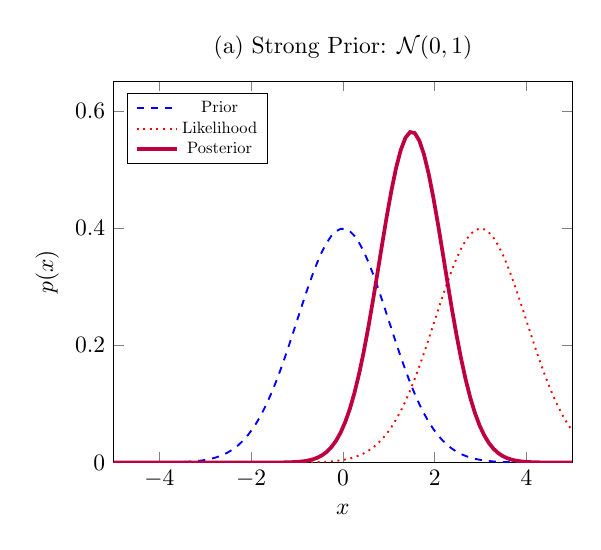
\begin{tikzpicture}[scale=0.85]
    \begin{axis}[
        title={(a) Strong Prior: $\mathcal{N}(0, 1)$},
        xlabel={$x$}, ylabel={$p(x)$},
        xmin=-5, xmax=5, ymin=0, ymax=0.65,
        domain=-5:5, samples=100,
        legend pos=north west, legend style={nodes={scale=0.7, transform shape}}
    ]
        % Prior: mean=0, var=1 (std=1)
        \addplot [blue, thick, dashed] {1/(1*sqrt(2*pi))*exp(-(x-0)^2/(2*1^2))};
        \addlegendentry{Prior}
        % Likelihood: mean=3, var=1 (std=1)
        \addplot [red, dotted, thick] {1/(1*sqrt(2*pi))*exp(-(x-3)^2/(2*1^2))};
        \addlegendentry{Likelihood}
        % Posterior: mean=1.5, var=0.5 (std=0.707)
        \addplot [purple, ultra thick] {1/(0.707*sqrt(2*pi))*exp(-(x-1.5)^2/(2*0.5))};
        \addlegendentry{Posterior}
    \end{axis}
    \end{tikzpicture}
\end{minipage}
\hfill
\begin{minipage}{0.48\textwidth}
    \centering
    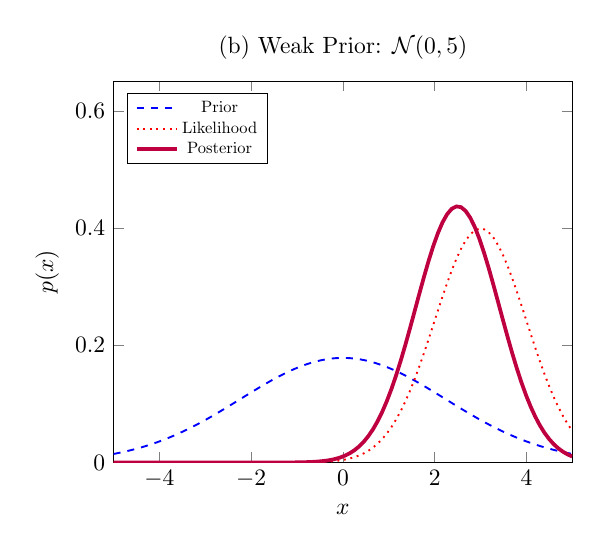
\begin{tikzpicture}[scale=0.85]
    \begin{axis}[
        title={(b) Weak Prior: $\mathcal{N}(0, 5)$},
        xlabel={$x$}, ylabel={$p(x)$},
        xmin=-5, xmax=5, ymin=0, ymax=0.65,
        domain=-5:5, samples=100,
        legend pos=north west, legend style={nodes={scale=0.7, transform shape}}
    ]
        % Prior: mean=0, var=5 (std=2.236)
        \addplot [blue, thick, dashed] {1/(2.236*sqrt(2*pi))*exp(-(x-0)^2/(2*5))};
        \addlegendentry{Prior}
        % Likelihood: mean=3, var=1 (std=1)
        \addplot [red, dotted, thick] {1/(1*sqrt(2*pi))*exp(-(x-3)^2/(2*1^2))};
        \addlegendentry{Likelihood}
        % Posterior: mean=2.5, var=0.833 (std=0.913)
        \addplot [purple, ultra thick] {1/(0.913*sqrt(2*pi))*exp(-(x-2.5)^2/(2*0.833))};
        \addlegendentry{Posterior}
    \end{axis}
    \end{tikzpicture}
\end{minipage}
\caption{Bayesian inference of an unknown state $z$ given a single observation $y=3$. In (a), the highly certain prior heavily shrinks the posterior mean toward 0. In (b), the weak prior allows the data to dominate the posterior result.}
\label{fig:gaussian_shrinkage}
\end{figure}

\subsection*{12.5. Signal-to-Noise Ratio (SNR)}
To cleanly formalize how trustworthy our underlying environment is compared to the corrupting noise, we define the \textbf{Signal-to-Noise Ratio (SNR)}:
\begin{equation}
\text{SNR} \triangleq \frac{\mathbb{E}[Z^2]}{\mathbb{E}[\epsilon^2]} = \frac{\Sigma_0 + \mu_0^2}{\Sigma_y} \tag{51}
\end{equation}
where $z \sim \mathcal{N}(\mu_0, \Sigma_0)$ represents our true structural signal energy, and $\epsilon \sim \mathcal{N}(0, \Sigma_y)$ represents the independent background white noise power. A massive SNR means our prior/signal properties dwarf the noise floor, leaving the posterior calculation exceptionally crisp.

\subsection*{12.6. Numerical Example: Multi-Sensor Scalar Inference and SNR}

To solidify how a sequence of noisy observations interacts with a prior and how to calculate the Signal-to-Noise Ratio (SNR) in practice, let's walk through a concrete numerical example using the exact equations derived above.

Imagine we are tracking the true voltage level $z$ of a battery cell. 
\begin{itemize}
    \item \textbf{Prior Setup:} Based on old manufacturing data, we expect the voltage to be around $\mu_0 = 0\text{V}$ (centered around a baseline nominal deviation), but we are highly uncertain. We assign a prior variance of $\Sigma_0 = \tau_0^2 = 4$, which gives us a prior precision of:
    \begin{equation*}
    \lambda_0 = \frac{1}{\Sigma_0} = \frac{1}{4} = 0.25
    \end{equation*}
    \item \textbf{Sensor/Likelihood Setup:} We hook up a cheap digital voltmeter to take readings. The sensor has a known measurement noise variance of $\Sigma_y = \sigma^2 = 2$. This gives the sensor a single-measurement precision of:
    \begin{equation*}
    \lambda_y = \frac{1}{\Sigma_y} = \frac{1}{2} = 0.5
    \end{equation*}
\end{itemize}

\subsubsection*{Step 1: Calculating the Signal-to-Noise Ratio (SNR)}
Before we even look at the incoming sensor data, we can evaluate the baseline quality of our physical environment using Equation (51):
\begin{equation}
\text{SNR} = \frac{\Sigma_0 + \mu_0^2}{\Sigma_y} = \frac{4 + 0^2}{2} = 2.0 \tag{52}
\end{equation}
An $\text{SNR} = 2.0$ tells us that the underlying signal variance (our potential true state space) is twice as large as the background thermal noise of the voltmeter. The data will carry clear structural information, but it still requires filtering.

\subsubsection*{Step 2: Processing the Incoming Stream ($N = 3$)}
Now, we turn on the voltmeter and take $N = 3$ consecutive readings back-to-back:
\begin{equation*}
y_1 = 3.5, \quad y_2 = 4.0, \quad y_3 = 4.5
\end{equation*}

First, we calculate the sample mean ($\bar{y}$), which represents the Maximum Likelihood Estimate (MLE) independent of our prior:
\begin{equation}
\bar{y} = \frac{1}{3}\sum_{i=1}^3 y_i = \frac{3.5 + 4.0 + 4.5}{3} = 4.0\text{V} \tag{53}
\end{equation}

\subsubsection*{Step 3: Finding the Total Posterior Precision and Variance}
Using Equation (46), we find our updated posterior precision $\lambda_N$ by accumulating our baseline prior certainty and the precision gathered from our 3 independent looks:
\begin{align}
\lambda_N &= \lambda_0 + N\lambda_y \nonumber \\
&= 0.25 + 3(0.5) = 0.25 + 1.50 = 1.75 \tag{54}
\end{align}

To view this back in terms of raw uncertainty/variance, we invert the final precision using Equation (56):
\begin{equation}
\tau_N^2 = \frac{1}{\lambda_N} = \frac{1}{1.75} = \frac{4}{7} \approx 0.571 \tag{55}
\end{equation}
Notice how our uncertainty collapsed drastically from our initial prior variance ($\Sigma_0 = 4$) and is even lower than the raw noise floor of a single sensor measurement ($\Sigma_y = 2$). 

\subsubsection*{Step 4: Finding the Posterior Mean via Convex Combination}
Now we look at where our final belief lands along the tracking line. Using Equation (47), we compute the weighted compromise:
\begin{align}
\mu_N &= \left( \frac{N\lambda_y}{\lambda_0 + N\lambda_y} \right)\bar{y} + \left( \frac{\lambda_0}{\lambda_0 + N\lambda_y} \right)\mu_0 \nonumber \\[0.5em]
&= \left( \frac{1.5}{1.75} \right)(4.0) + \left( \frac{0.25}{1.75} \right)(0) \tag{56}
\end{align}

Simplifying the fraction coefficients yields:
\begin{equation}
\mu_N = \left(\frac{6}{7}\right)(4.0) + \left(\frac{1}{7}\right)(0) = \frac{24}{7} \approx 3.428\text{V} \tag{57}
\end{equation}

\subsubsection*{Intuitive Takeaway}
Let's see what the math just did to our beliefs:
\begin{itemize}
    \item Our data told us the voltage looked like $4.0\text{V}$ ($\bar{y} = 4.0$).
    \item Our prior insisted the voltage was closer to $0\text{V}$ ($\mu_0 = 0$).
    \item Because we collected $3$ distinct observations, our total data information pool ($N\lambda_y = 1.5$) became exactly \textbf{6 times stronger} than our weak prior baseline ($\lambda_0 = 0.25$).
\end{itemize}
As a result, the posterior mean was pulled $\frac{6}{7}$ of the way toward the data, leaving us centered at $3.43\text{V}$. The remaining distance to $4.0\text{V}$ is the explicit effect of \textbf{prior shrinkage}—the system drags the raw data reading back toward zero slightly because it knows there is a chance the measurements were partially inflated by random positive noise.

\section*{13. Inferring an Unknown Vector}

When we transition from scalars to vectors, we are no longer just asking "how much noise is there?" We are also asking "\textbf{in which direction} is the noise pointing?" This section generalizes Bayesian inversion to multivariate systems, using a classic target-tracking scenario (like localizing an aircraft via radar blips) to illustrate the concepts.

\subsection*{13.1. Setting Up an Uninformative Vector Prior}
Let's assume we want to track an unknown 2D position vector $\mathbf{z} \in \mathbb{R}^2$. If we have absolutely no clue where the target is before we start tracking, we want an "infinitely wide" prior. 
\begin{equation}
\text{\textbf{Prior:}} \quad p(\mathbf{z}) = \mathcal{N}(\mathbf{z} \mid \boldsymbol{\mu}_z, \boldsymbol{\Sigma}_z) \tag{58}
\end{equation}

To mathematically state that we "know nothing," we set the prior mean to the origin and send the prior variance to infinity:
\begin{equation*}
\boldsymbol{\mu}_z = \mathbf{0}, \quad \boldsymbol{\Sigma}_z = \infty \mathbf{I} \implies \boldsymbol{\Sigma}_z^{-1} = \mathbf{0}
\end{equation*}
Setting the \textbf{prior precision} $\boldsymbol{\Sigma}_z^{-1}$ to zero means we place exactly zero weight or confidence on our initial guess.

\subsection*{13.2. The Sample Mean is a Sufficient Statistic}
Suppose we collect $N$ independent, noisy vector measurements $\mathbf{y}_n \sim \mathcal{N}(\mathbf{z}, \boldsymbol{\Sigma}_y)$. Multiplying all $N$ separate Gaussian distributions together looks messy, but a beautiful algebraic property allows us to compress the entire dataset down into a single averaged vector $\bar{\mathbf{y}}$:
\begin{equation}
p(\mathcal{D} \mid \mathbf{z}) = \prod_{n=1}^N \mathcal{N}(\mathbf{y}_n \mid \mathbf{z}, \boldsymbol{\Sigma}_y) \propto \mathcal{N}\left(\bar{\mathbf{y}} \ \middle|\ \mathbf{z}, \frac{1}{N}\boldsymbol{\Sigma}_y\right) \tag{59}
\end{equation}

To see why a cloud of data points shrinks the covariance matrix by $1/N$, let's look at the log-likelihood for just $2$ measurements ($\mathbf{y}_1$ and $\mathbf{y}_2$), keeping only the terms that interact with $\mathbf{z}$:
\begin{align*}
\ln\left(p(\mathbf{y}_1 \mid \mathbf{z})p(\mathbf{y}_2 \mid \mathbf{z})\right) &= -\frac{1}{2}\left[\mathbf{z}^T\boldsymbol{\Sigma}_y^{-1}\mathbf{z} - 2\mathbf{z}^T\boldsymbol{\Sigma}_y^{-1}\mathbf{y}_1\right] - \frac{1}{2}\left[\mathbf{z}^T\boldsymbol{\Sigma}_y^{-1}\mathbf{z} - 2\mathbf{z}^T\boldsymbol{\Sigma}_y^{-1}\mathbf{y}_2\right] + \text{const} \\
&= -\frac{1}{2}\left[ 2\mathbf{z}^T\boldsymbol{\Sigma}_y^{-1}\mathbf{z} - 2\mathbf{z}^T\boldsymbol{\Sigma}_y^{-1}(\mathbf{y}_1 + \mathbf{y}_2) \right] + \text{const}
\end{align*}

Let's factor out a $2$ to force the linear term to look like a sample mean $\bar{\mathbf{y}} = \frac{\mathbf{y}_1 + \mathbf{y}_2}{2}$:
\begin{align}
&= -\frac{1}{2}\left[ \mathbf{z}^T\left(2\boldsymbol{\Sigma}_y^{-1}\right)\mathbf{z} - 2\mathbf{z}^T\left(2\boldsymbol{\Sigma}_y^{-1}\right)\left(\frac{\mathbf{y}_1 + \mathbf{y}_2}{2}\right) \right] + \text{const} \tag{60} \\
&= -\frac{1}{2}\left[ \mathbf{z}^T\left(\frac{\boldsymbol{\Sigma}_y}{2}\right)^{-1}\mathbf{z} - 2\mathbf{z}^T\left(\frac{\boldsymbol{\Sigma}_y}{2}\right)^{-1}\bar{\mathbf{y}} \right] + \text{const} \tag{61}
\end{align}
Looking at the final coefficient, the precision doubled ($2\boldsymbol{\Sigma}_y^{-1}$), meaning our effective measurement covariance was sliced in half ($\boldsymbol{\Sigma}_y / 2$).

\subsection*{13.3. The Vector Bayes Update}
Now we substitute our compressed single-distribution likelihood into our linear Gaussian equations (setting $\mathbf{W} = \mathbf{I}$ and $\mathbf{b} = \mathbf{0}$):
\begin{equation}
\text{\textbf{Posterior:}} \quad p(\mathbf{z} \mid \mathbf{y}_1, \dots, \mathbf{y}_N) = \mathcal{N}(\mathbf{z} \mid \hat{\boldsymbol{\mu}}, \hat{\boldsymbol{\Sigma}}) \tag{62}
\end{equation}

\begin{equation}
\hat{\boldsymbol{\Sigma}}^{-1} = \boldsymbol{\Sigma}_z^{-1} + N\boldsymbol{\Sigma}_y^{-1} \tag{63}
\end{equation}

\begin{equation}
\hat{\boldsymbol{\mu}} = \hat{\boldsymbol{\Sigma}} \left( N\boldsymbol{\Sigma}_y^{-1}\bar{\mathbf{y}} + \boldsymbol{\Sigma}_z^{-1}\boldsymbol{\mu}_z \right) \tag{64}
\end{equation}

If we apply our "flat/uninformative" prior ($\boldsymbol{\Sigma}_z^{-1} = \mathbf{0}$), these equations collapse completely into the data metrics:
\begin{equation*}
\hat{\boldsymbol{\Sigma}} = \frac{1}{N}\boldsymbol{\Sigma}_y, \quad \hat{\boldsymbol{\mu}} = \bar{\mathbf{y}}
\end{equation*}

\subsection*{13.4. Visualizing Anisotropic Sensor Noise (Directional Uncertainty)}
When tracking a physical object, sensors often have different noise levels along different coordinate axes (\textbf{anisotropic noise}). Let's visualize a scenario where a radar sensor is highly precise along the vertical axis ($z_2$) but heavily blurred along the horizontal axis ($z_1$).

\begin{figure}[H]
\centering
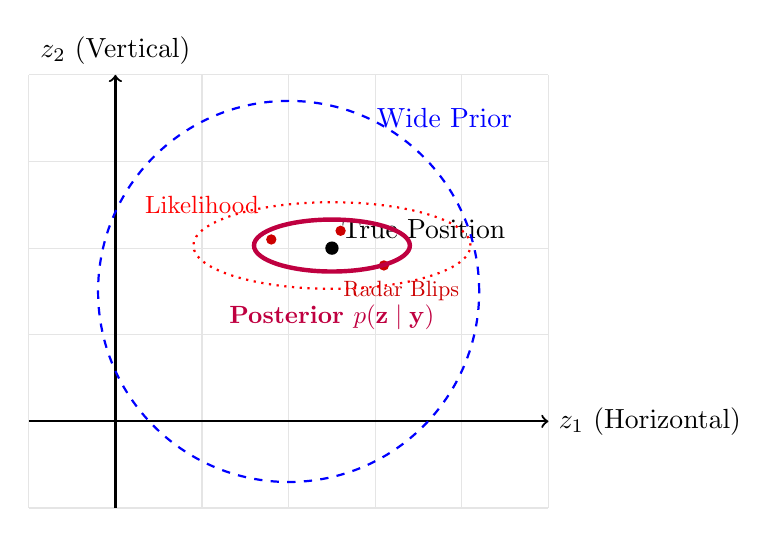
\begin{tikzpicture}[scale=1.1]
    % Grid lines for context
    \draw[black!10,step=1] (-1,-1) grid (5,4);
    \draw[->, thick] (-1,0) -- (5,0) node[right] {$z_1$ (Horizontal)};
    \draw[->, thick] (0,-1) -- (0,4) node[above] {$z_2$ (Vertical)};

    % True Position (Unknown to the system, but reference for us)
    \filldraw[black] (2.5, 2.0) circle (2pt) node[above right] {True Position};

    % Weak Prior (Huge wide circle representing complete uncertainty)
    \draw[blue, thick, dashed] (2, 1.5) circle (2.2cm);
    \node[blue] at (3.8, 3.5) {Wide Prior};

    % Individual Radar Blips (Observations)
    \filldraw[red!80!black] (1.8, 2.1) circle (1.5pt);
    \filldraw[red!80!black] (3.1, 1.8) circle (1.5pt);
    \filldraw[red!80!black] (2.6, 2.2) circle (1.5pt);
    \node[red!80!black, scale=0.8] at (3.3, 1.5) {Radar Blips};

    % Likelihood / Single measurement footprint (Wide horizontally, narrow vertically)
    % Center near the data average
    \draw[red, thick, dotted] (2.5, 2.03) ellipse (1.6cm and 0.5cm);
    \node[red, scale=0.9] at (1.0, 2.5) {Likelihood};

    % Posterior footprint (Tighter ellipse because multiple blips reduce variance)
    \draw[purple, ultra thick] (2.5, 2.03) ellipse (0.9cm and 0.3cm);
    \node[purple, font=\bfseries, scale=0.9] at (2.5, 1.2) {Posterior $p(\mathbf{z}\mid\mathbf{y})$};

\end{tikzpicture}
\caption{2D Localization with anisotropic measurement noise. Because the horizontal sensor channel is noisier than the vertical one, our posterior uncertainty retains an elongated elliptical shape, reflecting higher residual uncertainty along the $z_1$ axis.}
\label{fig:vector_localization}
\end{figure}

\subsection*{13.5. Numerical Example: 2D Radar Target Tracking}

To bring the multi-dimensional vector math down to earth, let's look at a concrete numerical example of tracking an aircraft's position vector $\mathbf{z} = [z_1, z_2]^T$ in a 2D space.

Let's define our starting parameters:
\begin{itemize}
    \item \textbf{Prior Setup:} We guess the target is near the origin $\boldsymbol{\mu}_z = \begin{bmatrix} 0 \\ 0 \end{bmatrix}$, with a prior covariance of $\boldsymbol{\Sigma}_z = \begin{bmatrix} 1 & 0 \\ 0 & 1 \end{bmatrix}$. This means our initial prior precision matrix is:
    \begin{equation*}
    \boldsymbol{\Sigma}_z^{-1} = \begin{bmatrix} 1 & 0 \\ 0 & 1 \end{bmatrix}
    \end{equation*}
    \item \textbf{Sensor/Likelihood Setup:} Our radar sensor is anisotropic—it is twice as accurate vertically as it is horizontally. Its single-measurement noise covariance is $\boldsymbol{\Sigma}_y = \begin{bmatrix} 1 & 0 \\ 0 & 0.5 \end{bmatrix}$. Inverting this gives us our sensor precision matrix (information density):
    \begin{equation*}
    \boldsymbol{\Sigma}_y^{-1} = \begin{bmatrix} 1 & 0 \\ 0 & 2 \end{bmatrix}
    \end{equation*}
\end{itemize}

Now, suppose the radar records $N = 2$ rapid blips:
\begin{equation*}
\mathbf{y}_1 = \begin{bmatrix} 4 \\ 4.8 \end{bmatrix}, \quad \mathbf{y}_2 = \begin{bmatrix} 2 \\ 5.2 \end{bmatrix}
\end{equation*}

Let's compute our updated spatial belief step-by-step.

\paragraph{Step 1: Compute the Dataset Sample Mean}
Using Equation (59), we compress our two radar blips into their average vector position ($\bar{\mathbf{y}}$):
\begin{equation}
\bar{\mathbf{y}} = \frac{\mathbf{y}_1 + \mathbf{y}_2}{2} = \frac{1}{2} \left( \begin{bmatrix} 4 \\ 4.8 \end{bmatrix} + \begin{bmatrix} 2 \\ 5.2 \end{bmatrix} \right) = \begin{bmatrix} 3 \\ 5 \end{bmatrix} \tag{65}
\end{equation}

\paragraph{Step 2: Compute the Posterior Precision Matrix $\hat{\boldsymbol{\Sigma}}^{-1}$}
Using Equation (63), we sum our baseline prior confidence with the total information harvested from our $2$ observations:
\begin{align}
\hat{\boldsymbol{\Sigma}}^{-1} &= \boldsymbol{\Sigma}_z^{-1} + N\boldsymbol{\Sigma}_y^{-1} \nonumber \\
&= \begin{bmatrix} 1 & 0 \\ 0 & 1 \end{bmatrix} + 2\begin{bmatrix} 1 & 0 \\ 0 & 2 \end{bmatrix} \nonumber \\
&= \begin{bmatrix} 1 & 0 \\ 0 & 1 \end{bmatrix} + \begin{bmatrix} 2 & 0 \\ 0 & 4 \end{bmatrix} = \begin{bmatrix} 3 & 0 \\ 0 & 5 \end{bmatrix} \tag{66}
\end{align}

\paragraph{Step 3: Compute the Posterior Covariance Matrix $\hat{\boldsymbol{\Sigma}}$}
To find our updated spatial uncertainty footprint, we take the inverse of our new precision matrix:
\begin{equation}
\hat{\boldsymbol{\Sigma}} = \begin{bmatrix} 3 & 0 \\ 0 & 5 \end{bmatrix}^{-1} = \begin{bmatrix} \frac{1}{3} & 0 \\ 0 & \frac{1}{5} \end{bmatrix} = \begin{bmatrix} 0.333 & 0 \\ 0 & 0.200 \end{bmatrix} \tag{67}
\end{equation}
Notice that our uncertainty shrunk in both directions, but it shrunk \textbf{more vertically} (variance dropped from $1 \to 0.2$) than horizontally (variance dropped from $1 \to 0.333$) because the radar sensor passes higher quality data along the vertical tracking channel.

\paragraph{Step 4: Compute the Posterior Mean Vector $\hat{\boldsymbol{\mu}}$}
Finally, we apply Equation (64) to calculate our absolute best guess for the aircraft's current coordinate coordinates:
\begin{equation*}
\hat{\boldsymbol{\mu}} = \hat{\boldsymbol{\Sigma}} \left( N\boldsymbol{\Sigma}_y^{-1}\bar{\mathbf{y}} + \boldsymbol{\Sigma}_z^{-1}\boldsymbol{\mu}_z \right)
\end{equation*}

Let's plug in our known matrix pieces and multiply them out:
\begin{align}
\hat{\boldsymbol{\mu}} &= \begin{bmatrix} \frac{1}{3} & 0 \\ 0 & \frac{1}{5} \end{bmatrix} \left( \begin{bmatrix} 2 & 0 \\ 0 & 4 \end{bmatrix}\begin{bmatrix} 3 \\ 5 \end{bmatrix} + \begin{bmatrix} 1 & 0 \\ 0 & 1 \end{bmatrix}\begin{bmatrix} 0 \\ 0 \end{bmatrix} \right) \nonumber \\
&= \begin{bmatrix} \frac{1}{3} & 0 \\ 0 & \frac{1}{5} \end{bmatrix} \left( \begin{bmatrix} 6 \\ 20 \end{bmatrix} + \begin{bmatrix} 0 \\ 0 \end{bmatrix} \right) \nonumber \\
&= \begin{bmatrix} \frac{1}{3} \cdot 6 \\ \frac{1}{5} \cdot 20 \end{bmatrix} = \begin{bmatrix} 2 \\ 4 \end{bmatrix} \tag{68}
\end{align}

\paragraph{Analysis of the Results}
Look at how our final coordinates $\hat{\boldsymbol{\mu}} = [2, 4]^T$ balance the data and prior:
\begin{itemize}
    \item \textbf{Horizontal Component ($z_1$):} The prior wanted $0$, the data average was $3$. Because the horizontal radar channel was moderately noisy, the prior pulled the estimate back to $2$ (\textit{a shrinkage effect of $-1.0$}).
    \item \textbf{Vertical Component ($z_2$):} The prior wanted $0$, the data average was $5$. Because the vertical radar channel was highly precise, the data dominated the update, dragging our belief all the way up to $4$ (\textit{a shrinkage effect of only $-1.0$ despite a much larger gap}).
\end{itemize}
This demonstrates how multivariate Gaussian equations automatically calculate directional compromises based entirely on the shape of your measurement noise.

\section*{14. Sensor Fusion}

In the real world, an autonomous robot or an autopilot system never relies on just one sensor. It might look at a camera, a radar, and an IMU simultaneously. Each of these sensors has different strengths, weaknesses, and levels of reliability. 

**Sensor Fusion** is the mathematical process of combining measurements from multiple distinct hardware devices to produce an ultimate state estimate that is more accurate than any single sensor could achieve on its own.

\subsection*{14.1. Stacking Multiple Sensors into a Single Matrix}
Let's look at a 2D space where a hidden state $\mathbf{z}$ is observed by $M$ different sensors. Each sensor $m$ takes $N_m$ independent readings. The joint distribution of this entire system can be written as:
\begin{equation}
p(\mathbf{z}, \mathbf{y}) = p(\mathbf{z}) \prod_{m=1}^M \prod_{n=1}^{N_m} \mathcal{N}(\mathbf{y}_{n,m} \mid \mathbf{z}, \boldsymbol{\Sigma}_m) \tag{69}
\end{equation}

To understand how to solve this cleanly, let's look at the foundational case of exactly **two sensors** taking a single simultaneous reading:
\begin{align*}
\text{Sensor 1:} \quad \mathbf{y}_1 &\sim \mathcal{N}(\mathbf{z}, \boldsymbol{\Sigma}_1) \\
\text{Sensor 2:} \quad \mathbf{y}_2 &\sim \mathcal{N}(\mathbf{z}, \boldsymbol{\Sigma}_2)
\end{align*}

Pictorially, this is a generative branching tree: $\mathbf{y}_1 \leftarrow \mathbf{z} \rightarrow \mathbf{y}_2$. To solve this using our standard linear Gaussian identities, we use a brilliant matrix packing trick. We stack both observations into a single joint vector $\mathbf{y}$ and group the independent noise profiles into a giant **block-diagonal covariance matrix**:

\begin{equation}
\mathbf{y} = \begin{bmatrix} \mathbf{y}_1 \\ \mathbf{y}_2 \end{bmatrix}, \quad \mathbf{W} = \begin{bmatrix} \mathbf{I} \\ \mathbf{I} \end{bmatrix}, \quad \boldsymbol{\Sigma}_y = \begin{bmatrix} \boldsymbol{\Sigma}_1 & \mathbf{0} \\ \mathbf{0} & \boldsymbol{\Sigma}_2 \end{bmatrix} \tag{70}
\end{equation}

By formatting the parameters this way, our multi-sensor problem collapses back into a standard linear model: $p(\mathbf{y} \mid \mathbf{z}) = \mathcal{N}(\mathbf{y} \mid \mathbf{W}\mathbf{z}, \boldsymbol{\Sigma}_y)$. We can now use standard Bayesian inversion to read off the fused posterior parameters directly.

\subsection*{14.2. The Intuitive Geometries of Fusion}
When you fuse two sensors together, three fascinating geometric behaviors emerge depending on the structural layout of the noise matrices $\boldsymbol{\Sigma}_1$ and $\boldsymbol{\Sigma}_2$. Let's break them down:

\begin{enumerate}
    \item \textbf{Equal Reliability (Isotropic Homogeneity):} If $\boldsymbol{\Sigma}_1 = \boldsymbol{\Sigma}_2$, both sensors are identical copies. The system plays a perfectly balanced game of tug-of-war, placing the fused posterior mean \textbf{exactly halfway} between the two data points.
    \item \textbf{Unequal Reliability (Isotropic Heterogeneity):} If Sensor 2 has significantly lower variance than Sensor 1 ($\boldsymbol{\Sigma}_2 < \boldsymbol{\Sigma}_1$), the system dynamically senses that Sensor 2 is cleaner. The posterior mean gets strongly \textbf{pulled toward $\mathbf{y}_2$}, mostly ignoring the noisy $\mathbf{y}_1$.
    \item \textbf{Directional / Anisotropic Reliability (The Superpower of Matrix Fusion):} Suppose Sensor 1 has low vertical variance but terrible horizontal variance. Conversely, suppose Sensor 2 has low horizontal variance but terrible vertical variance. 
    
    The matrix machinery acts like an automated optimal selector: it extracts the pristine vertical tracking from Sensor 1 and couples it with the pristine horizontal tracking from Sensor 2. The resulting fused posterior is **more accurate than both sensors across every single axis**.
\end{enumerate}

\subsection*{14.3. Visualizing the Three Fusion Scenarios}
The TikZ plots below demonstrate exactly how the posterior calculation behaves under these three distinct noise profiles, tracking two sensor blips located at $\mathbf{y}_1 = (1,3)$ and $\mathbf{y}_2 = (3,1)$.

\begin{figure}[H]
\centering
% Scenario A
\begin{minipage}{0.32\textwidth}
    \centering
    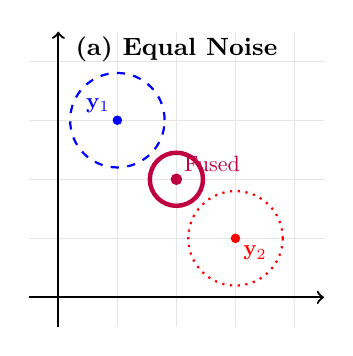
\begin{tikzpicture}[scale=0.75]
        \draw[black!10,step=1] (-0.5,-0.5) grid (4.5,4.5);
        \draw[->, thick] (-0.5,0) -- (4.5,0);
        \draw[->, thick] (0,-0.5) -- (0,4.5);
        \node[font=\small\bfseries] at (2,4.2) {(a) Equal Noise};
        
        % Sensor 1
        \filldraw[blue] (1,3) circle (2pt) node[above left, scale=0.8] {$\mathbf{y}_1$};
        \draw[blue, thick, dashed] (1,3) circle (0.8cm);
        % Sensor 2
        \filldraw[red] (3,1) circle (2pt) node[below right, scale=0.8] {$\mathbf{y}_2$};
        \draw[red, thick, dotted] (3,1) circle (0.8cm);
        % Posterior
        \filldraw[purple] (2,2) circle (2.5pt) node[above right, scale=0.8] {Fused};
        \draw[purple, ultra thick] (2,2) circle (0.45cm);
    \end{tikzpicture}
\end{minipage}
\hfill
% Scenario B
\begin{minipage}{0.32\textwidth}
    \centering
    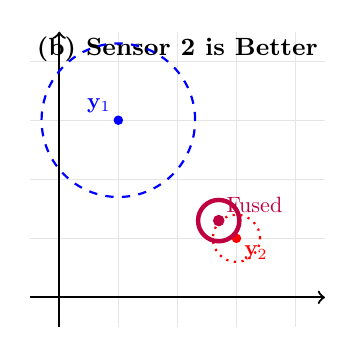
\begin{tikzpicture}[scale=0.75]
        \draw[black!10,step=1] (-0.5,-0.5) grid (4.5,4.5);
        \draw[->, thick] (-0.5,0) -- (4.5,0);
        \draw[->, thick] (0,-0.5) -- (0,4.5);
        \node[font=\small\bfseries] at (2,4.2) {(b) Sensor 2 is Better};
        
        % Sensor 1 (Noisy)
        \filldraw[blue] (1,3) circle (2pt) node[above left, scale=0.8] {$\mathbf{y}_1$};
        \draw[blue, thick, dashed] (1,3) circle (1.3cm);
        % Sensor 2 (Clean)
        \filldraw[red] (3,1) circle (2pt) node[below right, scale=0.8] {$\mathbf{y}_2$};
        \draw[red, thick, dotted] (3,1) circle (0.4cm);
        % Posterior (Pulled near y2)
        \filldraw[purple] (2.7,1.3) circle (2.5pt) node[above right, scale=0.8] {Fused};
        \draw[purple, ultra thick] (2.7,1.3) circle (0.35cm);
    \end{tikzpicture}
\end{minipage}
\hfill
% Scenario C
\begin{minipage}{0.32\textwidth}
    \centering
    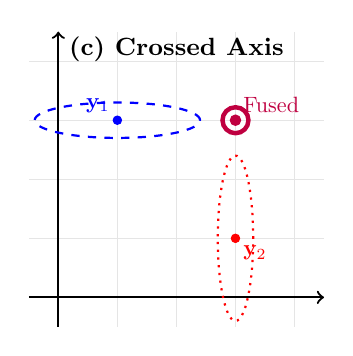
\begin{tikzpicture}[scale=0.75]
        \draw[black!10,step=1] (-0.5,-0.5) grid (4.5,4.5);
        \draw[->, thick] (-0.5,0) -- (4.5,0);
        \draw[->, thick] (0,-0.5) -- (0,4.5);
        \node[font=\small\bfseries] at (2,4.2) {(c) Crossed Axis};
        
        % Sensor 1 (Wide horizontally, tight vertically)
        \filldraw[blue] (1,3) circle (2pt) node[above left, scale=0.8] {$\mathbf{y}_1$};
        \draw[blue, thick, dashed] (1,3) ellipse (1.4cm and 0.3cm);
        % Sensor 2 (Tight horizontally, wide vertically)
        \filldraw[red] (3,1) circle (2pt) node[below right, scale=0.8] {$\mathbf{y}_2$};
        \draw[red, thick, dotted] (3,1) ellipse (0.3cm and 1.4cm);
        % Posterior (Intersects perfectly at the crosshair intersection coordinate)
        \filldraw[purple] (3,3) circle (2.5pt) node[above right, scale=0.8] {Fused};
        \draw[purple, ultra thick] (3,3) circle (0.22cm);
    \end{tikzpicture}
\end{minipage}
\caption{Three distinct environments for 2D Sensor Fusion. In (a), the estimate splits the difference. In (b), the cleaner sensor dominates. In (c), the system cherry-picks the cleanest directional tracking axis from each individual sensor, resulting in an exceptionally tight intersection profile centered at $(3,3)$.}
\label{fig:sensor_fusion_cases}
\end{figure}

\subsection*{14.4. Numerical Example: Fusing Complementary Heterogeneous Sensors}

To see the true mathematical "superpower" of multi-sensor fusion, let's work through a numerical example representing **Scenario (c)**, where two sensors have crossed, complementary accuracy axes.

Imagine an autonomous delivery drone trying to determine its 2D position vector $\mathbf{z} = [z_1, z_2]^T$. It takes readings from two different onboard systems simultaneously:
\begin{itemize}
    \item \textbf{Sensor 1 (Laser Rangefinder):} Exceptional at vertical distance tracking, but terrible at horizontal tracking. Its noise covariance is $\boldsymbol{\Sigma}_1 = \begin{bmatrix} 0.1 & 0 \\ 0 & 0.01 \end{bmatrix}$, yielding a precision matrix of:
    \begin{equation*}
    \boldsymbol{\Sigma}_1^{-1} = \begin{bmatrix} 10 & 0 \\ 0 & 100 \end{bmatrix}
    \end{equation*}
    \item \textbf{Sensor 2 (Computer Vision Odometer):} Exceptional at horizontal tracking, but terrible at vertical depth. Its noise covariance is $\boldsymbol{\Sigma}_2 = \begin{bmatrix} 0.01 & 0 \\ 0 & 0.1 \end{bmatrix}$, yielding a precision matrix of:
    \begin{equation*}
    \boldsymbol{\Sigma}_2^{-1} = \begin{bmatrix} 100 & 0 \\ 0 & 10 \end{bmatrix}
    \end{equation*}
\end{itemize}

To keep the focus entirely on how these two sensors blend together, we will assume a flat, uninformative spatial prior ($\boldsymbol{\Sigma}_z^{-1} = \mathbf{0}$). 

At a specific time step, the two sensors register the following conflicting blips:
\begin{equation*}
\mathbf{y}_1 = \begin{bmatrix} 1 \\ 3 \end{bmatrix}, \quad \mathbf{y}_2 = \begin{bmatrix} 3 \\ 1 \end{bmatrix}
\end{equation*}

Let's compute the fused posterior step-by-step.

\paragraph{Step 1: Compute the Fused Posterior Precision Matrix $\hat{\boldsymbol{\Sigma}}^{-1}$}
Information updates by straightforward addition. We sum the precision matrices of both hardware devices to calculate the total system certainty:
\begin{align}
\hat{\boldsymbol{\Sigma}}^{-1} &= \boldsymbol{\Sigma}_z^{-1} + \boldsymbol{\Sigma}_1^{-1} + \boldsymbol{\Sigma}_2^{-1} \nonumber \\
&= \begin{bmatrix} 0 & 0 \\ 0 & 0 \end{bmatrix} + \begin{bmatrix} 10 & 0 \\ 0 & 100 \end{bmatrix} + \begin{bmatrix} 100 & 0 \\ 0 & 10 \end{bmatrix} = \begin{bmatrix} 110 & 0 \\ 0 & 110 \end{bmatrix} \tag{71}
\end{align}

\paragraph{Step 2: Compute the Fused Posterior Covariance Matrix $\hat{\boldsymbol{\Sigma}}$}
To find our ultimate spatial uncertainty footprint, we invert the total precision matrix:
\begin{equation}
\hat{\boldsymbol{\Sigma}} = \begin{bmatrix} 110 & 0 \\ 0 & 110 \end{bmatrix}^{-1} = \begin{bmatrix} \frac{1}{110} & 0 \\ 0 & \frac{1}{110} \end{bmatrix} \approx \begin{bmatrix} 0.009 & 0 \\ 0 & 0.009 \end{bmatrix} \tag{72}
\end{equation}
Look at how spectacular this result is! The final variance along \textit{both} axes ($\approx 0.009$) is lower than the best single axis of either individual sensor ($0.01$). By combining them, the drone is now more certain of its location than either sensor could ever claim individually.

\paragraph{Step 3: Compute the Fused Information Vectors}
Next, we calculate the individual information vectors ($\boldsymbol{\Sigma}_m^{-1}\mathbf{y}_m$), which scale the raw measurements by their respective directional confidence weights:
\begin{align}
\text{\textbf{Sensor 1 Vector:}} \quad \boldsymbol{\Sigma}_1^{-1}\mathbf{y}_1 &= \begin{bmatrix} 10 & 0 \\ 0 & 100 \end{bmatrix} \begin{bmatrix} 1 \\ 3 \end{bmatrix} = \begin{bmatrix} 10 \\ 300 \end{bmatrix} \tag{73} \\
\text{\textbf{Sensor 2 Vector:}} \quad \boldsymbol{\Sigma}_2^{-1}\mathbf{y}_2 &= \begin{bmatrix} 100 & 0 \\ 0 & 10 \end{bmatrix} \begin{bmatrix} 3 \\ 1 \end{bmatrix} = \begin{bmatrix} 300 \\ 10 \end{bmatrix} \tag{74}
\end{align}
Notice how Sensor 1's vertical component shoots up to $300$ because it is highly trusted, while its horizontal component is muted down to $10$. Sensor 2 exhibits the exact opposite behavior.

\paragraph{Step 4: Calculate the Ultimate Fused Coordinate Mean $\hat{\boldsymbol{\mu}}$}
We sum the information vectors and multiply them by our fused covariance matrix:
\begin{align}
\hat{\boldsymbol{\mu}} &= \hat{\boldsymbol{\Sigma}} \left( \boldsymbol{\Sigma}_1^{-1}\mathbf{y}_1 + \boldsymbol{\Sigma}_2^{-1}\mathbf{y}_2 \right) \nonumber \\
&= \begin{bmatrix} \frac{1}{110} & 0 \\ 0 & \frac{1}{110} \end{bmatrix} \left( \begin{bmatrix} 10 \\ 300 \end{bmatrix} + \begin{bmatrix} 300 \\ 10 \end{bmatrix} \right) \nonumber \\
&= \begin{bmatrix} \frac{1}{110} & 0 \\ 0 & \frac{1}{110} \end{bmatrix} \begin{bmatrix} 310 \\ 310 \end{bmatrix} = \begin{bmatrix} \frac{310}{110} \\ \frac{310}{110} \end{bmatrix} = \begin{bmatrix} 2.818 \\ 2.818 \end{bmatrix} \tag{75}
\end{align}

\paragraph{Intuitive Engineering Takeaway}
Let's analyze why our final coordinates landed at exactly $(2.82, 2.82)$:
\begin{itemize}
    \item \textbf{Horizontal Axis ($z_1$):} Sensor 1 said $1$, Sensor 2 said $3$. Because Sensor 2 was 10 times more precise horizontally ($\lambda=100$ vs $\lambda=10$), the fused mean was pulled $\frac{10}{11}$ of the way toward Sensor 2's claim, locking in tightly at $2.82$.
    \item \textbf{Vertical Axis ($z_2$):} Sensor 1 said $3$, Sensor 2 said $1$. Because Sensor 1 was 10 times more precise vertically ($\lambda=100$ vs $\lambda=10$), the fused mean was pulled $\frac{10}{11}$ of the way toward Sensor 1's claim, locking in tightly at $2.82$.
\end{itemize}

The Kalman filtering machinery automatically managed this matrix handshake behind the scenes. It cherry-picked the pristine horizontal data from Sensor 2 and combined it with the pristine vertical data from Sensor 1, creating a highly precise, unified target estimation.

\section*{15. The Exponential Family}

In statistics and machine learning, we encounter dozens of different probability distributions: Gaussian, Bernoulli, Poisson, Gamma, Beta, and Multinomial. Tracking separate mathematical rules for each one is exhausting. 

The \textbf{Exponential Family} is a universal mathematical template. It turns out that almost all common clean distributions are just the exact same equation wearing different disguises. If we can prove a property holds true for this single template, we instantly prove it for all of them simultaneously.

\subsection*{15.1. The Master Template Equation}
A probability distribution belongs to the exponential family if its probability density function can be refactored to look exactly like this:

\begin{equation}
p(y \mid \boldsymbol{\eta}) = \frac{1}{Z(\boldsymbol{\eta})} h(y) \exp\left[ \boldsymbol{\eta}^T \mathbf{T}(y) \right] \tag{76}
\end{equation}

By moving the normalizing term $Z(\boldsymbol{\eta})$ into the exponent as a logarithm, we get the more common, elegant canonical format:
\begin{equation}
p(y \mid \boldsymbol{\eta}) = h(y) \exp\left[ \boldsymbol{\eta}^T \mathbf{T}(y) - A(\boldsymbol{\eta}) \right] \tag{77}
\end{equation}

Let's strip away the intimidating notation and define the 4 essential components of this template:
\begin{itemize}
    \item $\mathbf{T}(y) \in \mathbb{R}^K$ --- \textbf{The Sufficient Statistics}: This is a compression function for your data. It extracts every drop of useful information from a data point $y$ needed to estimate parameters. For a Gaussian, it extracts $y$ and $y^2$. Once you have $\mathbf{T}(y)$, you can throw the raw data away without losing information.
    \item $\boldsymbol{\eta} \in \mathbb{R}^K$ --- \textbf{The Natural (or Canonical) Parameters}: These are the fundamental mathematical "knobs" of the distribution. They aren't always the standard parameters we talk about (like a Gaussian mean $\mu$ or variance $\sigma^2$), but they are the mathematically cleaner forms that control the system linearly.
    \item $h(y)$ --- \textbf{The Base Measure}: A baseline scaling factor that usually serves to normalize the raw data space. In many common distributions, this is simply equal to $1$.
    \item $A(\boldsymbol{\eta}) = \ln Z(\boldsymbol{\eta})$ --- \textbf{The Log Partition Function}: This is the traffic cop of the distribution. Its primary job is to act as a normalizer to ensure the total probability integrates perfectly to $1.0$. 
    
    \textit{The Magic Trick of $A(\boldsymbol{\eta})$:} In advanced machine learning, calculating expectations (means and variances) requires solving difficult calculus integrals. If a distribution is in the exponential family, you can skip integrals entirely! Differentiating $A(\boldsymbol{\eta})$ once gives you the exact mean of the distribution, and differentiating it twice gives you the variance.
\end{itemize}

\subsection*{15.2. Visualizing the Unified Ecosystem}
Think of the Exponential Family as an umbrella ecosystem. By simply swapping out what we choose for $\boldsymbol{\eta}$ and $\mathbf{T}(y)$, the exact same template equation transforms into entirely different distributions.

\begin{figure}[H]
\centering
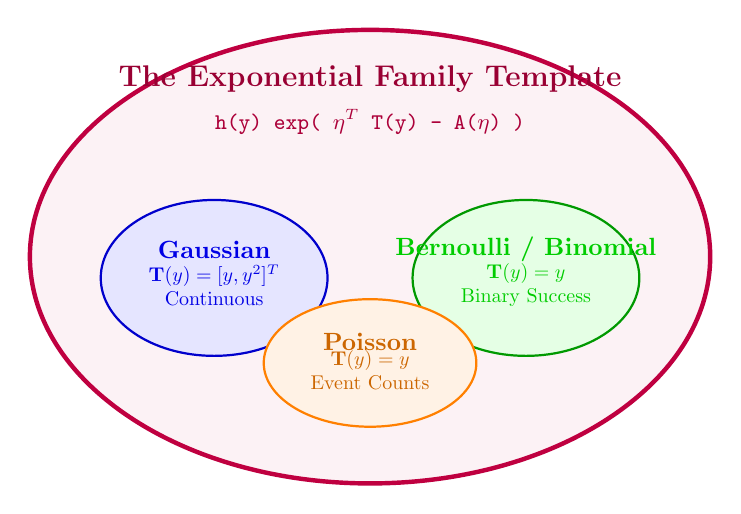
\begin{tikzpicture}[scale=0.9, every node/.style={transform shape}]
    % Giant Master Template Bubble
    \draw[purple, ultra thick, fill=purple!5] (0,0) ellipse (4.8cm and 3.2cm);
    \node[purple!80!black, font=\large\bfseries] at (0, 2.5) {The Exponential Family Template};
    \node[purple!90!black, font=\ttfamily\small] at (0, 1.9) {h(y) exp( $\eta^T$ T(y) - A($\eta$) )};

    % Child Distributions
    % Gaussian
    \draw[blue!80!black, thick, fill=blue!10] (-2.2, -0.3) ellipse (1.6cm and 1.1cm);
    \node[blue!90!black, font=\bfseries] at (-2.2, 0.1) {Gaussian};
    \node[blue!90!black, scale=0.8, align=center] at (-2.2, -0.4) {$\mathbf{T}(y) = [y, y^2]^T$ \\ Continuous};

    % Bernoulli
    \draw[green!60!black, thick, fill=green!10] (2.2, -0.3) ellipse (1.6cm and 1.1cm);
    \node[green!80!black, font=\bfseries] at (2.2, 0.1) {Bernoulli / Binomial};
    \node[green!80!black, scale=0.8, align=center] at (2.2, -0.4) {$\mathbf{T}(y) = y$ \\ Binary Success};

    % Poisson
    \draw[orange, thick, fill=orange!10] (0, -1.5) ellipse (1.5cm and 0.9cm);
    \node[orange!80!black, font=\bfseries] at (0, -1.2) {Poisson};
    \node[orange!80!black, scale=0.8, align=center] at (0, -1.6) {$\mathbf{T}(y) = y$ \\ Event Counts};
\end{tikzpicture}
\caption{Conceptual map of the Exponential Family ecosystem. Despite looking radically different in standard textbooks, Gaussians, Bernoullis, and Poissons are structurally identical underneath their notation.}
\label{fig:exponential_family_map}
\end{figure}

\subsection*{15.3. Subtypes and Variations}
Depending on how the knobs are wired, we categorize the family into three major structural flavors:

\begin{enumerate}
    \item \textbf{Minimal Exponential Family:} A setup where every single parameter knob in $\boldsymbol{\eta}$ is completely independent of the others. There are no redundant variables or constraints. (If a distribution has a constraint, like a Multinomial where probabilities must add up to $1$, it is \textit{non-minimal}, but we can easily fix it by throwing away one redundant dimension).
    
    \item \textbf{Curved Exponential Family:} Sometimes, the true physical parameters $\boldsymbol{\phi}$ map onto our natural parameters via a non-linear function: $\boldsymbol{\eta} = f(\boldsymbol{\phi})$. If $f$ is non-linear, the parameter space curves like a geometric sheet. This happens when the mean and variance of a system are rigidly locked to one another by a shared physical constraint.
    
    \item \textbf{Natural Exponential Family (NEF):} The absolute simplest variation of the template. A distribution is "Natural" if the sufficient statistic function does nothing to the data at all: 
    \begin{equation*}
    \mathbf{T}(y) = y
    \end{equation*}
    When this happens, the equation condenses into a clean inner product between the parameter vector and raw data vector:
    \begin{equation}
    p(y \mid \boldsymbol{\eta}) = h(y) \exp\left[ \boldsymbol{\eta}^T y - A(\boldsymbol{\eta}) \right] \tag{78}
    \end{equation}
    Distributions like the Bernoulli and Poisson live directly inside this highly prized NEF territory.
\end{enumerate}

\section*{16. Concrete Example: The Bernoulli Distribution and Cumulants}

To see how the abstract exponential family template works in real life, let's dissect the simplest distribution in existence: the \textbf{Bernoulli distribution} (a single biased coin flip where $y=1$ is heads and $y=0$ is tails). 

We will see how rearranging this distribution exposes a secret bridge to neural networks (the Sigmoid function) and unlocks a mathematical cheat code for finding means and variances without doing calculus integration.

\subsection*{16.1. The Over-Complete Disguise}
The standard way to write the probability of a Bernoulli event with success probability $\mu$ is:
\begin{equation}
p(y \mid \mu) = \mu^y (1 - \mu)^{1-y} \tag{79}
\end{equation}

To force this into our exponential family template, we apply an old algebraic trick: slide the whole expression into an exponential and log block ($\alpha = e^{\ln \alpha}$):
\begin{align}
p(y \mid \mu) &= \exp\left[ \ln\left( \mu^y (1 - \mu)^{1-y} \right) \right] \nonumber \\
&= \exp\left[ y \ln(\mu) + (1 - y) \ln(1 - \mu) \right] \tag{80}
\end{align}

If we try to match this directly to our template ($\exp[\boldsymbol{\eta}^T \mathbf{T}(y)]$), we get:
\begin{equation*}
\mathbf{T}(y) = \begin{bmatrix} y \\ 1-y \end{bmatrix}, \quad \boldsymbol{\eta} = \begin{bmatrix} \ln(\mu) \\ \ln(1-\mu) \end{bmatrix}
\end{equation*}

This is called an \textbf{over-complete representation}. Why? Because the two components of our data features are hard-locked by a rigid linear dependency: $y + (1-y) = 1$ always! Because the data components are redundant, the parameter knobs in $\boldsymbol{\eta}$ are not uniquely identifiable. There are infinitely many combinations of parameters that produce identical probabilities, causing optimization algorithms to wander aimlessly.

\subsection*{16.2. Striping Redundancy: The Minimal Representation}
To fix this, we use basic algebra to compress the exponent down to a single independent term involving $y$:
\begin{align}
y \ln(\mu) + (1 - y) \ln(1 - \mu) &= y \ln(\mu) + \ln(1 - \mu) - y \ln(1 - \mu) \nonumber \\
&= y \left( \ln(\mu) - \ln(1 - \mu) \right) + \ln(1 - \mu) \nonumber \\
&= y \ln\left( \frac{\mu}{1 - \mu} \right) + \ln(1 - \mu) \tag{81}
\end{align}

Now, let's slide this back into the exponential function. The Bernoulli distribution is now perfectly optimized in its unique, \textbf{minimal representation}:
\begin{equation}
p(y \mid \mu) = \exp\left[ y \ln\left( \frac{\mu}{1 - \mu} \right) + \ln(1 - \mu) \right] \tag{82}
\end{equation}

\subsection*{16.3. Reading Off the Template Variables}
Now we can cleanly map Equation (82) directly to our master template ($h(y) \exp[\eta T(y) - A(\eta)]$). The match is beautiful:
\begin{itemize}
    \item $h(y) = 1$ (The base measure is trivial).
    \item $T(y) = y$ (The sufficient statistic is just the raw data value itself).
    \item $\eta = \ln\left( \frac{\mu}{1 - \mu} \right)$ --- \textbf{The Natural Parameter}: This is the standard log-odds or \textbf{logit} function from logistic regression.
    \item $A(\eta) = -\ln(1 - \mu)$ --- \textbf{The Log Partition Function}: To write this purely in terms of our natural parameter $\eta$, we invert the logit function to express $\mu$ in terms of $\eta$:
    \begin{equation}
    \mu = \frac{1}{1 + e^{-\eta}} = \sigma(\eta) \tag{83}
    \end{equation}
\end{itemize}
This is the famous \textbf{Logistic Sigmoid function}! This is why logistic regression and neural networks use the sigmoid function for binary classification—the math is forced upon us by the underlying physics of the exponential family.

Substituting $\mu = \sigma(\eta)$ back into $A(\eta)$ yields its final, canonical parameter form:
\begin{equation}
A(\eta) = -\ln\left(1 - \frac{1}{1 + e^{-\eta}}\right) = -\ln\left(\frac{e^{-\eta}}{1 + e^{-\eta}}\right) = \ln(1 + e^{\eta}) \tag{84}
\end{equation}

\subsection*{16.4. The Magic Cheat Code: Generating Cumulants}
As stated in Section 15, calculating moments (like the mean and variance) usually requires solving calculus integrals or sums: $\mathbb{E}[Y] = \sum y \cdot p(y)$. 

But for an exponential family distribution, the log partition function $A(\eta) = \ln(1 + e^{\eta})$ acts as a \textbf{cumulant generating function}. We can bypass standard probability calculations entirely by taking simple derivatives with respect to $\eta$.

\paragraph{Finding the Expected Value (First Cumulant)}
To find the expected value $\mathbb{E}[T(y)] = \mathbb{E}[y]$, we take the first derivative of $A(\eta)$:
\begin{equation}
\frac{d}{d\eta} A(\eta) = \frac{d}{d\eta} \ln(1 + e^{\eta}) = \frac{1}{1 + e^{\eta}} \cdot e^{\eta} = \frac{e^{\eta}}{1 + e^{\eta}} = \frac{1}{1 + e^{-\eta}} = \mu \tag{85}
\end{equation}
Taking the first derivative instantly returns the true mean $\mu$ of our coin-flip distribution.

\paragraph{Finding the Variance (Second Cumulant)}
To find the variance $\text{Var}(T(y)) = \text{Var}(y)$, we take the second derivative of $A(\eta)$ (the derivative of our first derivative):
\begin{align}
\frac{d^2}{d\eta^2} A(\eta) = \frac{d}{d\eta} \left( \frac{e^{\eta}}{1 + e^{\eta}} \right) &= \frac{e^{\eta}(1 + e^{\eta}) - e^{\eta}(e^{\eta})}{(1 + e^{\eta})^2} \nonumber \\
&= \frac{e^{\eta}}{(1 + e^{\eta})^2} \nonumber \\
&= \left( \frac{e^{\eta}}{1 + e^{\eta}} \right) \left( \frac{1}{1 + e^{\eta}} \right) = \mu (1 - \mu) \tag{86}
\end{align}
The second derivative automatically matches the exact textbook equation for Bernoulli variance: $\mu(1-\mu)$.

\subsection*{16.5. Why Machine Learning Engineers Care About This}
Look closely at our variance result in Equation (86). Because variance can never be negative, the second derivative of $A(\eta)$ is guaranteed to be strictly positive everywhere:
\begin{equation}
\nabla^2 A(\eta) > 0 \implies \text{\textbf{A(\ensuremath{\eta}) is strictly Convex}} \tag{87}
\end{equation}

When we write out the log-likelihood of our data to train a model, the equation is:
\begin{equation*}
\ln p(y \mid \eta) = \eta y - A(\eta)
\end{equation*}
Because $A(\eta)$ is subtracted, and a subtracted convex function turns into a \textbf{concave function}, the optimization surface becomes a perfect, upside-down bowl. 

This guarantees that when you train models using distributions within the exponential family (like logistic regression), your loss function has exactly **one global maximum**. There are zero local traps, zero false valleys, and optimization is mathematically guaranteed to find the absolute best parameter settings every single time.

\section*{17. Maximum Entropy Derivation of the Exponential Family}

Up until now, we have treated the exponential family like a lucky mathematical coincidence—a pre-packaged template that happens to fit many common distributions. But it isn't a coincidence at all. 

The exponential family is actually the deep mathematical answer to a foundational philosophical question: \textbf{If we only know a few facts about a dataset, how do we choose a probability distribution that honors those facts without making any extra, unauthorized assumptions?}

\subsection*{17.1. The Principle of Maximum Entropy}
Suppose you are analyzing an unknown dataset. You don't know its true distribution $p(x)$, but you can calculate a few empirical averages (features) from the data, such as the sample mean ($F_1$) or the sample variance ($F_2$). We can write these known constraints as expectations:
\begin{equation}
\int p(x) f_k(x) \, dx = F_k \tag{88}
\end{equation}

There are infinitely many crazy distributions that can satisfy these few averages. To pick the fairest one, we look for the distribution that is as close as possible to a vague baseline prior $q(x)$ using \textbf{KL Divergence}:
\begin{equation}
p^* = \arg\min_p D_{KL}(p \parallel q) \quad \text{subject to our constraints} \tag{89}
\end{equation}

If our baseline prior is completely uniform ($q(x) \propto 1$, meaning we assume nothing at the start), minimizing the distance to a flat line is completely identical to maximizing the distribution's internal chaos, known as \textbf{Entropy} ($H(p)$):
\begin{equation}
p^* = \arg\max_p H(p) \quad \text{subject to our constraints} \tag{90}
\end{equation}
The winning distribution is called a \textbf{Maximum Entropy (MaxEnt) Model}. It represents absolute, honest ignorance beyond the exact data constraints we explicitly fed it.

\subsection*{17.2. The Constrained Optimization Recipe}
To solve for this optimal distribution, we use the method of \textbf{Lagrange Multipliers}. We construct a massive single objective function—the Lagrangian $J(p, \boldsymbol{\lambda})$—by adding our constraints as penalized boundaries. 

For a discrete variable $x$, our constraints are:
\begin{enumerate}
    \item The probabilities must sum to $1.0$: $\quad 1 - \sum_x p(x) = 0 \quad$ (guarded by multiplier $\lambda_0$).
    \item The distribution must match our observed averages: $\quad F_k - \sum_x p(x)f_k(x) = 0 \quad$ (guarded by multipliers $\lambda_k$).
\end{enumerate}

Combining these with our KL metric gives the total optimization landscape:
\begin{equation}
J(p, \boldsymbol{\lambda}) = -\sum_x p(x) \ln\left(\frac{p(x)}{q(x)}\right) + \lambda_0 \left( 1 - \sum_x p(x) \right) + \sum_k \lambda_k \left( F_k - \sum_x p(x)f_k(x) \right) \tag{91}
\end{equation}

\subsection*{17.3. Solving the Lagrangian via Calculus}
To find the optimal shape of $p(x)$, we take the partial derivative of the Lagrangian with respect to the probability value of a single specific coordinate state, $p(x = c)$, and set it to zero:
\begin{equation}
\frac{\partial J}{\partial p(c)} = -1 - \ln\left(\frac{p(c)}{q(c)}\right) - \lambda_0 - \sum_k \lambda_k f_k(c) = 0 \tag{92}
\end{equation}

Now, let's isolate the probability term $\ln\left(\frac{p(c)}{q(c)}\right)$:
\begin{equation}
\ln\left(\frac{p(c)}{q(c)}\right) = -(1 + \lambda_0) - \sum_k \lambda_k f_k(c) \tag{93}
\end{equation}

To peel away the logarithm, we apply an exponential function to both sides:
\begin{equation}
\frac{p(c)}{q(c)} = \exp\left(-(1 + \lambda_0)\right) \exp\left(-\sum_k \lambda_k f_k(c)\right) \tag{94}
\end{equation}

Let's group the constant scaling term into a single normalization factor, defining $Z \triangleq e^{1 + \lambda_0}$. Multiplying $q(c)$ across gives our final structural solution for any arbitrary point $x$:
\begin{equation}
p(x) = \frac{1}{Z} q(x) \exp\left( -\sum_k \lambda_k f_k(x) \right) \tag{95}
\end{equation}

To discover what $Z$ is, we invoke our requirement that all probabilities must sum to $1.0$:
\begin{equation}
1 = \sum_x p(x) = \frac{1}{Z} \sum_x q(x) \exp\left( -\sum_k \lambda_k f_k(x) \right) \implies Z = \sum_x q(x) \exp\left( -\sum_k \lambda_k f_k(x) \right) \tag{96}
\end{equation}

\subsection*{17.4. The Big Realization}
Look carefully at the architecture of our optimized solution in Equation (95). Let's swap the names of our variables to clean up the signs: let the natural parameters be defined as $\eta_k = -\lambda_k$, and group the functions into a vector $\mathbf{T}(x) = \mathbf{f}(x)$. Rewriting the MaxEnt solution yields:
\begin{equation}
p(x) = \frac{1}{Z(\boldsymbol{\eta})} q(x) \exp\left( \boldsymbol{\eta}^T \mathbf{T}(x) \right) \tag{97}
\end{equation}

This is \textbf{exactly} the master equation of the Exponential Family! 

This tells us something profound: the exponential family is not a random collection of neat mathematical formulas. \textbf{It is the mathematically unique family of distributions that describes data while carrying the absolute minimum amount of biased assumption.}

\subsection*{17.5. Emergent Examples}
Depending on what basic facts you extract from your data sample, the Maximum Entropy framework automatically generates the exact classical distribution needed:
\begin{itemize}
    \item \textbf{Constraint: Upper/lower bounds only.} If you only know a variable lives between a min and a max value, MaxEnt generates the \textbf{Uniform Distribution}.
    \item \textbf{Constraint: The average event rate.} If you only know how often an event happens on average over time ($f(x) = x$), MaxEnt generates the \textbf{Exponential/Poisson Distribution}.
    \item \textbf{Constraint: The mean and the variance.} If you calculate the first moment ($x$) and the second moment ($x^2$) from a data sample, the MaxEnt framework outputs the \textbf{Gaussian Distribution}. 
\end{itemize}
The normal distribution is popular because it is the most chaotic, honest, and least-opinionated way to model continuous data when you only know its mean and variance.

\subsection*{17.6. Numerical Example: The Biased 3-Sided Die}

To make the Maximum Entropy framework completely clear, let's build a concrete, discrete toy example. 

Imagine you walk into a custom casino and are handed a strange, 3-sided die labeled with the numbers $x \in \{1, 2, 3\}$. If this die were completely fair, each side would have a probability of $1/3$, and the expected value (average score) would be exactly:
\begin{equation*}
\mathbb{E}[x] = \frac{1 + 2 + 3}{3} = 2.0
\end{equation*}

However, the pit boss pulls you aside and whispers a single piece of data: \textit{"This die is heavily loaded. Over thousands of rolls, the true average score is exactly $2.5$."} 

You know nothing else about the die. How should you assign the individual probabilities $p_1, p_2,$ and $p_3$ without making any unauthorized assumptions? Let's use the MaxEnt recipe to derive the answer step-by-step.

\paragraph{Step 1: Identify the System Constraints}
We have two explicit hard rules that our probability vector must satisfy:
\begin{align}
\text{\textbf{Sum-to-One:}} \quad & p_1 + p_2 + p_3 = 1 \tag{98} \\
\text{\textbf{Observed Average:}} \quad & 1p_1 + 2p_2 + 3p_3 = 2.5 \tag{99}
\end{align}

\paragraph{Step 2: Set Up the Exponential Family Structure}
According to Section 17.4, if we assume a flat uniform prior ($q(x)=1$), the distribution that maximizes entropy while satisfying these averages is guaranteed to take the clean exponential form:
\begin{equation}
p(x) = \frac{1}{Z} \exp(\theta x) \tag{100}
\end{equation}
where $\theta$ is our unknown natural parameter, and $Z$ is the partition function. Writing out the individual probabilities explicitly gives:
\begin{equation*}
p_1 = \frac{e^\theta}{Z}, \quad p_2 = \frac{e^{2\theta}}{Z}, \quad p_3 = \frac{e^{3\theta}}{Z}
\end{equation*}
where the normalizer is the sum of the terms: $Z = e^\theta + e^{2\theta} + e^{3\theta}$.

\paragraph{Step 3: Solve for the Natural Parameter $\theta$}
To find the exact value of our parameter knob $\theta$, we plug these structural formulas directly into our observed average constraint (Equation 99):
\begin{equation}
\mathbb{E}[x] = \frac{1 \cdot e^\theta + 2 \cdot e^{2\theta} + 3 \cdot e^{3\theta}}{e^\theta + e^{2\theta} + e^{3\theta}} = 2.5 = \frac{5}{2} \tag{101}
\end{equation}

This looks like a messy calculus problem, but we can solve it with a clever algebraic substitution. Let's define a temporary variable $t = e^\theta$. Because $t$ is an exponential, it must be strictly positive ($t > 0$). Substituting $t$ into our equation yields:
\begin{equation}
\frac{t + 2t^2 + 3t^3}{t + t^2 + t^3} = \frac{5}{2} \tag{102}
\end{equation}

We can divide the numerator and the denominator by $t$ to drop the polynomial degree down by one:
\begin{equation}
\frac{1 + 2t + 3t^2}{1 + t + t^2} = \frac{5}{2} \tag{103}
\end{equation}

Now, we cross-multiply to turn this rational equation into a simple quadratic equation:
\begin{align}
2(1 + 2t + 3t^2) &= 5(1 + t + t^2) \nonumber \\
2 + 4t + 6t^2 &= 5 + 5t + 5t^2 \tag{104}
\end{align}

Gathering all terms onto the left side gives us a standard quadratic form:
\begin{equation}
t^2 - t - 3 = 0 \tag{105}
\end{equation}

Applying the classic quadratic formula, we find the roots:
\begin{equation}
t = \frac{-(-1) \pm \sqrt{(-1)^2 - 4(1)(-3)}}{2(1)} = \frac{1 \pm \sqrt{13}}{2} \tag{106}
\end{equation}

Since $\sqrt{13} \approx 3.6056$, the negative root would give a negative value for $t$, which is physically impossible for an exponent. Thus, we keep the positive root:
\begin{equation}
t = \frac{1 + 3.6056}{2} \approx 2.3028 \tag{107}
\end{equation}

Now that we have $t$, we can back-calculate our true natural parameter $\theta$:
\begin{equation}
\theta = \ln(t) = \ln(2.3028) \approx 0.8341 \tag{108}
\end{equation}

\paragraph{Step 4: Compute the Final Probability Profile}
With our solved values of $t = 2.3028$, $t^2 = 5.3028$, and $t^3 = 12.2113$, we can calculate the normalization constant $Z$:
\begin{equation}
Z = t + t^2 + t^3 = 2.3028 + 5.3028 + 12.2113 = 19.8169 \tag{109}
\end{equation}

Finally, dividing each term by $Z$ gives our unique Maximum Entropy probability distribution:
\begin{align}
p_1 &= \frac{2.3028}{19.8169} \approx \mathbf{0.116} \tag{110} \\
p_2 &= \frac{5.3028}{19.8169} \approx \mathbf{0.268} \tag{111} \\
p_3 &= \frac{12.2113}{19.8169} \approx \mathbf{0.616} \tag{112}
\end{align}

\paragraph{Philosophical Validation}
Let's double-check our work to see if this matches our original conditions:
\begin{itemize}
    \item Do they sum to one? $0.116 + 0.268 + 0.616 = 1.000$. (Yes!)
    \item Do they match the pit boss's average? $1(0.116) + 2(0.268) + 3(0.616) = 0.116 + 0.536 + 1.848 = 2.500$. (Perfect!)
\end{itemize}

Look at how honest this distribution is. Because the average was dragged higher than a fair roll ($2.5 > 2.0$), the math automatically realized the higher faces needed more weight. But instead of guessing a jagged step function or making an aggressive assumption (like setting $p_1 = 0$), the Maximum Entropy optimization smoothly scaled the probabilities exponentially. It changed things just enough to hit the target average while maintaining the absolute maximum amount of remaining randomness.

\section*{18. Mixture Models and Clustering}

Standard probability distributions are mathematically rigid. A single Gaussian distribution is always a symmetric, single-peaked bell curve. But real-world data is messy, chaotic, and often has multiple peaks (\textbf{multimodal}). 

For example, if you measure the heights of a large group of humans containing both children and adults, your data will show two distinct humps. A single Gaussian will fail completely because it will split the difference and guess an average height where almost no one actually stands.

A \textbf{Mixture Model} solves this by blending multiple simple distributions together to form a complex, custom-sculpted probability landscape.

\subsection*{18.1. The Mixture Equation and The Generative Story}
Mathematically, a mixture model is a weighted linear combination (a convex combination) of $K$ distinct base distributions:
\begin{equation}
p(\mathbf{y} \mid \boldsymbol{\theta}) = \sum_{k=1}^K \pi_k p_k(\mathbf{y}) \tag{113}
\end{equation}

Where:
\begin{itemize}
    \item $p_k(\mathbf{y})$ is the $k$-th \textbf{mixture component} (e.g., a specific Gaussian representing the adult population).
    \item $\pi_k$ is the \textbf{mixture weight} (or mixing proportion). Think of this as the probability of selecting category $k$. These weights act as percentages, meaning they must stay between $0$ and $1$, and must sum to exactly $1.0$: $\sum_{k=1}^K \pi_k = 1$.
\end{itemize}

\paragraph{The Hidden Variable Trick}
To make this model actionable, we introduce a discrete \textbf{latent (hidden) variable} $z \in \{1, \dots, K\}$. When we look at a data point $\mathbf{y}$, we don't know which component generated it—the true cluster identity $z$ is hidden from us. This lets us write a two-step \textbf{Generative Story} for how nature creates a data point:
\begin{enumerate}
    \item \textbf{Pick a Cluster ($z$):} Roll a loaded $K$-sided die where the face probabilities are dictated by our mixing weights: $p(z = k \mid \boldsymbol{\theta}) = \pi_k$.
    \item \textbf{Draw the Data ($\mathbf{y}$):} Once a specific face $z=k$ is chosen, sample the actual coordinate value $\mathbf{y}$ using that specific cluster's private parameters: $p(\mathbf{y} \mid z = k, \boldsymbol{\theta}) = p(\mathbf{y} \mid \boldsymbol{\theta}_k)$.
\end{enumerate}

If we write out the joint probability of seeing a specific data point alongside its cluster label and sum over all possible hidden labels (\textbf{marginalization}), we get our original mixture formula back:
\begin{equation}
p(\mathbf{y} \mid \boldsymbol{\theta}) = \sum_{k=1}^K p(z = k \mid \boldsymbol{\theta}) p(\mathbf{y} \mid z = k, \boldsymbol{\theta}) = \sum_{k=1}^K \pi_k p(\mathbf{y} \mid \boldsymbol{\theta}_k) \tag{114}
\end{equation}

\subsection*{18.2. Gaussian Mixture Models (GMMs)}
The most famous variation of this framework is the \textbf{Gaussian Mixture Model (GMM)}. Here, every single base distribution in the blend is a classic normal distribution, each with its own independent mean vector $\boldsymbol{\mu}_k$ and covariance matrix $\boldsymbol{\Sigma}_k$:
\begin{equation}
p(\mathbf{y} \mid \boldsymbol{\theta}) = \sum_{k=1}^K \pi_k \mathcal{N}(\mathbf{y} \mid \boldsymbol{\mu}_k, \boldsymbol{\Sigma}_k) \tag{115}
\end{equation}

\begin{figure}[H]
\centering
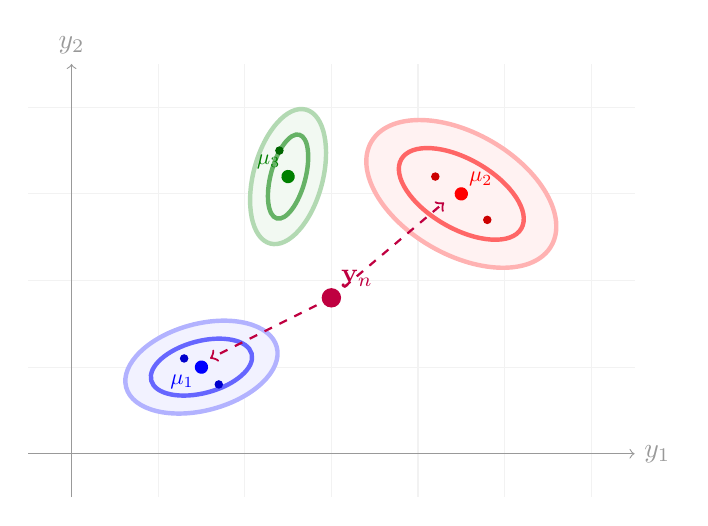
\begin{tikzpicture}[scale=1.1]
    % Draw background grid
    \draw[black!5, step=1] (-0.5,-0.5) grid (6.5,4.5);
    \draw[->, black!40] (-0.5,0) -- (6.5,0) node[right] {$y_1$};
    \draw[->, black!40] (0,-0.5) -- (0,4.5) node[above] {$y_2$};

    % Cluster 1 (Blue) - Bottom Left
    \begin{scope}[shift={(1.5,1)}, rotate=15]
        \draw[blue!30, fill=blue!5, ultra thick] (0,0) ellipse (0.9cm and 0.5cm);
        \draw[blue!60, ultra thick] (0,0) ellipse (0.6cm and 0.3cm);
        \filldraw[blue] (0,0) circle (2pt) node[below left, scale=0.8] {$\boldsymbol{\mu}_1$};
    \end{scope}
    \filldraw[blue!80!black] (1.3,1.1) circle (1.2pt);
    \filldraw[blue!80!black] (1.7,0.8) circle (1.2pt);

    % Cluster 2 (Red) - Top Right
    \begin{scope}[shift={(4.5,3)}, rotate=-30]
        \draw[red!30, fill=red!5, ultra thick] (0,0) ellipse (1.2cm and 0.7cm);
        \draw[red!60, ultra thick] (0,0) ellipse (0.8cm and 0.4cm);
        \filldraw[red] (0,0) circle (2pt) node[above right, scale=0.8] {$\boldsymbol{\mu}_2$};
    \end{scope}
    \filldraw[red!80!black] (4.2,3.2) circle (1.2pt);
    \filldraw[red!80!black] (4.8,2.7) circle (1.2pt);

    % Cluster 3 (Green) - Center Top
    \begin{scope}[shift={(2.5,3.2)}, rotate=75]
        \draw[green!50!black!30, fill=green!50!black!5, ultra thick] (0,0) ellipse (0.8cm and 0.4cm);
        \draw[green!50!black!60, ultra thick] (0,0) ellipse (0.5cm and 0.2cm);
        \filldraw[green!50!black] (0,0) circle (2pt) node[above left, scale=0.8] {$\boldsymbol{\mu}_3$};
    \end{scope}
    \filldraw[green!40!black] (2.4,3.5) circle (1.2pt);

    % Complex Ambiguous Query Point
    \filldraw[purple] (3.0,1.8) circle (3pt) node[above right] {$\mathbf{y}_n$};
    \draw[->, dashed, purple, thick] (3.0,1.8) -- (1.6,1.1);
    \draw[->, dashed, purple, thick] (3.0,1.8) -- (4.3,2.9);
\end{tikzpicture}
\caption{Visualizing a 2D GMM with $K=3$ separate Gaussian components. When an ambiguous data point $\mathbf{y}_n$ arrives in the dead-zone between clusters, the system uses Bayes' rule to calculate a soft fractional ownership profile.}
\label{fig:gmm_contours}
\end{figure}

GMMs are incredibly powerful because they act like mathematical clay. If you pack enough individual Gaussians into a single mixture model, you can approximate \textbf{any smooth, arbitrary probability density shape} in existence.

\subsection*{18.3. Responsibilities: Soft vs. Hard Clustering}
GMMs are widely used for \textbf{unsupervised clustering} (grouping data together without pre-existing labels). Once a GMM is optimized and fitted to a cloud of data points, we can use it to diagnose where any individual data point $\mathbf{y}_n$ originated.

We do this by calculating the posterior probability of the hidden variable $z_n$ using Bayes' rule. This specific calculation is known as the **Responsibility** ($r_{nk}$), which measures exactly how much cluster $k$ is "to blame" for creating data point $n$:
\begin{equation}
r_{nk} \triangleq p(z_n = k \mid \mathbf{y}_n, \boldsymbol{\theta}) = \frac{p(z_n = k \mid \boldsymbol{\theta}) p(\mathbf{y}_n \mid z_n = k, \boldsymbol{\theta})}{\sum_{k'=1}^K p(z_n = k' \mid \boldsymbol{\theta}) p(\mathbf{y}_n \mid z_n = k', \boldsymbol{\theta})} = \frac{\pi_k \mathcal{N}(\mathbf{y}_n \mid \boldsymbol{\mu}_k, \boldsymbol{\Sigma}_k)}{\sum_{k'=1}^K \pi_{k'} \mathcal{N}(\mathbf{y}_n \mid \boldsymbol{\mu}_{k'}, \boldsymbol{\Sigma}_{k'})} \tag{116}
\end{equation}

Depending on how you use these responsibilities, you can perform two different types of clustering:
\begin{itemize}
    \item \textbf{Soft Clustering:} You retain the full fractional percentages of $r_{nk}$. For instance, a boundary data point might be classified as $65\%$ belonging to Cluster 1 and $35\%$ belonging to Cluster 2. This accurately preserves uncertainty.
    \item \textbf{Hard Clustering:} You force the system to make a definitive choice. You assign the data point exclusively to the single cluster that achieves the absolute highest responsibility value:
    \begin{align}
    \hat{z}_n &= \arg\max_k r_{nk} \nonumber \\
    &= \arg\max_k \left[ \ln \mathcal{N}(\mathbf{y}_n \mid \boldsymbol{\mu}_k, \boldsymbol{\Sigma}_k) + \ln \pi_k \right] \tag{117}
    \end{align}
\end{itemize}

\subsection*{18.4. How GMM Collapses into standard K-Means}
There is a direct mathematical bridge between the probabilistic, smooth world of GMMs and the rigid, geometric world of the classic \textbf{K-means clustering algorithm}. 

If we take a standard GMM and strip away its flexibility by applying two extreme simplifying assumptions:
\begin{enumerate}
    \item \textbf{Uniform Weights:} Assume all clusters have an equal probability of being picked ($\pi_k = 1/K$).
    \item \textbf{Spherical Identity Noise:} Assume every cluster is a perfectly round circle with identical, microscopic variance ($\boldsymbol{\Sigma}_k = \sigma^2 \mathbf{I}$, where $\sigma^2 \to 0$).
\end{enumerate}

When you plug these restrictions into the hard-clustering equation (Equation 117), the log-likelihood of a Gaussian turns directly into a squared Euclidean distance penalty. The entire probabilistic calculation collapses down into:
\begin{equation}
\hat{z}_n = \arg\min_k ||\mathbf{y}_n - \hat{\boldsymbol{\mu}}_k||_2^2 \tag{118}
\end{equation}

This is the exact operational loop of the K-means algorithm! K-means is simply a stripped-down, rigid version of a GMM that drops all information about shape, orientation, and cluster size, choosing to assign data strictly based on raw distance to the closest center.

\section*{19. Bernoulli Mixture Models (BMMs)}

While Gaussian Mixture Models (GMMs) are perfect for continuous real-valued measurements (like heights, weights, or spatial coordinates), they break down completely when your data is strictly binary (zeros and ones, yes/no responses, or black-and-white pixels). 

A \textbf{Bernoulli Mixture Model (BMM)}, or a mixture of Bernoullis, is designed specifically for multi-dimensional binary data vectors. Instead of mixing continuous bell curves, a BMM blends together collections of independent coin flips.

\subsection*{19.1. The Mathematical Blueprint}
Imagine a dataset where each observation $\mathbf{y}$ is a $D$-dimensional vector of bits: $\mathbf{y} = [y_1, y_2, \dots, y_D]^T$, where $y_d \in \{0, 1\}$. 

If we assign this data point to a specific hidden cluster $k$, the probability of seeing this exact sequence of bits is modeled by multiplying $D$ independent Bernoulli trials together:
\begin{equation}
p(\mathbf{y} \mid z = k, \boldsymbol{\theta}) = \prod_{d=1}^D \text{Ber}(y_d \mid \mu_{dk}) = \prod_{d=1}^D \mu_{dk}^{y_d} (1 - \mu_{dk})^{1 - y_d} \tag{119}
\end{equation}

Where:
\begin{itemize}
    \item $z = k$ is the active hidden cluster identity.
    \item $\mu_{dk}$ is a probability value between $0$ and $1$ representing the "knob setting" for the $d$-th dimension inside cluster $k$. It answers the question: \textit{"What is the probability that bit $d$ will turn on (equal 1) if it belongs to cluster $k$?"}
\end{itemize}

\paragraph{The Paradox of Conditional Independence}
Look closely at Equation (119). We calculate the total probability by simply multiplying individual pixel probabilities together. This implies that within any single cluster, the dimensions are assumed to be \textbf{completely independent} of each other. 

At first glance, this sounds like a terrible assumption for images. If pixel $(x, y)$ is part of a handwritten line, the neighboring pixel $(x+1, y)$ is highly likely to be part of that line too—they are clearly dependent. 

However, the magic of mixture models is that when you sum these components together using mixing weights ($\pi_k$), the resulting global distribution is capable of capturing incredibly complex, non-linear correlations across dimensions:
\begin{equation}
p(\mathbf{y} \mid \boldsymbol{\theta}) = \sum_{k=1}^K \pi_k \left[ \prod_{d=1}^D \mu_{dk}^{y_d} (1 - \mu_{dk})^{1 - y_d} \right] \tag{120}
\end{equation}
By layering multiple simple, independent templates on top of each other, the model acts as a powerful global feature detector.

\subsection*{19.2. Structural Architecture of a BMM}
The diagram below shows how a single binary input data vector gets processed by separate cluster templates inside a BMM to calculate matching probabilities.

\begin{figure}[H]
\centering
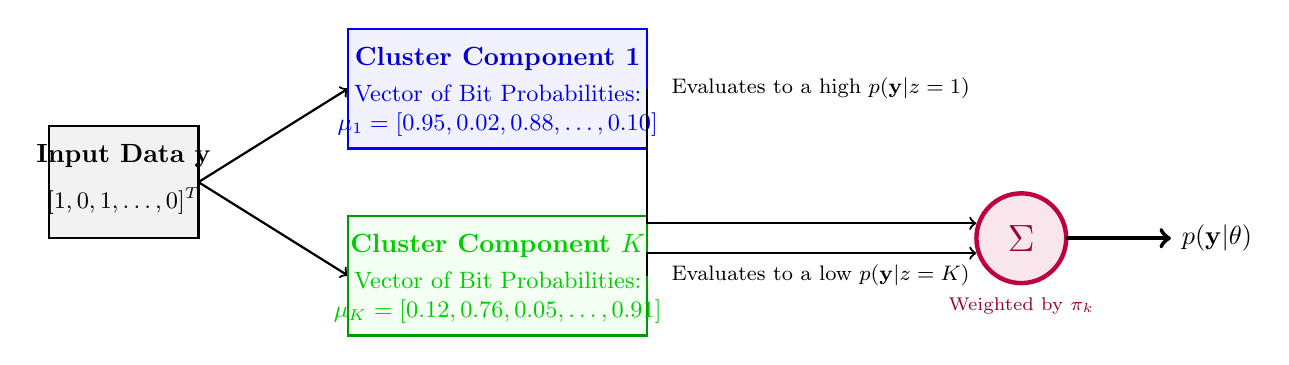
\begin{tikzpicture}[scale=0.95, every node/.style={transform shape}]
    % Input Vector Box
    \draw[black, thick, fill=gray!10] (-3, 1) rectangle (-1, 2.5);
    \node[font=\bfseries] at (-2, 2.1) {Input Data $\mathbf{y}$};
    \node[font=\small] at (-2, 1.5) {$[1, 0, 1, \dots, 0]^T$};
    
    % Arrows out to components
    \draw[->, thick] (-1, 1.75) -- (1, 3);
    \draw[->, thick] (-1, 1.75) -- (1, 0.5);

    % Cluster 1 Template Box
    \draw[blue, thick, fill=blue!5] (1, 2.2) rectangle (5, 3.8);
    \node[blue!80!black, font=\bfseries] at (3, 3.4) {Cluster Component 1};
    \node[blue!90!black, font=\small, align=center] at (3, 2.7) {Vector of Bit Probabilities: \\ $\boldsymbol{\mu}_1 = [0.95, 0.02, 0.88, \dots, 0.10]$};

    % Cluster K Template Box
    \draw[green!60!black, thick, fill=green!5] (1, -0.3) rectangle (5, 1.3);
    \node[green!80!black, font=\bfseries] at (3, 0.9) {Cluster Component $K$};
    \node[green!80!black, font=\small, align=center] at (3, 0.2) {Vector of Bit Probabilities: \\ $\boldsymbol{\mu}_K = [0.12, 0.76, 0.05, \dots, 0.91]$};

    % Evaluation Nodes
    \node[anchor=west, font=\footnotesize] at (5.2, 3) {Evaluates to a high $p(\mathbf{y}|z=1)$};
    \node[anchor=west, font=\footnotesize] at (5.2, 0.5) {Evaluates to a low $p(\mathbf{y}|z=K)$};

    % Summation Block
    \draw[purple, ultra thick, fill=purple!10] (10, 1) circle (0.6cm);
    \node[purple!80!black, font=\Large\bfseries] at (10, 1) {$\Sigma$};
    \node[purple!80!black, font=\scriptsize, align=center] at (10, 0.1) {Weighted by $\pi_k$};

    % Connect to sum
    \draw[->, thick] (5, 3) |- (9.4, 1.2);
    \draw[->, thick] (5, 0.5) |- (9.4, 0.8);
    
    % Output
    \draw[->, ultra thick] (10.6, 1) -- (12, 1) node[right, font=\bfseries] {$p(\mathbf{y}|\boldsymbol{\theta})$};
\end{tikzpicture}
\caption{Operational breakdown of a Bernoulli Mixture Model. The input binary vector is evaluated against each independent cluster template, and the results are combined into a single unified probability output via the mixing weights.}
\label{fig:bmm_architecture}
\end{figure}

\subsection*{19.3. Unsupervised Magic: The MNIST Digit Example}
To see why this is useful, look at how a BMM interacts with the famous MNIST dataset (a collection of thousands of $28 \times 28$ grayscale images of handwritten digits from $0$ to $9$). 

First, we binarize the data: any pixel that has ink becomes a $1$, and any empty background pixel becomes a $0$. This turns each image into a 784-dimensional binary vector ($D = 28 \times 28 = 784$).

Next, we throw away all human-provided labels. The model has absolutely no idea what a "3", a "7", or an "8" is. We configure a BMM with $K = 20$ hidden clusters and train it on these raw unlabelled binary vectors using an optimization algorithm (like Expectation-Maximization or Stochastic Gradient Descent). 

During training, the model performs automatic feature discovery:
\begin{itemize}
    \item \textbf{Statistical Convergence:} The 784 parameters ($\mu_{1k}, \mu_{2k}, \dots, \mu_{784,k}$) inside each cluster $k$ begin to shift. They coordinate to optimize the global likelihood of the data.
    \item \textbf{The Emergence of Templates:} If you take the final optimized $\boldsymbol{\mu}_k$ vector for a specific cluster and render those fractional probabilities back as a grayscale image, a clear, smooth, ghostly archetype of a specific handwritten number appears automatically. 
    \item \textbf{Handling Variations:} Because humans write numbers using different styles, the unsupervised model might dedicate 3 distinct clusters to the number "7" (e.g., one cluster for a straight 7, one for a slanted 7, and one for a 7 with a cross-bar). It does this purely because grouping them this way makes the data structurally more predictable.
\end{itemize}

By viewing the cluster centers, we can confirm that without a single human hint, the BMM automatically disentangles the chaotic soup of pixel combinations, categorizing them into distinct, human-interpretable structural concepts.

\subsection*{19.4. Worked Numerical Example: Gaussian Mixture Model (GMM)}

To see exactly how a Gaussian Mixture Model processes information under the hood, let's solve a 1D numerical problem step-by-step.

Imagine a machine learning model has already been trained to cluster data into $K=2$ hidden groups. The learned parameters for the two clusters are:
\begin{itemize}
    \item \textbf{Cluster 1 (Narrow bell curve):} Mixing weight $\pi_1 = 0.4$, Mean $\mu_1 = 2.0$, Variance $\sigma_1^2 = 1.0$ ($\sigma_1 = 1$)
    \item \textbf{Cluster 2 (Wide bell curve):} Mixing weight $\pi_2 = 0.6$, Mean $\mu_2 = 5.0$, Variance $\sigma_2^2 = 4.0$ ($\sigma_2 = 2$)
\end{itemize}

A new continuous data point arrives at coordinate \textbf{$y = 3.0$}. We want to determine the total probability of observing this data point and find out which cluster structurally "owns" it.

\paragraph{Step 1: Calculate Individual Component Probabilities}
First, we find out how likely our data point $y=3.0$ is under each individual Gaussian template using the classic normal distribution density formula:
\begin{equation*}
\mathcal{N}(y \mid \mu, \sigma^2) = \frac{1}{\sqrt{2\pi\sigma^2}} \exp\left( -\frac{(y - \mu)^2}{2\sigma^2} \right)
\end{equation*}

For \textbf{Cluster 1}:
\begin{align}
\mathcal{N}(3.0 \mid 2.0, 1.0) &= \frac{1}{\sqrt{2\pi(1)}} \exp\left( -\frac{(3 - 2)^2}{2(1)} \right) \nonumber \\
&= \frac{1}{\sqrt{2\pi}} \exp(-0.5) \approx 0.3989 \times 0.6065 = \mathbf{0.2420} \tag{121}
\end{align}

For \textbf{Cluster 2}:
\begin{align}
\mathcal{N}(3.0 \mid 5.0, 4.0) &= \frac{1}{\sqrt{2\pi(4)}} \exp\left( -\frac{(3 - 5)^2}{2(4)} \right) \nonumber \\
&= \frac{1}{2\sqrt{2\pi}} \exp\left(-\frac{4}{8}\right) = \frac{0.3989}{2} \exp(-0.5) \approx 0.1994 \times 0.6065 = \mathbf{0.1210} \tag{122}
\end{align}

\paragraph{Step 2: Compute Total Marginal Probability $p(y)$}
Using our mixture rule from Equation (115), we scale each individual density value by its respective mixing weight percentage ($\pi_k$) and sum them together:
\begin{align}
p(y=3.0 \mid \boldsymbol{\theta}) &= \pi_1 \mathcal{N}(3.0 \mid \mu_1, \sigma_1^2) + \pi_2 \mathcal{N}(3.0 \mid \mu_2, \sigma_2^2) \nonumber \\
&= 0.4(0.2420) + 0.6(0.1210) \nonumber \\
&= 0.0968 + 0.0726 = \mathbf{0.1694} \tag{123}
\end{align}
The overall probability of seeing a data point at $y=3.0$ across the entire combined ecosystem is $16.94\%$.

\paragraph{Step 3: Calculate Posterior Soft Responsibilities ($r_{nk}$)}
Now we apply Bayes' rule to discover which cluster is responsible for creating this point. We divide each cluster's weighted contribution by the total overall probability:

For \textbf{Cluster 1}:
\begin{equation}
r_{11} = \frac{\pi_1 \mathcal{N}(3.0 \mid \mu_1, \sigma_1^2)}{p(y=3.0)} = \frac{0.0968}{0.1694} \approx \mathbf{0.5714} \quad (57.14\%) \tag{124}
\end{equation}

For \textbf{Cluster 2}:
\begin{equation}
r_{12} = \frac{\pi_2 \mathcal{N}(3.0 \mid \mu_2, \sigma_2^2)}{p(y=3.0)} = \frac{0.0726}{0.1694} \approx \mathbf{0.4286} \quad (42.86\%) \tag{125}
\end{equation}

\paragraph{Analysis of Results}
Notice the beautiful nuance here. The data point $y=3.0$ sits at distance $1.0$ from the center of Cluster 1 ($\mu_1=2$), but it sits distance $2.0$ away from Cluster 2 ($\mu_2=5$). Geometrically, it is physically closer to Cluster 1. 

However, because Cluster 2 has a much larger base mixing weight ($\pi_2 = 0.6$ vs $\pi_1 = 0.4$), it exerts a stronger baseline gravitational pull over the system. As a result, the soft clustering profile retains significant spatial ambiguity: the point has a $57.14\%$ chance of belonging to Cluster 1 and a $42.86\%$ chance of belonging to Cluster 2. 
If we were forced to make a \textbf{hard clustering} choice, we would assign it to Cluster 1 since $\hat{z} = \arg\max_k r_{1k} = 1$.


\subsection*{19.5. Worked Numerical Example: Bernoulli Mixture Model (BMM)}

Let's now work through a multi-dimensional binary problem to see how collections of coin flips collaborate.

Suppose you have a tiny binary image containing a vector of $D=3$ pixels. We have trained a model with $K=2$ hidden shape templates:
\begin{itemize}
    \item \textbf{Cluster 1 (Horizontal line pattern archetype):} Mixing weight $\pi_1 = 0.7$. \\ Pixel activation probabilities: $\boldsymbol{\mu}_1 = [\mu_{11}, \mu_{21}, \mu_{31}]^T = [0.9, 0.1, 0.8]^T$
    \item \textbf{Cluster 2 (Vertical line pattern archetype):} Mixing weight $\pi_2 = 0.3$. \\ Pixel activation probabilities: $\boldsymbol{\mu}_2 = [\mu_{12}, \mu_{22}, \mu_{32}]^T = [0.2, 0.8, 0.3]^T$
\end{itemize}

A new black-and-white sample vector arrives: $\mathbf{y} = [1, 0, 1]^T$ (meaning Pixel 1 is ON, Pixel 2 is OFF, Pixel 3 is ON). Let's evaluate this sample.

\paragraph{Step 1: Calculate Class-Conditional Probabilities}
We evaluate the product of the independent Bernoulli states for each cluster layout using Equation (119):

For \textbf{Cluster 1}:
\begin{align}
p(\mathbf{y} \mid z=1) &= \left[\mu_{11}^1 (1-\mu_{11})^0\right] \times \left[\mu_{21}^0 (1-\mu_{21})^1\right] \times \left[\mu_{31}^1 (1-\mu_{31})^0\right] \nonumber \\
&= (0.9) \times (1 - 0.1) \times (0.8) \nonumber \\
&= 0.9 \times 0.9 \times 0.8 = \mathbf{0.648} \tag{126}
\end{align}

For \textbf{Cluster 2}:
\begin{align}
p(\mathbf{y} \mid z=2) &= \left[\mu_{12}^1 (1-\mu_{12})^0\right] \times \left[\mu_{22}^0 (1-\mu_{22})^1\right] \times \left[\mu_{32}^1 (1-\mu_{32})^0\right] \nonumber \\
&= (0.2) \times (1 - 0.8) \times (0.3) \nonumber \\
&= 0.2 \times 0.2 \times 0.3 = \mathbf{0.012} \tag{127}
\end{align}

\paragraph{Step 2: Compute Total Marginal Probability $p(\mathbf{y})$}
We blend the conditional scores together using the mixing percentages:
\begin{align}
p(\mathbf{y} \mid \boldsymbol{\theta}) &= \pi_1 p(\mathbf{y} \mid z=1) + \pi_2 p(\mathbf{y} \mid z=2) \nonumber \\
&= 0.7(0.648) + 0.3(0.012) \nonumber \\
&= 0.4536 + 0.0036 = \mathbf{0.4572} \tag{128}
\end{align}

\paragraph{Step 3: Compute Responsibilities ($r_{nk}$)}
Finally, we calculate the posterior responsibility to see which template matches our data point's structural characteristics:

For \textbf{Cluster 1}:
\begin{equation}
r_{11} = \frac{\pi_1 p(\mathbf{y} \mid z=1)}{p(\mathbf{y})} = \frac{0.4536}{0.4572} \approx \mathbf{0.9921} \quad (99.21\%) \tag{129}
\end{equation}

For \textbf{Cluster 2}:
\begin{equation}
r_{12} = \frac{\pi_2 p(\mathbf{y} \mid z=2)}{p(\mathbf{y})} = \frac{0.0036}{0.4572} \approx \mathbf{0.0079} \quad (0.79\%) \tag{130}
\end{equation}

\paragraph{Analysis of Results}
The evaluation shows an overwhelming classification layout. Cluster 1 expected pixels 1 and 3 to be active while pixel 2 remained dark ($[0.9, 0.1, 0.8]^T$), which aligns perfectly with our observed vector $[1, 0, 1]^T$. 

Conversely, Cluster 2 wanted the exact opposite layout—it expected pixel 2 to be active while pixels 1 and 3 remained dark ($[0.2, 0.8, 0.3]^T$). Because our vector violated all three expectations of Cluster 2, its component probability dropped to a near-zero value ($0.012$). 

When combined with the higher baseline weight of Cluster 1 ($\pi_1 = 0.7$), Bayes' rule filters out almost all uncertainty. The model concludes with over $99.2\%$ confidence that this pixel sample belongs to Cluster 1.

\section*{20. Probabilistic Graphical Models (PGMs)}

If you try to model a complex real-world system with dozens of variables using a standard joint probability table, you will immediately hit an exponential wall. For example, a system with just 30 binary variables requires a table with $2^{30}$ rows (over a billion parameters!). It is computationally impossible to store, let alone train.

A \textbf{Probabilistic Graphical Model (PGM)} is a master optimization framework that solves this by combining \textbf{Graph Theory} with \textbf{Probability Theory}. It allows us to map out variables as visual nodes and use the presence or absence of connecting lines to slice a massive, unmanageable distribution into clean, modular, independent chunks.

\subsection*{20.1. The Core Architecture: Directed Acyclic Graphs (DAGs)}
When a PGM uses directed arrows without any closed feedback loops, it is called a \textbf{Bayesian Network} (or a Directed Acyclic Graph / DAG). 

The visual layout of the graph operates under a strict geometric law:
\begin{itemize}
    \item \textbf{Nodes} represent your random variables.
    \item \textbf{Edges (Arrows)} represent direct dependencies (causal paths or directional influences).
    \item \textbf{The Absence of an Arrow} is the structural superpower of a PGM. It explicitly states that two variables are \textbf{conditionally independent}.
\end{itemize}

\paragraph{The Factorization Fundamental Theorem}
Instead of dealing with a massive global joint table, a DAG mathematically guarantees that you can calculate the complete joint probability of any complex system by simply looking at each node individually and multiplying it by the probability of its immediate \textbf{parents}:
\begin{equation}
p(Y_1, Y_2, \dots, Y_{N_G}) = \prod_{i=1}^{N_G} p(Y_i \mid Y_{\text{pa}(i)}) \tag{131}
\end{equation}
Where $Y_{\text{pa}(i)}$ represents the direct parent nodes pointing into node $i$. This is called the \textbf{ordered Markov property}, and it cuts down the number of parameters needed from an exponential nightmare to a simple linear scale.

\subsection*{20.2. Visualizing the Water Sprinkler Network}
Let's look at the classic 4-variable textbook problem:
\begin{itemize}
    \item $C$: Whether it is a cloudy season ($T/F$).
    \item $R$: Whether it is raining ($T/F$).
    \item $S$: Whether your automatic lawn sprinkler is turned on ($T/F$).
    \item $W$: Whether the grass is wet ($T/F$).
\end{itemize}

Without a graph, the raw chain rule of probability forces us to write a bloated joint equation:
\begin{equation*}
p(C, S, R, W) = p(C) \cdot p(S \mid C) \cdot p(R \mid C, S) \cdot p(W \mid C, S, R)
\end{equation*}

Now let's apply real-world structural knowledge to create a clean visual dependency map using a colored TikZ network diagram:

\begin{figure}[H]
\centering
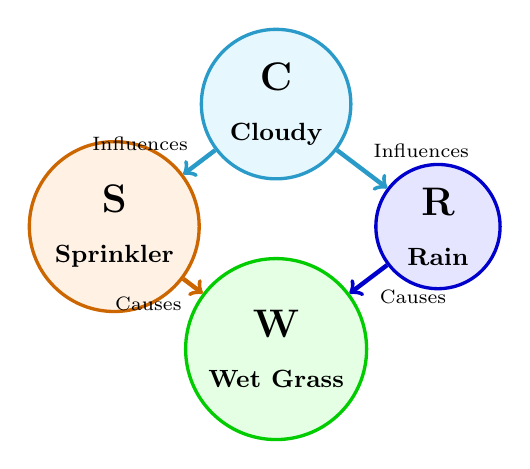
\begin{tikzpicture}[
    node distance=2.2cm,
    roundnode/.style={circle, draw=black!80, fill=gray!8, very thick, minimum size=1.2cm, font=\bfseries\Large, align=center}
]
    % Nodes
    \node[roundnode, fill=cyan!10, draw=cyan!80!black] (C) {C \\ \small Cloudy};
    \node[roundnode, fill=orange!10, draw=orange!80!black, below left of=C, xshift=-0.5cm] (S) {S \\ \small Sprinkler};
    \node[roundnode, fill=blue!10, draw=blue!80!black, below right of=C, xshift=0.5cm] (R) {R \\ \small Rain};
    \node[roundnode, fill=green!10, draw=green!80!black, below right of=S, xshift=0.5cm] (W) {W \\ \small Wet Grass};

    % Edges with labels
    \draw[->, ultra thick, cyan!80!black] (C) -- node[above left, font=\scriptsize, black] {Influences} (S);
    \draw[->, ultra thick, cyan!80!black] (C) -- node[above right, font=\scriptsize, black] {Influences} (R);
    \draw[->, ultra thick, orange!80!black] (S) -- node[below left, font=\scriptsize, black] {Causes} (W);
    \draw[->, ultra thick, blue!80!black] (R) -- node[below right, font=\scriptsize, black] {Causes} (W);
    
\end{tikzpicture}
\caption{The visual architecture of the classic 4-node Water Sprinkler DAG network.}
\label{fig:sprinkler_dag}
\end{figure}

Look closely at the layout of Figure \ref{fig:sprinkler_dag} to see how conditional independence strips down our joint probability equation:
\begin{enumerate}
    \item \textbf{Isolating Rain ($R$):} In the full chain rule, we had $p(R \mid C, S)$. But looking at our graph, the sprinkler ($S$) has no arrow connecting to rain ($R$). Once we know if it is cloudy ($C$), the state of the sprinkler gives us zero extra information about rain. Thus, $p(R \mid C, S) \to p(R \mid C)$.
    \item \textbf{Isolating Wet Grass ($W$):} In the full chain rule, we had $p(W \mid C, S, R)$. But looking at our graph, the cloudy node ($C$) has no direct path to wet grass except through $S$ and $R$. If we already know for a fact that it is raining and the sprinkler is running, knowing whether it is cloudy adds absolutely nothing to our prediction of the grass being wet. Thus, $p(W \mid C, S, R) \to p(W \mid S, R)$.
\end{enumerate}

By dropping these redundant context connections, our master joint factorization collapses down into a beautifully lean, modular product form:
\begin{equation}
p(C, S, R, W) = p(C) \cdot p(S \mid C) \cdot p(R \mid C) \cdot p(W \mid S, R) \tag{132}
\end{equation}

\subsection*{20.3. Conditional Probability Tables (CPTs)}
For discrete networks, each node contains a local \textbf{Conditional Probability Table (CPT)}. Each row of a CPT represents a unique combination of values for that node's parents, and the values across any single row must sum to exactly $1.0$.

Let's write down the exact numeric parameters ($\theta_{ijk}$) for our Water Sprinkler network based on the textbook configurations:

\begin{table}[H]
\centering
\small
\begin{tabular}{|c|cc|}
\hline
\multicolumn{3}{|c|}{\textbf{Node C: Cloudy}} \\ \hline
& \textbf{P(C=False)} & \textbf{P(C=True)} \\ \cline{2-3} 
& 0.5 & 0.5 \\ \hline
\end{tabular}
\quad
\begin{tabular}{|c|cc|}
\hline
\multicolumn{3}{|c|}{\textbf{Node S: Sprinkler}} \\ \hline
\textbf{Parent C} & \textbf{P(S=False)} & \textbf{P(S=True)} \\ \hline
\textbf{False} & 0.5 & 0.5 \\
\textbf{True} & 0.9 & 0.1 \\ \hline
\end{tabular}
\vspace{0.3cm}

\begin{tabular}{|c|cc|}
\hline
\multicolumn{3}{|c|}{\textbf{Node R: Rain}} \\ \hline
\textbf{Parent C} & \textbf{P(R=False)} & \textbf{P(R=True)} \\ \hline
\textbf{False} & 0.8 & 0.2 \\
\textbf{True} & 0.2 & 0.8 \\ \hline
\end{tabular}
\quad
\begin{tabular}{|cc|cc|}
\hline
\multicolumn{4}{|c|}{\textbf{Node W: Wet Grass}} \\ \hline
\textbf{Parent S} & \textbf{Parent R} & \textbf{P(W=False)} & \textbf{P(W=True)} \\ \hline
\textbf{False} & \textbf{False} & 1.0 & 0.0 \\
\textbf{True} & \textbf{False} & 0.1 & 0.9 \\
\textbf{False} & \textbf{True} & 0.1 & 0.9 \\
\textbf{True} & \textbf{True} & 0.01 & 0.99 \\ \hline
\end{tabular}
\caption{The local structural CPT parameters governing our network system.}
\label{tab:cpts}
\end{table}

Notice how much data compression occurred here. A raw 4-variable joint table requires $2^4 - 1 = 15$ independent parameters to track. By factoring the network into small local tables, we only need to store $1 + 2 + 2 + 4 = 9$ parameters. This parameter gap grows rapidly as systems become larger!

\subsection*{20.4. Fully Worked Numerical Inference Example}

Let's compute an exact joint query using our modular CPT tables.

\paragraph{Problem Scenario}
Calculate the exact probability of encountering a specific day where:
\begin{itemize}
    \item It is \textbf{Cloudy} ($C = \text{True}$)
    \item The \textbf{Sprinkler} is OFF** ($S = \text{False}$)
    \item It is \textbf{Raining} ($R = \text{True}$)
    \item The \textbf{Grass is WET} ($W = \text{True}$)
\end{itemize}
Mathematically, we are looking for the joint calculation value: $p(C=T, S=F, R=T, W=T)$.

\paragraph{Step-by-Step Calculation Loop}
We pull our factorized equation layout from Equation (132) and substitute our target variable values directly into it:
\begin{equation}
p(C=T, S=F, R=T, W=T) = p(C=T) \cdot p(S=F \mid C=T) \cdot p(R=T \mid C=T) \cdot p(W=T \mid S=F, R=T) \tag{133}
\end{equation}

Now, let's look up each individual value from our CPT tables in Table \ref{tab:cpts}:
\begin{itemize}
    \item Baseline prior for cloudy season: $\quad p(C=T) = \mathbf{0.5}$
    \item Probability sprinkler is off given it's cloudy: $\quad p(S=F \mid C=T) = \mathbf{0.9}$
    \item Probability it rains given it's cloudy: $\quad p(R=T \mid C=T) = \mathbf{0.8}$
    \item Probability grass is wet given no sprinkler but active rain: $\quad p(W=T \mid S=F, R=T) = \mathbf{0.9}$
\end{itemize}

Plugging these parameters back into our product chain yields:
\begin{align}
p(C=T, S=F, R=T, W=T) &= (0.5) \times (0.9) \times (0.8) \times (0.9) \nonumber \\
&= 0.45 \times 0.8 \times 0.9 \nonumber \\
&= 0.36 \times 0.9 \nonumber \\
&= \mathbf{0.324} \tag{134}
\end{align}

\paragraph{Conclusion}
There is an exact \textbf{32.4\%} chance of encountering this specific world state configuration. 

Look at how straightforward that was. We did not have to search through a massive 16-row global database table. By mapping the system's conditional independence dependencies as a graphical flowchart, we broke a multi-variable joint problem down into a series of simple lookups across isolated local tables. This structural modularity forms the backbone of modern large-scale statistical AI systems.

\section*{21. Markov Chains and Sequential Language Modeling}

When dealing with sequential data—such as words in a sentence, stock prices over time, or genetic codes in a DNA strand—the order of variables changes everything. The meaning of a word depends heavily on what was said before it. 

If we try to model a sequence of $T$ variables ($y_1, y_2, \dots, y_T$) using the standard raw chain rule of probability, the mathematical expression expands into a historical dependency nightmare:
\begin{equation}
p(y_1, y_2, \dots, y_T) = p(y_1) \cdot p(y_2 \mid y_1) \cdot p(y_3 \mid y_1, y_2) \dots = \prod_{t=1}^T p(y_t \mid y_{1:t-1}) \tag{135}
\end{equation}

If our vocabulary has $K$ possible words, then predicting the 10th word requires calculating probabilities across a history of $K^9$ possible combinations. The model's parameter footprint grows \textbf{exponentially} with time, causing it to quickly collapse under its own weight.

A \textbf{Markov Chain} provides a clean, memory-efficient way out. It operates on a simple, elegant assumption about time: \textit{To predict the future, you do not need to look at the entire past. You only need to look at the immediate present.}

\subsection*{21.1. First-Order Markov Chains (The Bigram Model)}
The \textbf{First-Order Markov Assumption} mathematically declares that the future state $y_{t+1}$ is conditionally independent of all historical past states ($y_1, \dots, y_{t-1}$) once you know the current state $y_t$:
\begin{equation}
y_{t+1} \perp y_{1:t-1} \mid y_t \tag{136}
\end{equation}

When you apply this structural constraint to the chain rule factorization (Equation 135), the historical context drops away. The massive joint sequence probability collapses down into a highly efficient product of step-by-step state links:
\begin{equation}
p(y_1, y_2, \dots, y_T) = p(y_1) \cdot p(y_2 \mid y_1) \cdot p(y_3 \mid y_2) \cdot p(y_4 \mid y_3) \dots = p(y_1) \prod_{t=2}^T p(y_t \mid y_{t-1}) \tag{137}
\end{equation}
In computational linguistics, this is known as a \textbf{Bigram Language Model} because it treats a sentence as a connected chain of two-word pairs.

\paragraph{The Magic of Stationary Transition Matrices}
The conditional distribution $p(y_t \mid y_{t-1})$ is called the \textbf{Transition Kernel} or \textbf{Transition Function}. It tells us the probability of jumping from a specific state yesterday to a new state today.

If we assume that these transition probabilities remain constant over time, the sequence is called \textbf{homogeneous} or \textbf{time-invariant}. This introduces a powerful machine learning concept known as \textbf{parameter tying}: the exact same transition rules are reused across every single time step. This lets us model an infinitely long sequence using a completely fixed, finite number of parameters.

We can organize these fixed probabilities into a square $K \times K$ table called a \textbf{Stochastic Transition Matrix} ($\mathbf{A}$):
\begin{equation}
A_{jk} \triangleq p(y_t = k \mid y_{t-1} = j) \tag{138}
\end{equation}
Where every value is bounded between 0 and 1, and every row sums to exactly $1.0$ (since you must transition *somewhere* on the next step): $\sum_{k=1}^K A_{jk} = 1$.

\subsection*{21.2. Visual Architecture of Sequence Models}
Let's visually compare how information flows through a 1st-order Markov chain versus a more complex 2nd-order chain using a colored TikZ graphical network template.

\begin{figure}[H]
\centering
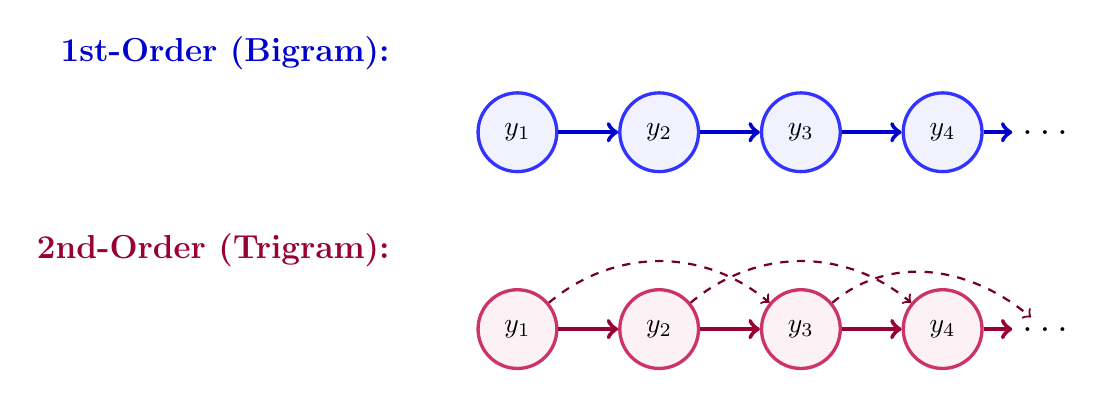
\begin{tikzpicture}[
    node distance=1.8cm,
    chainnode/.style={circle, draw=blue!80, fill=blue!5, very thick, minimum size=1.0cm, font=\bfseries}
]
    % --- FIRST ORDER CHAINS ---
    \node at (-1.5, 1) [left, font=\bfseries\large, color=blue!80!black] {1st-Order (Bigram):};
    \node[chainnode] (y1) {$y_1$};
    \node[chainnode, right of=y1] (y2) {$y_2$};
    \node[chainnode, right of=y2] (y3) {$y_3$};
    \node[chainnode, right of=y3] (y4) {$y_4$};
    \node[right of=y4, xshift=-0.5cm, font=\bfseries\Large] (ydot) {$\dots$};

    \draw[->, ultra thick, blue!80!black] (y1) -- (y2);
    \draw[->, ultra thick, blue!80!black] (y2) -- (y3);
    \draw[->, ultra thick, blue!80!black] (y3) -- (y4);
    \draw[->, ultra thick, blue!80!black] (y4) -- (ydot);

    % --- SECOND ORDER CHAINS ---
    \begin{scope}[yshift=-2.5cm, chainnode/.style={circle, draw=purple!80, fill=purple!5, very thick, minimum size=1.0cm, font=\bfseries}]
        \node at (-1.5, 1) [left, font=\bfseries\large, color=purple!80!black] {2nd-Order (Trigram):};
        \node[chainnode] (z1) {$y_1$};
        \node[chainnode, right of=z1] (z2) {$y_2$};
        \node[chainnode, right of=z2] (z3) {$y_3$};
        \node[chainnode, right of=z3] (z4) {$y_4$};
        \node[right of=z4, xshift=-0.5cm, font=\bfseries\Large] (zdot) {$\dots$};

        % Direct sequential connections
        \draw[->, ultra thick, purple!80!black] (z1) -- (z2);
        \draw[->, ultra thick, purple!80!black] (z2) -- (z3);
        \draw[->, ultra thick, purple!80!black] (z3) -- (z4);
        \draw[->, ultra thick, purple!80!black] (z4) -- (zdot);
        
        % Skip historical connections
        \draw[->, thick, dashed, purple!60!black] (z1) to[out=40, in=140] (z3);
        \draw[->, thick, dashed, purple!60!black] (z2) to[out=40, in=140] (z4);
        \draw[->, thick, dashed, purple!60!black] (z3) to[out=40, in=140] (zdot);
    \end{scope}
\end{tikzpicture}
\caption{Comparing information dependency structures. Top: A 1st-order chain where state $y_t$ depends solely on $y_{t-1}$. Bottom: A 2nd-order chain (Trigram Model) where state $y_t$ maintains a short historical window, looking back at both $y_{t-1}$ and $y_{t-2}$.}
\label{fig:markov_orders}
\end{figure}

\subsection*{21.3. Extending Memory: $M$-th Order Markov Chains}
While a first-order model is highly efficient, it has short-term amnesia. If a language model only looks at the single current word, it cannot maintain structural context over longer phrases. 

To improve this, we can extend the memory window to look back across $M$ historical states, creating an \textbf{$M$-th Order Markov Model}:
\begin{equation}
p(y_1, y_2, \dots, y_T) = p(y_{1:M}) \prod_{t=M+1}^T p(y_t \mid y_{t-M:t-1}) \tag{139}
\end{equation}

For instance, when $M=2$, the current word $y_t$ depends directly on the previous two words ($y_{t-1}$ and $y_{t-2}$), as illustrated in the bottom section of Figure \ref{fig:markov_orders}. This is called a \textbf{Trigram Model}. 

\subsection*{21.4. Fully Worked Sequential Numerical Example}

Let's look at a concrete numerical example to see how a text sequence is evaluated.

Imagine a vocabulary of $K=3$ words: $\mathcal{V} = \{\text{"The"}, \text{"Cat"}, \text{"Sat"}\}$. Let's assign numerical state tracking values to these words:
\begin{equation*}
\text{"The"} \to \text{State 1}, \quad \text{"Cat"} \to \text{State 2}, \quad \text{"Sat"} \to \text{State 3}
\end{equation*}

We have a 1st-order stationary Markov model governed by an initial starting probability vector $\boldsymbol{\pi}$ and a state transition matrix $\mathbf{A}$:
\begin{equation*}
\boldsymbol{\pi} = \begin{bmatrix} p(y_1=1) \\ p(y_1=2) \\ p(y_1=3) \end{bmatrix} = \begin{bmatrix} 0.8 \\ 0.1 \\ 0.1 \end{bmatrix}, \quad 
\mathbf{A} = \begin{bmatrix} 
0.1 & 0.7 & 0.2 \\ 
0.1 & 0.1 & 0.8 \\ 
0.4 & 0.3 & 0.3 
\end{bmatrix}
\end{equation*}

Let's decipher what row 2 of matrix $\mathbf{A}$ is telling us: if the current word at time $t-1$ is State 2 ("Cat"), then on the next step $t$, there is a $10\%$ chance of repeating "The", a $10\%$ chance of repeating "Cat", and an $80\%$ chance of transitioning to State 3 ("Sat").

\paragraph{Problem Scenario}
Calculate the exact joint probability of generating the 3-word sequence: \textbf{"The Cat Sat"}. \\
This corresponds to evaluating: $p(y_1=1, y_2=2, y_3=3)$.

\paragraph{Step-by-Step Calculation Loop}
Using our 1st-order Markov factorization rule from Equation (137), we break the sentence joint score down into isolated individual link steps:
\begin{equation}
p(y_1=1, y_2=2, y_3=3) = p(y_1=1) \cdot p(y_2=2 \mid y_1=1) \cdot p(y_3=3 \mid y_2=2) \tag{140}
\end{equation}

Now, we perform lookups across our matrix coordinates:
\begin{itemize}
    \item \textbf{Initial Start:} Probability that the sentence begins with "The" ($y_1=1$):
    \begin{equation*}
    p(y_1=1) = \pi_1 = \mathbf{0.8}
    \end{equation*}
    \item \textbf{First Transition:} Probability of jumping from "The" ($y_1=1$) to "Cat" ($y_2=2$):
    \begin{equation*}
    p(y_2=2 \mid y_1=1) = A_{12} = \mathbf{0.7}
    \end{equation*}
    \item \textbf{Second Transition:} Probability of jumping from "Cat" ($y_2=2$) to "Sat" ($y_3=3$):
    \begin{equation*}
    p(y_3=3 \mid y_2=2) = A_{23} = \mathbf{0.8}
    \end{equation*}
\end{itemize}

We multiply these local values together to find the final sequential probability:
\begin{align}
p(\text{"The Cat Sat"}) &= 0.8 \times 0.7 \times 0.8 \nonumber \\
&= 0.56 \times 0.8 \nonumber \\
&= \mathbf{0.448} \tag{141}
\end{align}

\paragraph{Conclusion}
Our Markov language model shows an exact \textbf{44.8\%} probability of generating this phrase.

\paragraph{Beyond N-Grams}
Notice that as $M$ grows larger to capture longer dependencies, our transition matrix expands rapidly, becoming a multi-dimensional tensor with $K^M$ cells. For real-world vocabularies with over $50,000$ words, $M$-gram models quickly become impossible to track. 

To overcome this, modern systems drop the discrete matrix table lookup approach and instead pass the historical token identities into neural networks to compute continuous predictions. This is the foundation of \textbf{Neural Language Models} and modern Transformers.

\section*{22. PGM Inference: The Explaining Away Effect}

Once a Probabilistic Graphical Model (PGM) maps out a complex system's conditional independence assumptions, we can use it to perform \textbf{inference}. Graphical inference is simply the act of asking the model structural questions: given that we have observed a specific set of evidence variables $\mathbf{Y}_j = \mathbf{y}_j$, what is the updated posterior probability of our target query variables $\mathbf{Y}_i$? 

To calculate this, the model combines the core rules of probability: \textbf{conditioning} (restricting our view only to scenarios matching the evidence) and \textbf{marginalization} (summing out all other unrelated background variables).

\subsection*{22.1. Berkson's Paradox: A Courtroom Drama in the Grass}
To understand how information paths open and close dynamically inside a network during inference, we look at a phenomenon known as the \textbf{explaining away effect} (or Berkson's paradox).

Let's revisit the classic Water Sprinkler network from Figure 3.14. Suppose we are tracking two completely separate, independent causes that can make the grass wet: Rain ($R$) and our automatic lawn Sprinkler ($S$). Under a normal cloudy sky ($C$), these two events have no direct connection to each other—knowing the sprinkler is running tells you nothing about whether water is falling from the clouds. They are marginally independent.

Now, look at how our mathematical beliefs shift step-by-step as evidence accumulates:

\paragraph{Scenario 1: The Baseline Prior}
Before we look outside, our long-term baseline probability that it has rained on any given day is a coin flip:
\begin{equation}
p(R = \text{True}) = 0.5000 \quad (50.00\%) \tag{142}
\end{equation}

\paragraph{Scenario 2: Observing the Effect (Diagnostic Reasoning)}
You step outside and notice something: the lawn grass is completely wet ($W = \text{True}$). Because rain is a primary cause of wet grass, your internal belief that it rained immediately shoots up:
\begin{equation}
p(R = \text{True} \mid W = \text{True}) = 0.7079 \quad (70.79\%) \tag{143}
\end{equation}
The wet grass acts as a strong piece of circumstantial evidence pointing to rain.

\paragraph{Scenario 3: Introducing the Alternative Cause (Explaining Away)}
Now for the twist. You walk over to the side of the house and discover that the automatic water sprinkler is spinning and turned on ($S = \text{True}$). 

Watch what happens to your belief about the rain:
\begin{equation}
p(R = \text{True} \mid W = \text{True}, S = \text{True}) = 0.3204 \quad (32.04\%) \tag{144}
\end{equation}

Your confidence that it rained plummeted from $70.79\%$ all the way down to $32.04\%$—a score even lower than your baseline starting prior! 

\paragraph{Why does this happen?} 
The moment you discovered that the sprinkler was active, you uncovered a perfectly valid alternative explanation for the wet grass. The sprinkler \textbf{"explains away"} the evidence. While it is still entirely possible that it rained and the sprinkler ran at the same time, the logical necessity for rain to be the culprit has been dramatically reduced. 

This reveals a profound property of PGMs: \textbf{Conditional independence is dynamic.} Two variables that are completely independent can suddenly become highly dependent once you observe their shared child node.


\section*{23. Parameter Learning and the Generative Story}

What happens if we don't know the exact probabilities inside our local CPT tables? In the world of PGMs, we don't treat model training as a separate, distinct process. Instead, we treat unknown parameters ($\theta$) as \textbf{latent random variables} and add them directly into our visual graph network as hollow nodes.

This framework allows us to express a clear \textbf{generative story}—a step-by-step recipe explaining how nature collaborates with hidden parameters to print out our observed dataset $\mathcal{D} = (y_1, y_2, \dots, y_N)$.

\begin{enumerate}
    \item \textbf{Draw the Parameters:} Nature chooses a permanent global parameter setting $\theta$ from an initial prior distribution: $\theta \sim p(\theta)$.
    \item \textbf{Draw the Data Points:} Given that specific fixed parameter $\theta$, nature runs $N$ independent, identical trials to stamp out individual data values: $y_n \sim p(y \mid \theta)$.
\end{enumerate}

Because all data points are generated using the exact same $\theta$ knob setting, they are conditionally independent of one another given $\theta$. Mathematically, this allows us to factorize the global joint distribution of data and parameters into a clean product:
\begin{equation}
p(\mathcal{D}, \theta) = p(\theta) p(\mathcal{D} \mid \theta) = p(\theta) \prod_{n=1}^N p(y_n \mid \theta) \tag{145}
\end{equation}

Because the ordering of individual samples inside the product loop does not alter the final combined probability score, the dataset is said to be \textbf{exchangeable}.


\section*{24. Plate Notation: Cleaning Up Visual Clutter}

If we attempted to draw out every single data point node ($y_1, y_2, \dots, y_N$) for a dataset containing a million rows, our visual graph layout would stretch across miles of paper. To prevent this visual clutter, graphical models use a clean notation format known as a \textbf{plate}.

A plate is a visual bounding box drawn around a repeating variable node structure. It acts like a programming \textbf{\texttt{for-loop}}, compactly condensing a massive, unrolled sequence of identical independent nodes down into a single representative element.

\subsection*{24.1. Visual Representation of Plate Conversion}
The diagram below illustrates the exact architectural equivalence between an explicitly unrolled parameter-to-data layout and its clean, condensed plate notation counterpart.

\begin{figure}[H]
\centering
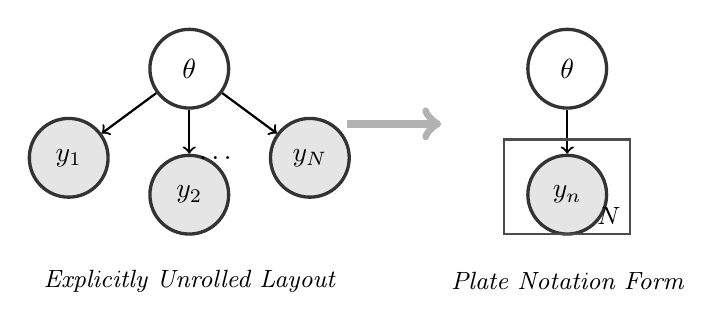
\begin{tikzpicture}[
    node distance=1.6cm,
    latent/.style={circle, draw=black!80, fill=white, very thick, minimum size=1.0cm, font=\bfseries},
    observed/.style={circle, draw=black!80, fill=gray!20, very thick, minimum size=1.0cm, font=\bfseries}
]
    % --- LEFT: UNROLLED ARCHITECTURE ---
    \node[latent] (theta1) {$\theta$};
    \node[observed, below left of=theta1, xshift=-0.4cm] (y1) {$y_1$};
    \node[observed, below of=theta1] (y2) {$y_2$};
    \node[observed, below right of=theta1, xshift=0.4cm] (yN) {$y_N$};
    \node[left of=yN, xshift=0.4cm, font=\bfseries] (ydots) {$\dots$};

    \draw[->, thick] (theta1) -- (y1);
    \draw[->, thick] (theta1) -- (y2);
    \draw[->, thick] (theta1) -- (yN);
    \node[below of=y2, yshift=0.5cm, font=\small\itshape] {Explicitly Unrolled Layout};

    % --- BRIDGE ARROW ---
    \draw[->, line width=3pt, gray!60] (2.0, -0.7) -- (3.2, -0.7);

    % --- RIGHT: COMPACT PLATE ARCHITECTURE ---
    \begin{scope}[xshift=4.8cm]
        \node[latent] (theta2) {$\theta$};
        \node[observed, below of=theta2] (yn) {$y_n$};
        \draw[->, thick] (theta2) -- (yn);

        % The Plate Box boundary (Enclosing just the data node)
        \draw[thick, draw=black!70, fill=none] (-0.8, -2.1) rectangle (0.8, -0.9);
        % Counter index label in the corner
        \node[anchor=south east, font=\small\bfseries] at (0.8, -2.1) {$N$};
        \node[below of=yn, yshift=0.5cm, font=\small\itshape] {Plate Notation Form};
    \end{scope}
\end{tikzpicture}
\caption{Collapsing an $N$-node sequence down into a single parameterized plate boundary container.}
\label{fig:plate_comparison}
\end{figure}

In Figure \ref{fig:plate_comparison}, the shaded color convention indicates an \textbf{observed node} (data we actually measured from the real world), while a hollow white node represents a \textbf{latent node} (hidden states, parameters, or cluster identities that we must uncover via inference).

\subsection*{24.2. Advanced Example: Dissecting a GMM Plate Blueprint}
Let's look at how a complete Gaussian Mixture Model (GMM) factorizes when mapped inside a nested plate structure. The master equation for a joint GMM containing $N$ data vectors and $K$ hidden continuous templates is written as:
\begin{equation}
p(\mathbf{y}_{1:N}, \mathbf{z}_{1:N}, \boldsymbol{\theta}) = p(\boldsymbol{\pi}) \left[ \prod_{k=1}^K p(\boldsymbol{\mu}_k) p(\boldsymbol{\Sigma}_k) \right] \left[ \prod_{n=1}^N p(z_n \mid \boldsymbol{\pi}) p(\mathbf{y}_n \mid z_n, \boldsymbol{\mu}_{1:K}, \boldsymbol{\Sigma}_{1:K}) \right] \tag{146}
\end{equation}

By reading this equation through the lens of graphical plate loops, we can instantly decode the underlying architectural structure:

\begin{itemize}
    \item \textbf{The Global Prior Setup ($p(\boldsymbol{\pi})$):} Outside all loops, the model initializes a single master categorical mixing weight vector $\boldsymbol{\pi}$ which governs the global size of our clusters.
    \item \textbf{The $K$-Plate Component Loop ($\prod_{k=1}^K$):} This indicates a virtual loop running $K$ times. For each individual cluster archetype $k$, the model generates a localized spatial position center ($\boldsymbol{\mu}_k$) and a geometric spread shape ($\boldsymbol{\Sigma}_k$).
    \item \textbf{The $N$-Plate Observation Loop ($\prod_{n=1}^N$):} This represents our main dataset rows. For each of our $N$ samples, the model runs a two-step local sequence:
    \begin{enumerate}
        \item It samples a hidden latent assignment identity $z_n$ from the global cluster weight distribution $\boldsymbol{\pi}$ (\textit{"Which cluster do I belong to?"}).
        \item It looks up the corresponding mean and covariance parameters ($\boldsymbol{\mu}_{z_n}, \boldsymbol{\Sigma}_{z_n}$) from our $K$ choices, and generates the final visible data measurement vector $\mathbf{y}_n$.
    \end{enumerate}
\end{itemize}

By mapping these structural rules as a visual network, we can take a complex equation like Equation (146) and immediately understand how its elements interact.